% **************************************************************************************************************
% A Classic Thesis Style
% An Homage to The Elements of Typographic Style
%
% Copyright (C) 2012 Andr\'e Miede http://www.miede.de
%
% If you like the style then I would appreciate a postcard. My address 
% can be found in the file ClassicThesis.pdf. A collection of the 
% postcards I received so far is available online at 
% http://postcards.miede.de
%
% License:
% This program is free software; you can redistribute it and/or modify
% it under the terms of the GNU General Public License as published by
% the Free Software Foundation; either version 2 of the License, or
% (at your option) any later version.
%
% This program is distributed in the hope that it will be useful,
% but WITHOUT ANY WARRANTY; without even the implied warranty of
% MERCHANTABILITY or FITNESS FOR A PARTICULAR PURPOSE.  See the
% GNU General Public License for more details.
%
% You should have received a copy of the GNU General Public License
% along with this program; see the file COPYING.  If not, write to
% the Free Software Foundation, Inc., 59 Temple Place - Suite 330,
% Boston, MA 02111-1307, USA.
%
% **************************************************************************************************************
% Note:
%    * You must not use "u etc. in strings/commands that will be spaced out (use \"u or real umlauts instead)
%    * New enumeration (small caps): \begin{aenumerate} \end{aenumerate}
%    * For margin notes: \marginpar or \graffito{}
%    * Do not use bold fonts in this style, it is designed around them
%    * Use tables as in the examples
%    * See classicthesis-preamble.sty for useful commands
% **************************************************************************************************************
% To Do:
%		 * [high] Check this out: http://www.golatex.de/koma-script-warnung-in-verbindung-mit-listings-package-t2058.html
%    * [medium] mathbb in section-titles/chapter-titles => disappears somehow in headlines!!!
% **************************************************************************************************************
\documentclass[ oneside,openright,titlepage,numbers=noenddot,headinclude,%1headlines,% letterpaper a4paper
                footinclude=true,cleardoublepage=empty,abstractoff, % <--- obsolete, remove (todo)
                paper=a4,fontsize=11pt,%11pt,a4paper,%
                ngerman,american,%
                ]{scrreprt}

%********************************************************************
% Note: Make all your adjustments in here
%*******************************************************
% ****************************************************************************************************
% classicthesis-config.tex 
% formerly known as loadpackages.sty, classicthesis-ldpkg.sty, and classicthesis-preamble.sty 
% Use it at the beginning of your ClassicThesis.tex, or as a LaTeX Preamble 
% in your ClassicThesis.{tex,lyx} with % ****************************************************************************************************
% classicthesis-config.tex 
% formerly known as loadpackages.sty, classicthesis-ldpkg.sty, and classicthesis-preamble.sty 
% Use it at the beginning of your ClassicThesis.tex, or as a LaTeX Preamble 
% in your ClassicThesis.{tex,lyx} with % ****************************************************************************************************
% classicthesis-config.tex 
% formerly known as loadpackages.sty, classicthesis-ldpkg.sty, and classicthesis-preamble.sty 
% Use it at the beginning of your ClassicThesis.tex, or as a LaTeX Preamble 
% in your ClassicThesis.{tex,lyx} with \input{classicthesis-config}
% ****************************************************************************************************  
% If you like the classicthesis, then I would appreciate a postcard. 
% My address can be found in the file ClassicThesis.pdf. A collection 
% of the postcards I received so far is available online at 
% http://postcards.miede.de
% ****************************************************************************************************

% ****************************************************************************************************
% 1. Configure classicthesis for your needs here, e.g., remove "drafting" below 
% in order to deactivate the time-stamp on the pages
% ****************************************************************************************************
\PassOptionsToPackage{eulerchapternumbers,listings,%
				 pdfspacing,%floatperchapter,%linedheaders,%
				 subfig,beramono,eulermath,parts,dottedtoc}{classicthesis}										
% ********************************************************************
% Available options for classicthesis.sty 
% (see ClassicThesis.pdf for more information):
% drafting
% parts nochapters linedheaders
% eulerchapternumbers beramono eulermath pdfspacing minionprospacing
% tocaligned dottedtoc manychapters
% listings floatperchapter subfig
% ********************************************************************

% ********************************************************************
% Triggers for this config
% ******************************************************************** 
\usepackage{ifthen}
\newboolean{enable-backrefs} % enable backrefs in the bibliography
\setboolean{enable-backrefs}{false} % true false
% ****************************************************************************************************


% ****************************************************************************************************
% 2. Personal data and user ad-hoc commands
% ****************************************************************************************************
\newcommand{\myTitle}{Algorithmic Music Composition\xspace}
\newcommand{\mySubtitle}{Composing music algorithmically\xspace}
\newcommand{\myDegree}{B.ENG Computer and Electronic\xspace}
\newcommand{\myName}{Stefan Jacholke\xspace}
\newcommand{\myProf}{Mr. A.J. Alberts\xspace}
\newcommand{\myOtherProf}{Put name here\xspace}
\newcommand{\mySupervisor}{Mr. A.J. Alberts\xspace}
\newcommand{\myFaculty}{Faculty of Engineering\xspace}
\newcommand{\myDepartment}{Put data here\xspace}
\newcommand{\myUni}{North West University - Potchefstroom\xspace}
\newcommand{\myLocation}{Potchefstroom\xspace}
\newcommand{\myTime}{\today\xspace}
\newcommand{\myVersion}{version 2.2\xspace}
\newcommand{\mytilde}{\raise.17ex\hbox{$\scriptstyle\mathtt{\sim}$}}


% ********************************************************************
% Setup, finetuning, and useful commands
% ********************************************************************
\newcounter{dummy} % necessary for correct hyperlinks (to index, bib, etc.)
\newlength{\abcd} % for ab..z string length calculation
\providecommand{\mLyX}{L\kern-.1667em\lower.25em\hbox{Y}\kern-.125emX\@}
\newcommand{\ie}{i.\,e.}
\newcommand{\Ie}{I.\,e.}
\newcommand{\eg}{e.\,g.}
\newcommand{\Eg}{E.\,g.} 
% ****************************************************************************************************


% ****************************************************************************************************
% 3. Loading some handy packages
% ****************************************************************************************************
% ******************************************************************** 
% Packages with options that might require adjustments
% ******************************************************************** 
\PassOptionsToPackage{latin9}{inputenc}	% latin9 (ISO-8859-9) = latin1+"Euro sign"
 \usepackage{inputenc}				

%\PassOptionsToPackage{ngerman,american}{babel}   % change this to your language(s)
% Spanish languages need extra options in order to work with this template
%\PassOptionsToPackage{spanish,es-lcroman}{babel}
 \usepackage{babel}					

\PassOptionsToPackage{square,numbers}{natbib}
 \usepackage{natbib}				

\PassOptionsToPackage{fleqn}{amsmath}		% math environments and more by the AMS 
 \usepackage{amsmath}

% ******************************************************************** 
% General useful packages
% ******************************************************************** 
\PassOptionsToPackage{T1}{fontenc} % T2A for cyrillics
	\usepackage{fontenc}     
\usepackage{textcomp} % fix warning with missing font shapes
\usepackage{scrhack} % fix warnings when using KOMA with listings package          
\usepackage{xspace} % to get the spacing after macros right  
\usepackage{mparhack} % get marginpar right
\usepackage{fixltx2e} % fixes some LaTeX stuff 
\PassOptionsToPackage{printonlyused,smaller}{acronym}
	\usepackage{acronym} % nice macros for handling all acronyms in the thesis
%\renewcommand*{\acsfont}[1]{\textssc{#1}} % for MinionPro
%\renewcommand{\bflabel}[1]{{#1}\hfill} % fix the list of acronyms
% ****************************************************************************************************


% ****************************************************************************************************
% 4. Setup floats: tables, (sub)figures, and captions
% ****************************************************************************************************
\usepackage{tabularx} % better tables
	\setlength{\extrarowheight}{3pt} % increase table row height
\newcommand{\tableheadline}[1]{\multicolumn{1}{c}{\spacedlowsmallcaps{#1}}}
\newcommand{\myfloatalign}{\centering} % to be used with each float for alignment
\usepackage{caption}
\captionsetup{format=hang,font=small}
\usepackage{subfig}  
% ****************************************************************************************************


% ****************************************************************************************************
% 5. Setup code listings
% ****************************************************************************************************
\usepackage{listings} 
%\lstset{emph={trueIndex,root},emphstyle=\color{BlueViolet}}%\underbar} % for special keywords
\lstset{language=[LaTeX]Tex,%C++,
    keywordstyle=\color{RoyalBlue},%\bfseries,
    basicstyle=\small\ttfamily,
    %identifierstyle=\color{NavyBlue},
    commentstyle=\color{Green}\ttfamily,
    stringstyle=\rmfamily,
    numbers=none,%left,%
    numberstyle=\scriptsize,%\tiny
    stepnumber=5,
    numbersep=8pt,
    showstringspaces=false,
    breaklines=true,
    frameround=ftff,
    frame=single,
    belowcaptionskip=.75\baselineskip
    %frame=L
} 
% ****************************************************************************************************    		   


% ****************************************************************************************************
% 6. PDFLaTeX, hyperreferences and citation backreferences
% ****************************************************************************************************
% ********************************************************************
% Using PDFLaTeX
% ********************************************************************
\PassOptionsToPackage{pdftex,hyperfootnotes=false,pdfpagelabels}{hyperref}
	\usepackage{hyperref}  % backref linktocpage pagebackref
\pdfcompresslevel=9
\pdfadjustspacing=1 
\PassOptionsToPackage{pdftex}{graphicx}
	\usepackage{graphicx} 

% ********************************************************************
% Setup the style of the backrefs from the bibliography
% (translate the options to any language you use)
% ********************************************************************
\newcommand{\backrefnotcitedstring}{\relax}%(Not cited.)
\newcommand{\backrefcitedsinglestring}[1]{(Cited on page~#1.)}
\newcommand{\backrefcitedmultistring}[1]{(Cited on pages~#1.)}
\ifthenelse{\boolean{enable-backrefs}}%
{%
		\PassOptionsToPackage{hyperpageref}{backref}
		\usepackage{backref} % to be loaded after hyperref package 
		   \renewcommand{\backreftwosep}{ and~} % separate 2 pages
		   \renewcommand{\backreflastsep}{, and~} % separate last of longer list
		   \renewcommand*{\backref}[1]{}  % disable standard
		   \renewcommand*{\backrefalt}[4]{% detailed backref
		      \ifcase #1 %
		         \backrefnotcitedstring%
		      \or%
		         \backrefcitedsinglestring{#2}%
		      \else%
		         \backrefcitedmultistring{#2}%
		      \fi}%
}{\relax}    

% ********************************************************************
% Hyperreferences
% ********************************************************************
\hypersetup{%
    %draft,	% = no hyperlinking at all (useful in b/w printouts)
    colorlinks=true, linktocpage=true, pdfstartpage=3, pdfstartview=FitV,%
    % uncomment the following line if you want to have black links (e.g., for printing)
    %colorlinks=false, linktocpage=false, pdfborder={0 0 0}, pdfstartpage=3, pdfstartview=FitV,% 
    breaklinks=true, pdfpagemode=UseNone, pageanchor=true, pdfpagemode=UseOutlines,%
    plainpages=false, bookmarksnumbered, bookmarksopen=true, bookmarksopenlevel=1,%
    hypertexnames=true, pdfhighlight=/O,%nesting=true,%frenchlinks,%
    urlcolor=webbrown, linkcolor=RoyalBlue, citecolor=webgreen, %pagecolor=RoyalBlue,%
    %urlcolor=Black, linkcolor=Black, citecolor=Black, %pagecolor=Black,%
    pdftitle={\myTitle},%
    pdfauthor={\textcopyright\ \myName, \myUni, \myFaculty},%
    pdfsubject={},%
    pdfkeywords={},%
    pdfcreator={pdfLaTeX},%
    pdfproducer={LaTeX with hyperref and classicthesis}%
}   

% ********************************************************************
% Setup autoreferences
% ********************************************************************
% There are some issues regarding autorefnames
% http://www.ureader.de/msg/136221647.aspx
% http://www.tex.ac.uk/cgi-bin/texfaq2html?label=latexwords
% you have to redefine the makros for the 
% language you use, e.g., american, ngerman
% (as chosen when loading babel/AtBeginDocument)
% ********************************************************************
\makeatletter
\@ifpackageloaded{babel}%
    {%
       \addto\extrasamerican{%
					\renewcommand*{\figureautorefname}{Figure}%
					\renewcommand*{\tableautorefname}{Table}%
					\renewcommand*{\partautorefname}{Part}%
					\renewcommand*{\chapterautorefname}{Chapter}%
					\renewcommand*{\sectionautorefname}{Section}%
					\renewcommand*{\subsectionautorefname}{Section}%
					\renewcommand*{\subsubsectionautorefname}{Section}% 	
				}%
       \addto\extrasngerman{% 
					\renewcommand*{\paragraphautorefname}{Absatz}%
					\renewcommand*{\subparagraphautorefname}{Unterabsatz}%
					\renewcommand*{\footnoteautorefname}{Fu\"snote}%
					\renewcommand*{\FancyVerbLineautorefname}{Zeile}%
					\renewcommand*{\theoremautorefname}{Theorem}%
					\renewcommand*{\appendixautorefname}{Anhang}%
					\renewcommand*{\equationautorefname}{Gleichung}%        
					\renewcommand*{\itemautorefname}{Punkt}%
				}%	
			% Fix to getting autorefs for subfigures right (thanks to Belinda Vogt for changing the definition)
			\providecommand{\subfigureautorefname}{\figureautorefname}%  			
    }{\relax}
\makeatother


% ****************************************************************************************************
% 7. Last calls before the bar closes
% ****************************************************************************************************
% ********************************************************************
% Development Stuff
% ********************************************************************
\listfiles
%\PassOptionsToPackage{l2tabu,orthodox,abort}{nag}
%	\usepackage{nag}
%\PassOptionsToPackage{warning, all}{onlyamsmath}
%	\usepackage{onlyamsmath}


% Algorithms package
\usepackage[ruled,vlined]{algorithm2e}


\usepackage{booktabs}
%\usepackage[table]{xcolor}


% ****************************************************************************************************
% Rename part name to chapter
% ****************************************************************************************************

\renewcommand\partname{Chapter}


% ********************************************************************
% Last, but not least...
% ********************************************************************
\usepackage{classicthesis} 
% ****************************************************************************************************


% ****************************************************************************************************
% Change ze margins Footer
% ****************************************************************************************************

\usepackage[left=4.0cm,right=4.0cm,top=1.5cm,bottom=2.0cm,includehead,includefoot]{geometry}


% ****************************************************************************************************
% Reduce itemize spacing
% ****************************************************************************************************

\usepackage{enumitem}
\setlist[1]{itemsep=-2pt}


% ****************************************************************************************************
% Ze Footer
% ****************************************************************************************************

  %\renewcommand{\PrelimText}{%
  %\footnotesize\,\today\ -- \texttt{\myTitle}~\myVersion\,}
  %\renewcommand{\finalVersionString}{\emph{Final Version} as of \today\ (\texttt{\@title}~\myVersion).}


% ****************************************************************************************************
% Ze Footer
% ****************************************************************************************************
\usepackage{svg}

\usepackage{pdfpages}


% Front page
\usepackage[firstpage]{draftwatermark}
\usepackage{watermark} 
\SetWatermarkLightness{0.9}
\SetWatermarkText{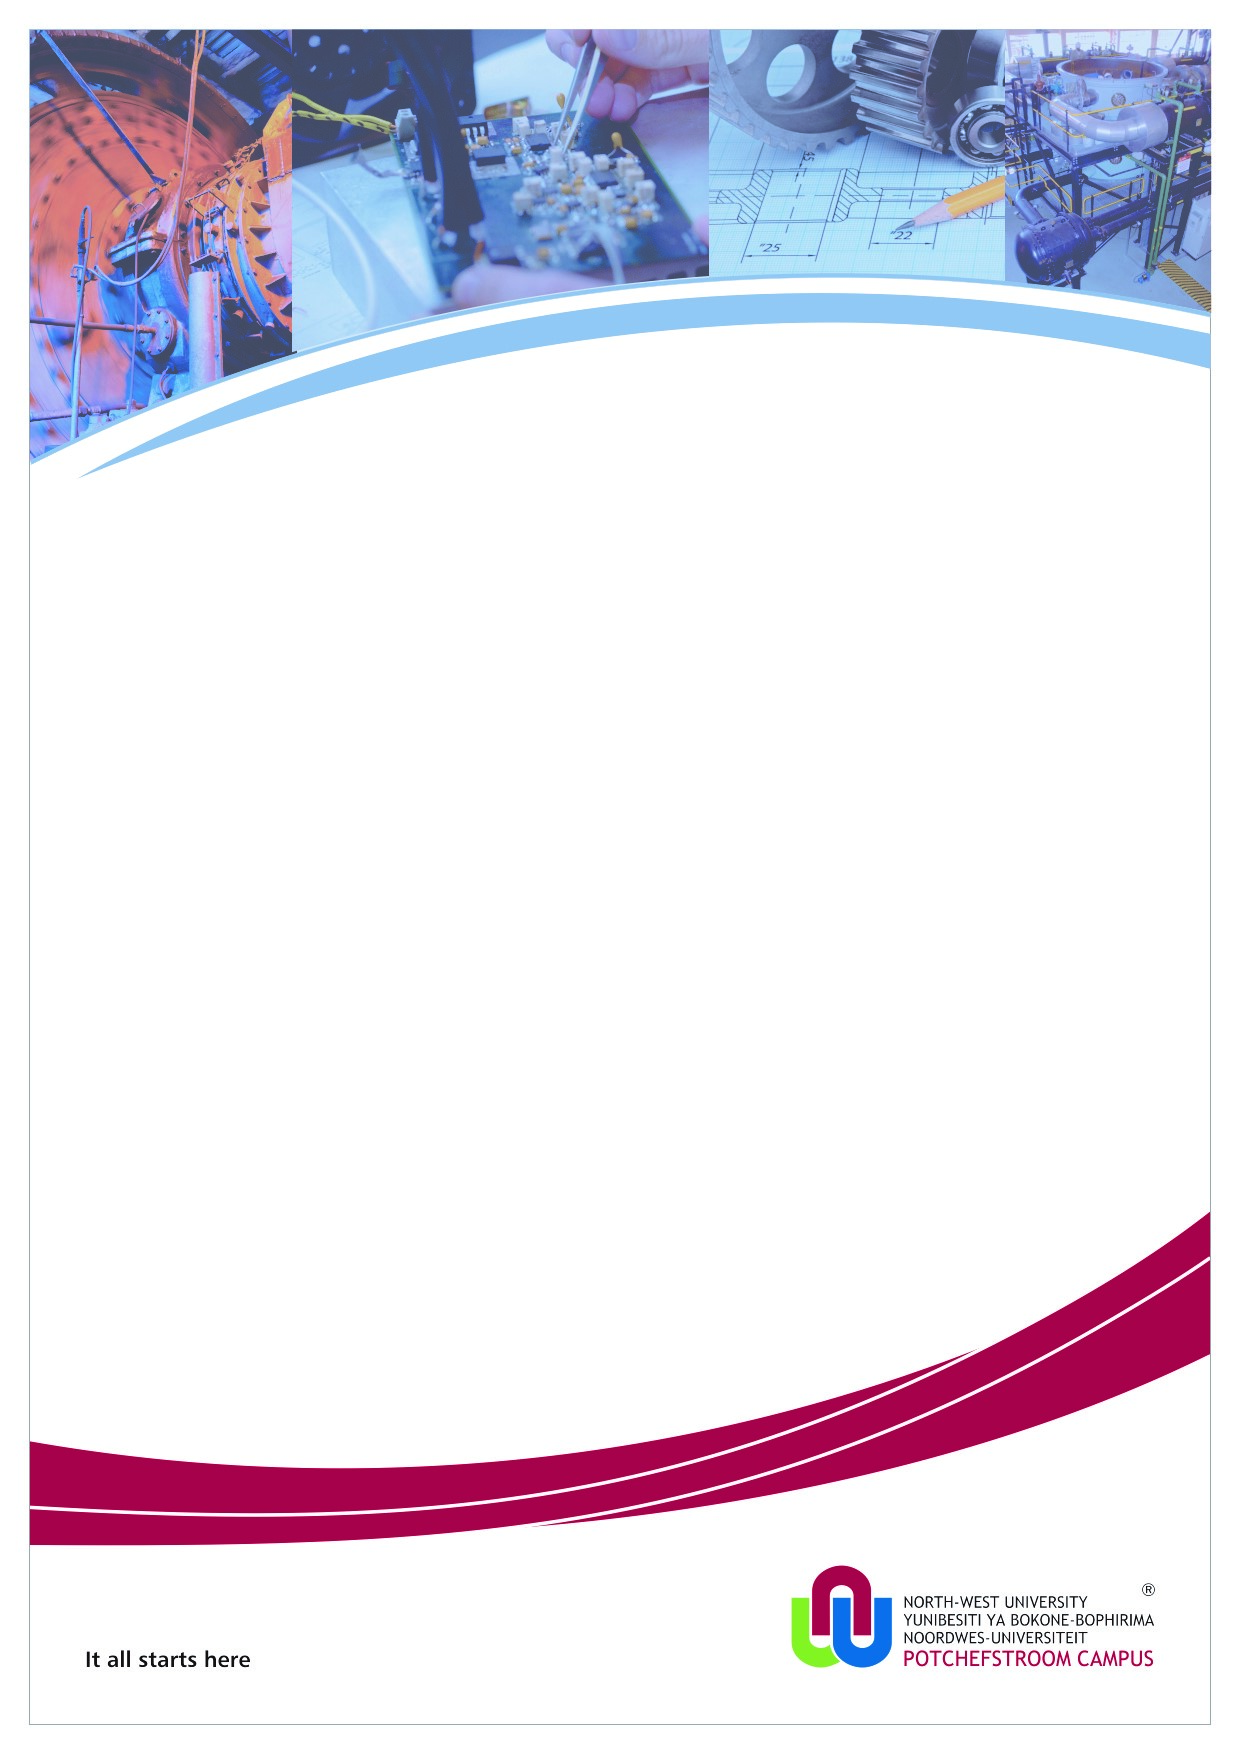
\includegraphics[angle=-45]{frontpage}}





% ****************************************************************************************************
% 8. Further adjustments (experimental)
% ****************************************************************************************************
% ********************************************************************
% Changing the text area
% ********************************************************************
%\linespread{1.05} % a bit more for Palatino
%\areaset[current]{312pt}{761pt} % 686 (factor 2.2) + 33 head + 42 head \the\footskip
%\setlength{\marginparwidth}{7em}%
%\setlength{\marginparsep}{2em}%

% ********************************************************************
% Using different fonts
% ********************************************************************
%\usepackage[oldstylenums]{kpfonts} % oldstyle notextcomp
%\usepackage[osf]{libertine}
%\usepackage{hfoldsty} % Computer Modern with osf
%\usepackage[light,condensed,math]{iwona}
%\renewcommand{\sfdefault}{iwona}
%\usepackage{lmodern} % <-- no osf support :-(
%\usepackage[urw-garamond]{mathdesign} <-- no osf support :-(
% ****************************************************************************************************

\lstset{language=Haskell}
% ****************************************************************************************************  
% If you like the classicthesis, then I would appreciate a postcard. 
% My address can be found in the file ClassicThesis.pdf. A collection 
% of the postcards I received so far is available online at 
% http://postcards.miede.de
% ****************************************************************************************************

% ****************************************************************************************************
% 1. Configure classicthesis for your needs here, e.g., remove "drafting" below 
% in order to deactivate the time-stamp on the pages
% ****************************************************************************************************
\PassOptionsToPackage{eulerchapternumbers,listings,%
				 pdfspacing,%floatperchapter,%linedheaders,%
				 subfig,beramono,eulermath,parts,dottedtoc}{classicthesis}										
% ********************************************************************
% Available options for classicthesis.sty 
% (see ClassicThesis.pdf for more information):
% drafting
% parts nochapters linedheaders
% eulerchapternumbers beramono eulermath pdfspacing minionprospacing
% tocaligned dottedtoc manychapters
% listings floatperchapter subfig
% ********************************************************************

% ********************************************************************
% Triggers for this config
% ******************************************************************** 
\usepackage{ifthen}
\newboolean{enable-backrefs} % enable backrefs in the bibliography
\setboolean{enable-backrefs}{false} % true false
% ****************************************************************************************************


% ****************************************************************************************************
% 2. Personal data and user ad-hoc commands
% ****************************************************************************************************
\newcommand{\myTitle}{Algorithmic Music Composition\xspace}
\newcommand{\mySubtitle}{Composing music algorithmically\xspace}
\newcommand{\myDegree}{B.ENG Computer and Electronic\xspace}
\newcommand{\myName}{Stefan Jacholke\xspace}
\newcommand{\myProf}{Mr. A.J. Alberts\xspace}
\newcommand{\myOtherProf}{Put name here\xspace}
\newcommand{\mySupervisor}{Mr. A.J. Alberts\xspace}
\newcommand{\myFaculty}{Faculty of Engineering\xspace}
\newcommand{\myDepartment}{Put data here\xspace}
\newcommand{\myUni}{North West University - Potchefstroom\xspace}
\newcommand{\myLocation}{Potchefstroom\xspace}
\newcommand{\myTime}{\today\xspace}
\newcommand{\myVersion}{version 2.2\xspace}
\newcommand{\mytilde}{\raise.17ex\hbox{$\scriptstyle\mathtt{\sim}$}}


% ********************************************************************
% Setup, finetuning, and useful commands
% ********************************************************************
\newcounter{dummy} % necessary for correct hyperlinks (to index, bib, etc.)
\newlength{\abcd} % for ab..z string length calculation
\providecommand{\mLyX}{L\kern-.1667em\lower.25em\hbox{Y}\kern-.125emX\@}
\newcommand{\ie}{i.\,e.}
\newcommand{\Ie}{I.\,e.}
\newcommand{\eg}{e.\,g.}
\newcommand{\Eg}{E.\,g.} 
% ****************************************************************************************************


% ****************************************************************************************************
% 3. Loading some handy packages
% ****************************************************************************************************
% ******************************************************************** 
% Packages with options that might require adjustments
% ******************************************************************** 
\PassOptionsToPackage{latin9}{inputenc}	% latin9 (ISO-8859-9) = latin1+"Euro sign"
 \usepackage{inputenc}				

%\PassOptionsToPackage{ngerman,american}{babel}   % change this to your language(s)
% Spanish languages need extra options in order to work with this template
%\PassOptionsToPackage{spanish,es-lcroman}{babel}
 \usepackage{babel}					

\PassOptionsToPackage{square,numbers}{natbib}
 \usepackage{natbib}				

\PassOptionsToPackage{fleqn}{amsmath}		% math environments and more by the AMS 
 \usepackage{amsmath}

% ******************************************************************** 
% General useful packages
% ******************************************************************** 
\PassOptionsToPackage{T1}{fontenc} % T2A for cyrillics
	\usepackage{fontenc}     
\usepackage{textcomp} % fix warning with missing font shapes
\usepackage{scrhack} % fix warnings when using KOMA with listings package          
\usepackage{xspace} % to get the spacing after macros right  
\usepackage{mparhack} % get marginpar right
\usepackage{fixltx2e} % fixes some LaTeX stuff 
\PassOptionsToPackage{printonlyused,smaller}{acronym}
	\usepackage{acronym} % nice macros for handling all acronyms in the thesis
%\renewcommand*{\acsfont}[1]{\textssc{#1}} % for MinionPro
%\renewcommand{\bflabel}[1]{{#1}\hfill} % fix the list of acronyms
% ****************************************************************************************************


% ****************************************************************************************************
% 4. Setup floats: tables, (sub)figures, and captions
% ****************************************************************************************************
\usepackage{tabularx} % better tables
	\setlength{\extrarowheight}{3pt} % increase table row height
\newcommand{\tableheadline}[1]{\multicolumn{1}{c}{\spacedlowsmallcaps{#1}}}
\newcommand{\myfloatalign}{\centering} % to be used with each float for alignment
\usepackage{caption}
\captionsetup{format=hang,font=small}
\usepackage{subfig}  
% ****************************************************************************************************


% ****************************************************************************************************
% 5. Setup code listings
% ****************************************************************************************************
\usepackage{listings} 
%\lstset{emph={trueIndex,root},emphstyle=\color{BlueViolet}}%\underbar} % for special keywords
\lstset{language=[LaTeX]Tex,%C++,
    keywordstyle=\color{RoyalBlue},%\bfseries,
    basicstyle=\small\ttfamily,
    %identifierstyle=\color{NavyBlue},
    commentstyle=\color{Green}\ttfamily,
    stringstyle=\rmfamily,
    numbers=none,%left,%
    numberstyle=\scriptsize,%\tiny
    stepnumber=5,
    numbersep=8pt,
    showstringspaces=false,
    breaklines=true,
    frameround=ftff,
    frame=single,
    belowcaptionskip=.75\baselineskip
    %frame=L
} 
% ****************************************************************************************************    		   


% ****************************************************************************************************
% 6. PDFLaTeX, hyperreferences and citation backreferences
% ****************************************************************************************************
% ********************************************************************
% Using PDFLaTeX
% ********************************************************************
\PassOptionsToPackage{pdftex,hyperfootnotes=false,pdfpagelabels}{hyperref}
	\usepackage{hyperref}  % backref linktocpage pagebackref
\pdfcompresslevel=9
\pdfadjustspacing=1 
\PassOptionsToPackage{pdftex}{graphicx}
	\usepackage{graphicx} 

% ********************************************************************
% Setup the style of the backrefs from the bibliography
% (translate the options to any language you use)
% ********************************************************************
\newcommand{\backrefnotcitedstring}{\relax}%(Not cited.)
\newcommand{\backrefcitedsinglestring}[1]{(Cited on page~#1.)}
\newcommand{\backrefcitedmultistring}[1]{(Cited on pages~#1.)}
\ifthenelse{\boolean{enable-backrefs}}%
{%
		\PassOptionsToPackage{hyperpageref}{backref}
		\usepackage{backref} % to be loaded after hyperref package 
		   \renewcommand{\backreftwosep}{ and~} % separate 2 pages
		   \renewcommand{\backreflastsep}{, and~} % separate last of longer list
		   \renewcommand*{\backref}[1]{}  % disable standard
		   \renewcommand*{\backrefalt}[4]{% detailed backref
		      \ifcase #1 %
		         \backrefnotcitedstring%
		      \or%
		         \backrefcitedsinglestring{#2}%
		      \else%
		         \backrefcitedmultistring{#2}%
		      \fi}%
}{\relax}    

% ********************************************************************
% Hyperreferences
% ********************************************************************
\hypersetup{%
    %draft,	% = no hyperlinking at all (useful in b/w printouts)
    colorlinks=true, linktocpage=true, pdfstartpage=3, pdfstartview=FitV,%
    % uncomment the following line if you want to have black links (e.g., for printing)
    %colorlinks=false, linktocpage=false, pdfborder={0 0 0}, pdfstartpage=3, pdfstartview=FitV,% 
    breaklinks=true, pdfpagemode=UseNone, pageanchor=true, pdfpagemode=UseOutlines,%
    plainpages=false, bookmarksnumbered, bookmarksopen=true, bookmarksopenlevel=1,%
    hypertexnames=true, pdfhighlight=/O,%nesting=true,%frenchlinks,%
    urlcolor=webbrown, linkcolor=RoyalBlue, citecolor=webgreen, %pagecolor=RoyalBlue,%
    %urlcolor=Black, linkcolor=Black, citecolor=Black, %pagecolor=Black,%
    pdftitle={\myTitle},%
    pdfauthor={\textcopyright\ \myName, \myUni, \myFaculty},%
    pdfsubject={},%
    pdfkeywords={},%
    pdfcreator={pdfLaTeX},%
    pdfproducer={LaTeX with hyperref and classicthesis}%
}   

% ********************************************************************
% Setup autoreferences
% ********************************************************************
% There are some issues regarding autorefnames
% http://www.ureader.de/msg/136221647.aspx
% http://www.tex.ac.uk/cgi-bin/texfaq2html?label=latexwords
% you have to redefine the makros for the 
% language you use, e.g., american, ngerman
% (as chosen when loading babel/AtBeginDocument)
% ********************************************************************
\makeatletter
\@ifpackageloaded{babel}%
    {%
       \addto\extrasamerican{%
					\renewcommand*{\figureautorefname}{Figure}%
					\renewcommand*{\tableautorefname}{Table}%
					\renewcommand*{\partautorefname}{Part}%
					\renewcommand*{\chapterautorefname}{Chapter}%
					\renewcommand*{\sectionautorefname}{Section}%
					\renewcommand*{\subsectionautorefname}{Section}%
					\renewcommand*{\subsubsectionautorefname}{Section}% 	
				}%
       \addto\extrasngerman{% 
					\renewcommand*{\paragraphautorefname}{Absatz}%
					\renewcommand*{\subparagraphautorefname}{Unterabsatz}%
					\renewcommand*{\footnoteautorefname}{Fu\"snote}%
					\renewcommand*{\FancyVerbLineautorefname}{Zeile}%
					\renewcommand*{\theoremautorefname}{Theorem}%
					\renewcommand*{\appendixautorefname}{Anhang}%
					\renewcommand*{\equationautorefname}{Gleichung}%        
					\renewcommand*{\itemautorefname}{Punkt}%
				}%	
			% Fix to getting autorefs for subfigures right (thanks to Belinda Vogt for changing the definition)
			\providecommand{\subfigureautorefname}{\figureautorefname}%  			
    }{\relax}
\makeatother


% ****************************************************************************************************
% 7. Last calls before the bar closes
% ****************************************************************************************************
% ********************************************************************
% Development Stuff
% ********************************************************************
\listfiles
%\PassOptionsToPackage{l2tabu,orthodox,abort}{nag}
%	\usepackage{nag}
%\PassOptionsToPackage{warning, all}{onlyamsmath}
%	\usepackage{onlyamsmath}


% Algorithms package
\usepackage[ruled,vlined]{algorithm2e}


\usepackage{booktabs}
%\usepackage[table]{xcolor}


% ****************************************************************************************************
% Rename part name to chapter
% ****************************************************************************************************

\renewcommand\partname{Chapter}


% ********************************************************************
% Last, but not least...
% ********************************************************************
\usepackage{classicthesis} 
% ****************************************************************************************************


% ****************************************************************************************************
% Change ze margins Footer
% ****************************************************************************************************

\usepackage[left=4.0cm,right=4.0cm,top=1.5cm,bottom=2.0cm,includehead,includefoot]{geometry}


% ****************************************************************************************************
% Reduce itemize spacing
% ****************************************************************************************************

\usepackage{enumitem}
\setlist[1]{itemsep=-2pt}


% ****************************************************************************************************
% Ze Footer
% ****************************************************************************************************

  %\renewcommand{\PrelimText}{%
  %\footnotesize\,\today\ -- \texttt{\myTitle}~\myVersion\,}
  %\renewcommand{\finalVersionString}{\emph{Final Version} as of \today\ (\texttt{\@title}~\myVersion).}


% ****************************************************************************************************
% Ze Footer
% ****************************************************************************************************
\usepackage{svg}

\usepackage{pdfpages}


% Front page
\usepackage[firstpage]{draftwatermark}
\usepackage{watermark} 
\SetWatermarkLightness{0.9}
\SetWatermarkText{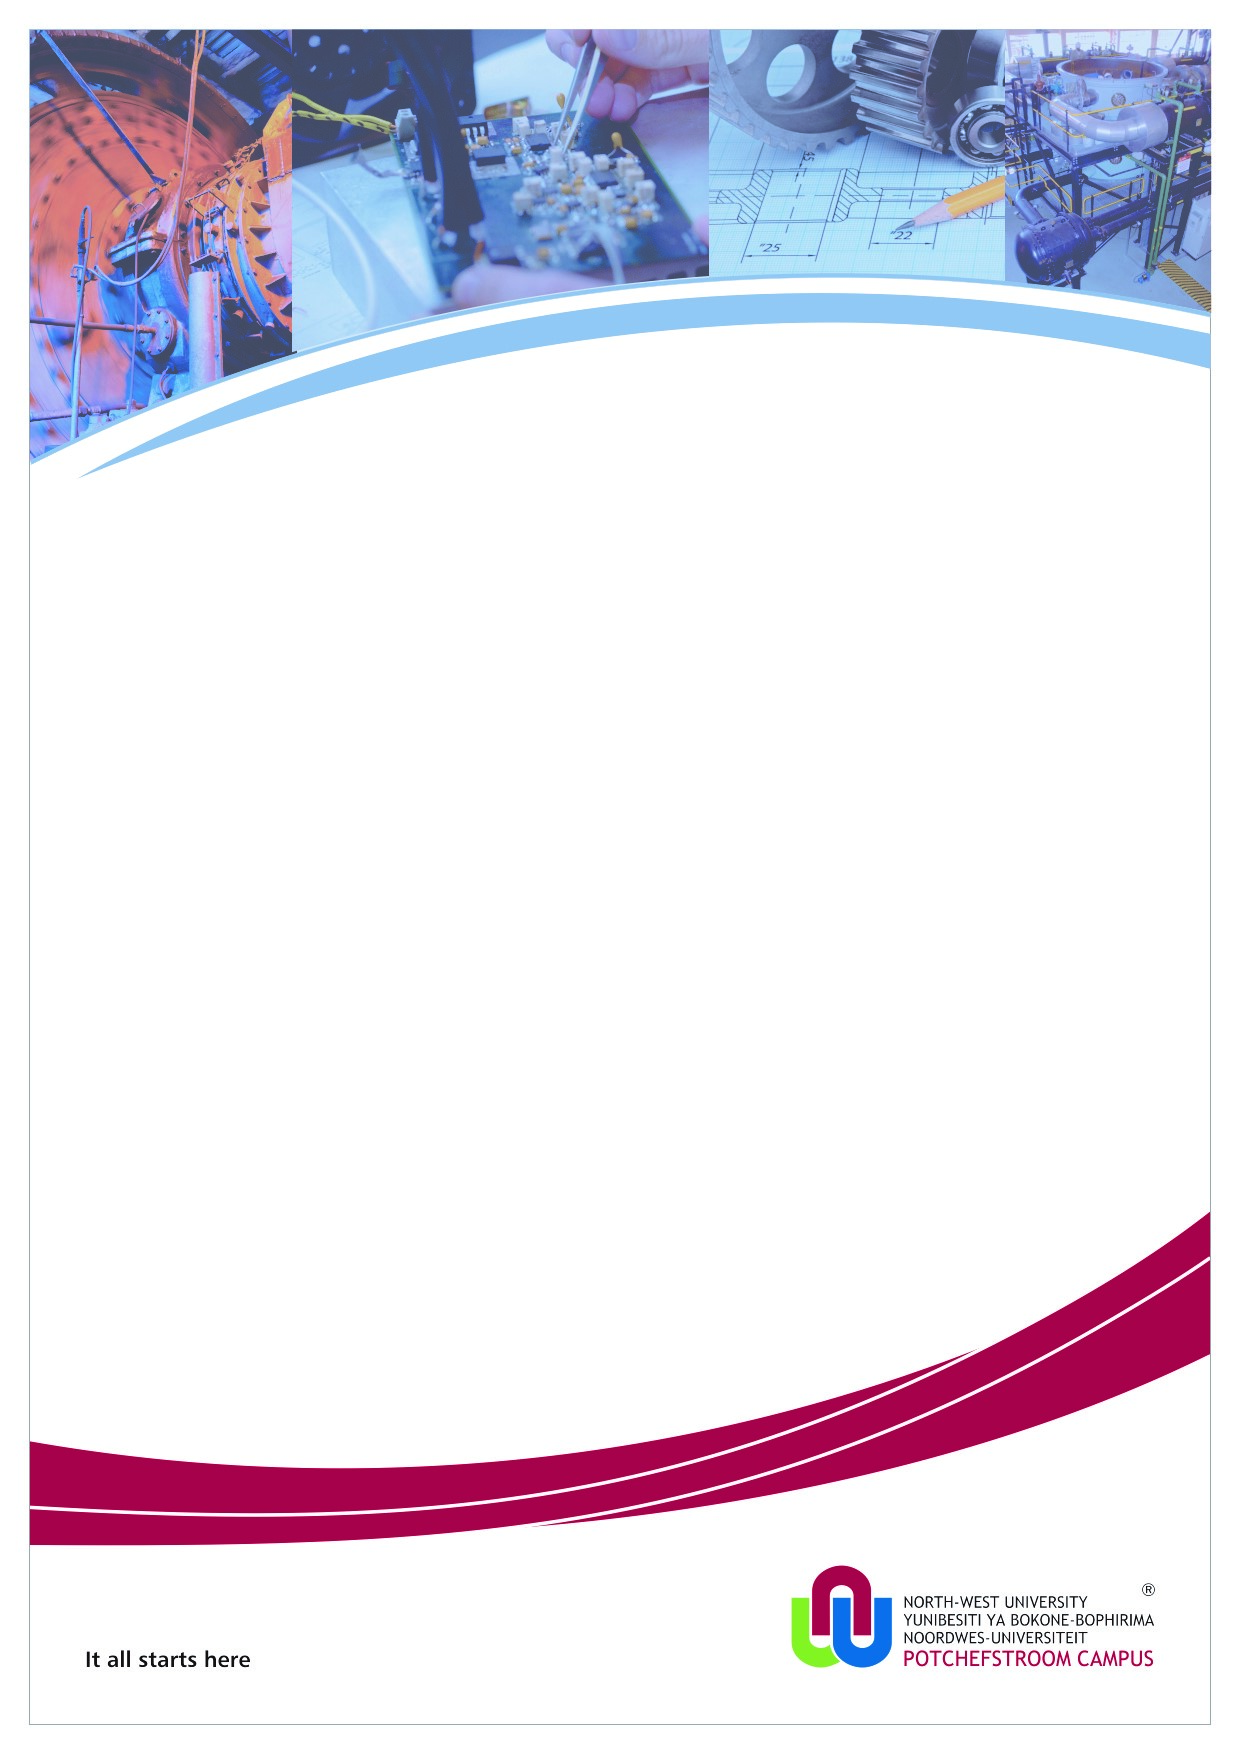
\includegraphics[angle=-45]{frontpage}}





% ****************************************************************************************************
% 8. Further adjustments (experimental)
% ****************************************************************************************************
% ********************************************************************
% Changing the text area
% ********************************************************************
%\linespread{1.05} % a bit more for Palatino
%\areaset[current]{312pt}{761pt} % 686 (factor 2.2) + 33 head + 42 head \the\footskip
%\setlength{\marginparwidth}{7em}%
%\setlength{\marginparsep}{2em}%

% ********************************************************************
% Using different fonts
% ********************************************************************
%\usepackage[oldstylenums]{kpfonts} % oldstyle notextcomp
%\usepackage[osf]{libertine}
%\usepackage{hfoldsty} % Computer Modern with osf
%\usepackage[light,condensed,math]{iwona}
%\renewcommand{\sfdefault}{iwona}
%\usepackage{lmodern} % <-- no osf support :-(
%\usepackage[urw-garamond]{mathdesign} <-- no osf support :-(
% ****************************************************************************************************

\lstset{language=Haskell}
% ****************************************************************************************************  
% If you like the classicthesis, then I would appreciate a postcard. 
% My address can be found in the file ClassicThesis.pdf. A collection 
% of the postcards I received so far is available online at 
% http://postcards.miede.de
% ****************************************************************************************************

% ****************************************************************************************************
% 1. Configure classicthesis for your needs here, e.g., remove "drafting" below 
% in order to deactivate the time-stamp on the pages
% ****************************************************************************************************
\PassOptionsToPackage{eulerchapternumbers,listings,%
				 pdfspacing,%floatperchapter,%linedheaders,%
				 subfig,beramono,eulermath,parts,dottedtoc}{classicthesis}										
% ********************************************************************
% Available options for classicthesis.sty 
% (see ClassicThesis.pdf for more information):
% drafting
% parts nochapters linedheaders
% eulerchapternumbers beramono eulermath pdfspacing minionprospacing
% tocaligned dottedtoc manychapters
% listings floatperchapter subfig
% ********************************************************************

% ********************************************************************
% Triggers for this config
% ******************************************************************** 
\usepackage{ifthen}
\newboolean{enable-backrefs} % enable backrefs in the bibliography
\setboolean{enable-backrefs}{false} % true false
% ****************************************************************************************************


% ****************************************************************************************************
% 2. Personal data and user ad-hoc commands
% ****************************************************************************************************
\newcommand{\myTitle}{Algorithmic Music Composition\xspace}
\newcommand{\mySubtitle}{Composing music algorithmically\xspace}
\newcommand{\myDegree}{B.ENG Computer and Electronic\xspace}
\newcommand{\myName}{Stefan Jacholke\xspace}
\newcommand{\myProf}{Mr. A.J. Alberts\xspace}
\newcommand{\myOtherProf}{Put name here\xspace}
\newcommand{\mySupervisor}{Mr. A.J. Alberts\xspace}
\newcommand{\myFaculty}{Faculty of Engineering\xspace}
\newcommand{\myDepartment}{Put data here\xspace}
\newcommand{\myUni}{North West University - Potchefstroom\xspace}
\newcommand{\myLocation}{Potchefstroom\xspace}
\newcommand{\myTime}{\today\xspace}
\newcommand{\myVersion}{version 2.2\xspace}
\newcommand{\mytilde}{\raise.17ex\hbox{$\scriptstyle\mathtt{\sim}$}}


% ********************************************************************
% Setup, finetuning, and useful commands
% ********************************************************************
\newcounter{dummy} % necessary for correct hyperlinks (to index, bib, etc.)
\newlength{\abcd} % for ab..z string length calculation
\providecommand{\mLyX}{L\kern-.1667em\lower.25em\hbox{Y}\kern-.125emX\@}
\newcommand{\ie}{i.\,e.}
\newcommand{\Ie}{I.\,e.}
\newcommand{\eg}{e.\,g.}
\newcommand{\Eg}{E.\,g.} 
% ****************************************************************************************************


% ****************************************************************************************************
% 3. Loading some handy packages
% ****************************************************************************************************
% ******************************************************************** 
% Packages with options that might require adjustments
% ******************************************************************** 
\PassOptionsToPackage{latin9}{inputenc}	% latin9 (ISO-8859-9) = latin1+"Euro sign"
 \usepackage{inputenc}				

%\PassOptionsToPackage{ngerman,american}{babel}   % change this to your language(s)
% Spanish languages need extra options in order to work with this template
%\PassOptionsToPackage{spanish,es-lcroman}{babel}
 \usepackage{babel}					

\PassOptionsToPackage{square,numbers}{natbib}
 \usepackage{natbib}				

\PassOptionsToPackage{fleqn}{amsmath}		% math environments and more by the AMS 
 \usepackage{amsmath}

% ******************************************************************** 
% General useful packages
% ******************************************************************** 
\PassOptionsToPackage{T1}{fontenc} % T2A for cyrillics
	\usepackage{fontenc}     
\usepackage{textcomp} % fix warning with missing font shapes
\usepackage{scrhack} % fix warnings when using KOMA with listings package          
\usepackage{xspace} % to get the spacing after macros right  
\usepackage{mparhack} % get marginpar right
\usepackage{fixltx2e} % fixes some LaTeX stuff 
\PassOptionsToPackage{printonlyused,smaller}{acronym}
	\usepackage{acronym} % nice macros for handling all acronyms in the thesis
%\renewcommand*{\acsfont}[1]{\textssc{#1}} % for MinionPro
%\renewcommand{\bflabel}[1]{{#1}\hfill} % fix the list of acronyms
% ****************************************************************************************************


% ****************************************************************************************************
% 4. Setup floats: tables, (sub)figures, and captions
% ****************************************************************************************************
\usepackage{tabularx} % better tables
	\setlength{\extrarowheight}{3pt} % increase table row height
\newcommand{\tableheadline}[1]{\multicolumn{1}{c}{\spacedlowsmallcaps{#1}}}
\newcommand{\myfloatalign}{\centering} % to be used with each float for alignment
\usepackage{caption}
\captionsetup{format=hang,font=small}
\usepackage{subfig}  
% ****************************************************************************************************


% ****************************************************************************************************
% 5. Setup code listings
% ****************************************************************************************************
\usepackage{listings} 
%\lstset{emph={trueIndex,root},emphstyle=\color{BlueViolet}}%\underbar} % for special keywords
\lstset{language=[LaTeX]Tex,%C++,
    keywordstyle=\color{RoyalBlue},%\bfseries,
    basicstyle=\small\ttfamily,
    %identifierstyle=\color{NavyBlue},
    commentstyle=\color{Green}\ttfamily,
    stringstyle=\rmfamily,
    numbers=none,%left,%
    numberstyle=\scriptsize,%\tiny
    stepnumber=5,
    numbersep=8pt,
    showstringspaces=false,
    breaklines=true,
    frameround=ftff,
    frame=single,
    belowcaptionskip=.75\baselineskip
    %frame=L
} 
% ****************************************************************************************************    		   


% ****************************************************************************************************
% 6. PDFLaTeX, hyperreferences and citation backreferences
% ****************************************************************************************************
% ********************************************************************
% Using PDFLaTeX
% ********************************************************************
\PassOptionsToPackage{pdftex,hyperfootnotes=false,pdfpagelabels}{hyperref}
	\usepackage{hyperref}  % backref linktocpage pagebackref
\pdfcompresslevel=9
\pdfadjustspacing=1 
\PassOptionsToPackage{pdftex}{graphicx}
	\usepackage{graphicx} 

% ********************************************************************
% Setup the style of the backrefs from the bibliography
% (translate the options to any language you use)
% ********************************************************************
\newcommand{\backrefnotcitedstring}{\relax}%(Not cited.)
\newcommand{\backrefcitedsinglestring}[1]{(Cited on page~#1.)}
\newcommand{\backrefcitedmultistring}[1]{(Cited on pages~#1.)}
\ifthenelse{\boolean{enable-backrefs}}%
{%
		\PassOptionsToPackage{hyperpageref}{backref}
		\usepackage{backref} % to be loaded after hyperref package 
		   \renewcommand{\backreftwosep}{ and~} % separate 2 pages
		   \renewcommand{\backreflastsep}{, and~} % separate last of longer list
		   \renewcommand*{\backref}[1]{}  % disable standard
		   \renewcommand*{\backrefalt}[4]{% detailed backref
		      \ifcase #1 %
		         \backrefnotcitedstring%
		      \or%
		         \backrefcitedsinglestring{#2}%
		      \else%
		         \backrefcitedmultistring{#2}%
		      \fi}%
}{\relax}    

% ********************************************************************
% Hyperreferences
% ********************************************************************
\hypersetup{%
    %draft,	% = no hyperlinking at all (useful in b/w printouts)
    colorlinks=true, linktocpage=true, pdfstartpage=3, pdfstartview=FitV,%
    % uncomment the following line if you want to have black links (e.g., for printing)
    %colorlinks=false, linktocpage=false, pdfborder={0 0 0}, pdfstartpage=3, pdfstartview=FitV,% 
    breaklinks=true, pdfpagemode=UseNone, pageanchor=true, pdfpagemode=UseOutlines,%
    plainpages=false, bookmarksnumbered, bookmarksopen=true, bookmarksopenlevel=1,%
    hypertexnames=true, pdfhighlight=/O,%nesting=true,%frenchlinks,%
    urlcolor=webbrown, linkcolor=RoyalBlue, citecolor=webgreen, %pagecolor=RoyalBlue,%
    %urlcolor=Black, linkcolor=Black, citecolor=Black, %pagecolor=Black,%
    pdftitle={\myTitle},%
    pdfauthor={\textcopyright\ \myName, \myUni, \myFaculty},%
    pdfsubject={},%
    pdfkeywords={},%
    pdfcreator={pdfLaTeX},%
    pdfproducer={LaTeX with hyperref and classicthesis}%
}   

% ********************************************************************
% Setup autoreferences
% ********************************************************************
% There are some issues regarding autorefnames
% http://www.ureader.de/msg/136221647.aspx
% http://www.tex.ac.uk/cgi-bin/texfaq2html?label=latexwords
% you have to redefine the makros for the 
% language you use, e.g., american, ngerman
% (as chosen when loading babel/AtBeginDocument)
% ********************************************************************
\makeatletter
\@ifpackageloaded{babel}%
    {%
       \addto\extrasamerican{%
					\renewcommand*{\figureautorefname}{Figure}%
					\renewcommand*{\tableautorefname}{Table}%
					\renewcommand*{\partautorefname}{Part}%
					\renewcommand*{\chapterautorefname}{Chapter}%
					\renewcommand*{\sectionautorefname}{Section}%
					\renewcommand*{\subsectionautorefname}{Section}%
					\renewcommand*{\subsubsectionautorefname}{Section}% 	
				}%
       \addto\extrasngerman{% 
					\renewcommand*{\paragraphautorefname}{Absatz}%
					\renewcommand*{\subparagraphautorefname}{Unterabsatz}%
					\renewcommand*{\footnoteautorefname}{Fu\"snote}%
					\renewcommand*{\FancyVerbLineautorefname}{Zeile}%
					\renewcommand*{\theoremautorefname}{Theorem}%
					\renewcommand*{\appendixautorefname}{Anhang}%
					\renewcommand*{\equationautorefname}{Gleichung}%        
					\renewcommand*{\itemautorefname}{Punkt}%
				}%	
			% Fix to getting autorefs for subfigures right (thanks to Belinda Vogt for changing the definition)
			\providecommand{\subfigureautorefname}{\figureautorefname}%  			
    }{\relax}
\makeatother


% ****************************************************************************************************
% 7. Last calls before the bar closes
% ****************************************************************************************************
% ********************************************************************
% Development Stuff
% ********************************************************************
\listfiles
%\PassOptionsToPackage{l2tabu,orthodox,abort}{nag}
%	\usepackage{nag}
%\PassOptionsToPackage{warning, all}{onlyamsmath}
%	\usepackage{onlyamsmath}


% Algorithms package
\usepackage[ruled,vlined]{algorithm2e}


\usepackage{booktabs}
%\usepackage[table]{xcolor}


% ****************************************************************************************************
% Rename part name to chapter
% ****************************************************************************************************

\renewcommand\partname{Chapter}


% ********************************************************************
% Last, but not least...
% ********************************************************************
\usepackage{classicthesis} 
% ****************************************************************************************************


% ****************************************************************************************************
% Change ze margins Footer
% ****************************************************************************************************

\usepackage[left=4.0cm,right=4.0cm,top=1.5cm,bottom=2.0cm,includehead,includefoot]{geometry}


% ****************************************************************************************************
% Reduce itemize spacing
% ****************************************************************************************************

\usepackage{enumitem}
\setlist[1]{itemsep=-2pt}


% ****************************************************************************************************
% Ze Footer
% ****************************************************************************************************

  %\renewcommand{\PrelimText}{%
  %\footnotesize\,\today\ -- \texttt{\myTitle}~\myVersion\,}
  %\renewcommand{\finalVersionString}{\emph{Final Version} as of \today\ (\texttt{\@title}~\myVersion).}


% ****************************************************************************************************
% Ze Footer
% ****************************************************************************************************
\usepackage{svg}

\usepackage{pdfpages}


% Front page
\usepackage[firstpage]{draftwatermark}
\usepackage{watermark} 
\SetWatermarkLightness{0.9}
\SetWatermarkText{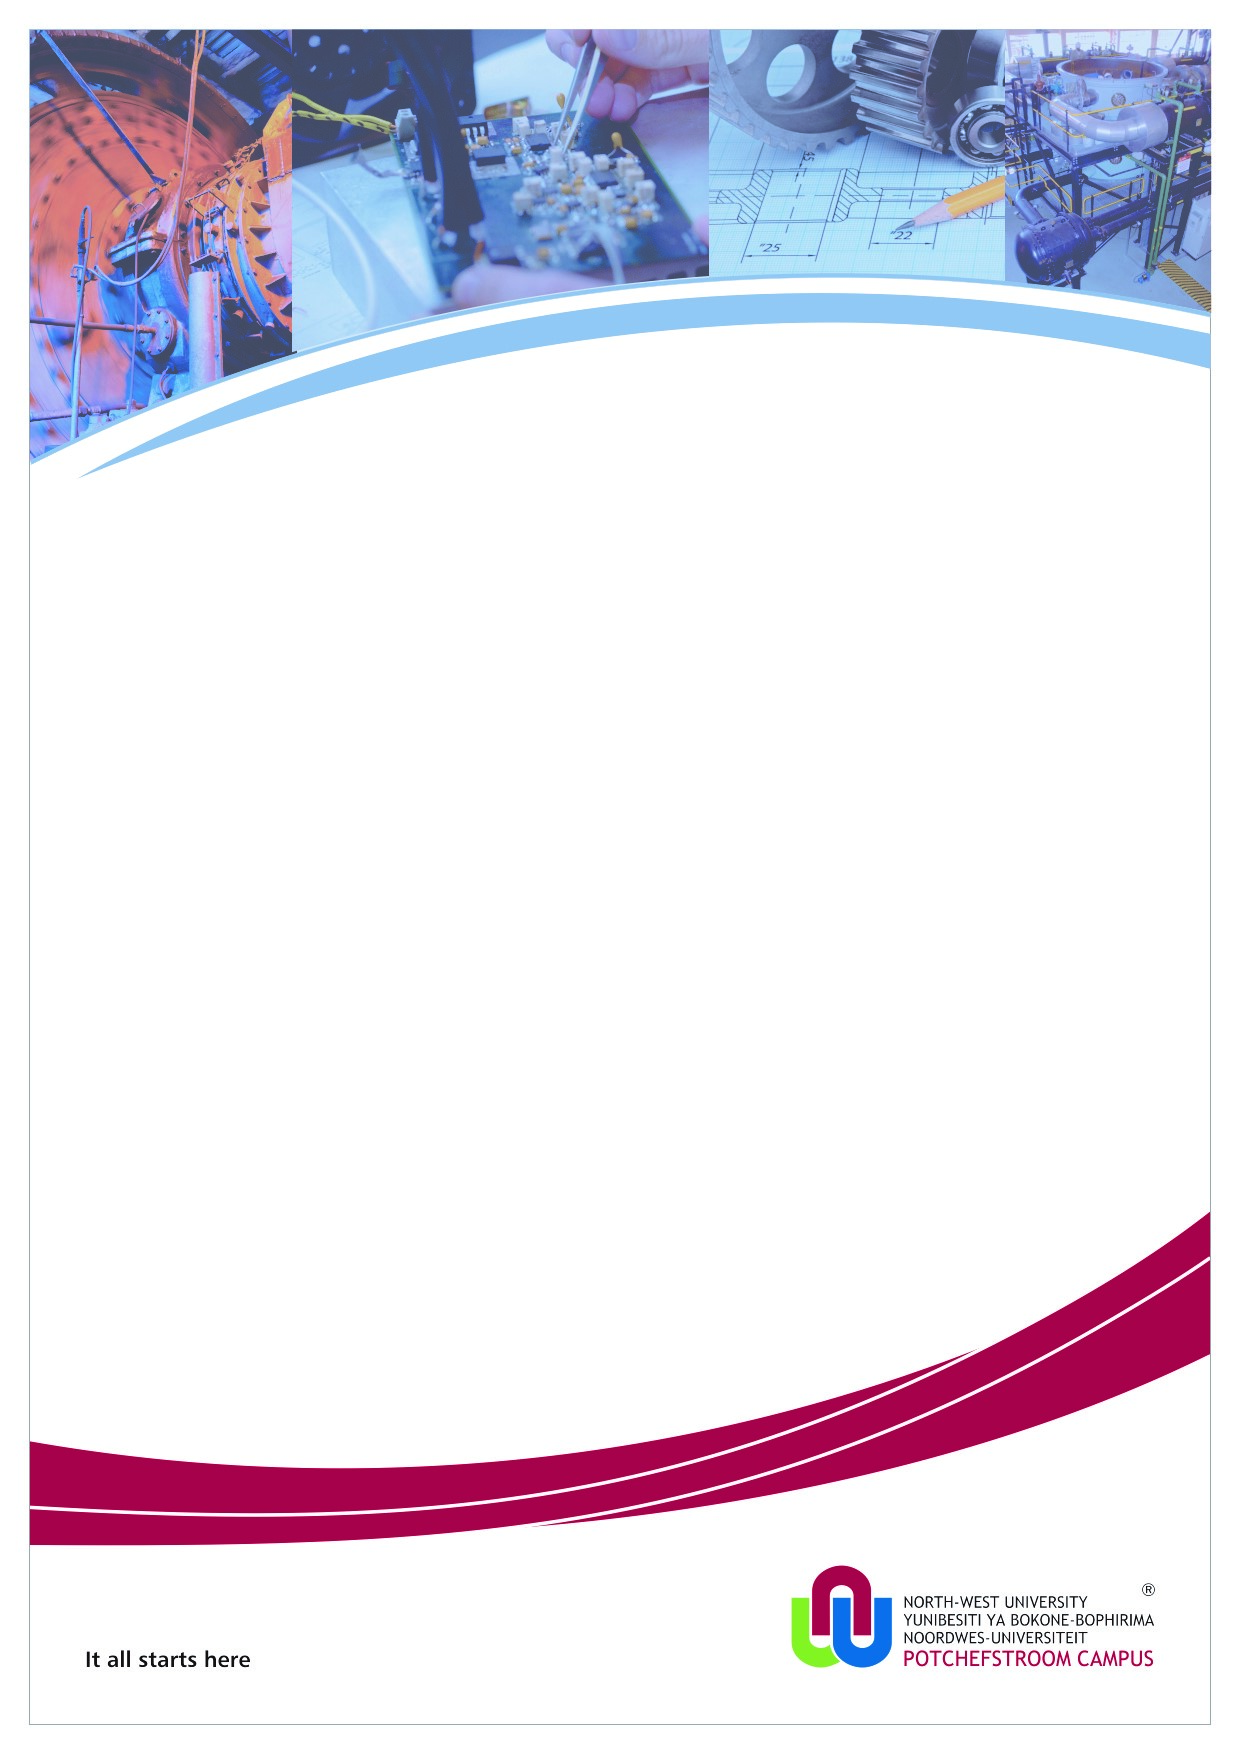
\includegraphics[angle=-45]{frontpage}}





% ****************************************************************************************************
% 8. Further adjustments (experimental)
% ****************************************************************************************************
% ********************************************************************
% Changing the text area
% ********************************************************************
%\linespread{1.05} % a bit more for Palatino
%\areaset[current]{312pt}{761pt} % 686 (factor 2.2) + 33 head + 42 head \the\footskip
%\setlength{\marginparwidth}{7em}%
%\setlength{\marginparsep}{2em}%

% ********************************************************************
% Using different fonts
% ********************************************************************
%\usepackage[oldstylenums]{kpfonts} % oldstyle notextcomp
%\usepackage[osf]{libertine}
%\usepackage{hfoldsty} % Computer Modern with osf
%\usepackage[light,condensed,math]{iwona}
%\renewcommand{\sfdefault}{iwona}
%\usepackage{lmodern} % <-- no osf support :-(
%\usepackage[urw-garamond]{mathdesign} <-- no osf support :-(
% ****************************************************************************************************

\lstset{language=Haskell}

%********************************************************************
% Hyphenation
%*******************************************************
%\hyphenation{put special hyphenation here}

% ********************************************************************
% GO!GO!GO! MOVE IT!
%*******************************************************
\begin{document}
\frenchspacing
\raggedbottom
\selectlanguage{american} % american ngerman
%\renewcommand*{\bibname}{new name}
%\setbibpreamble{}
\pagenumbering{roman}
\pagestyle{plain}
%********************************************************************
% Frontmatter
%*******************************************************
%!TEX root = ../Report.tex
%*******************************************************
% Little Dirty Titlepage
%*******************************************************


\thispagestyle{empty}
\begin{titlepage}
\thispagestyle{empty}


%\begin{addmargin}[-1cm]{-3cm}
\begin{center}
\large

\hfill
\vfill
\vfill
\begingroup
\color{Maroon}\Large{\spacedallcaps{Algorithmic music composition}} \\ \bigskip % Thesis title
\endgroup
\vspace{5mm}
by: \\
 \begin{tabular}{l  r} 
 S. Jacholke & 23671750 \\

 \end{tabular}			\\
 
\vfill

submitted in persuit of the degree\\
\vspace{8mm}

\spacedallcaps{Bachelor of engineering}\\

in\\

\spacedallcaps{computer and electronic engineering}\\

\vfill

\textbf{North-West University  Potchefstroom Campus}\\

			
\vspace*{0.8cm}

\begin{flushleft}
Supervisor: \mySupervisor

\myLocation

\myTime

\myVersion

\end{flushleft}



\vfill

\end{center}
%\end{addmargin}

\end{titlepage}






%%*******************************************************
% Titlepage
%*******************************************************


\begin{titlepage}
	% if you want the titlepage to be centered, uncomment and fine-tune the line below (KOMA classes environment)
	\begin{addmargin}[-1cm]{-3cm}
    \begin{center}
        \large  

        \hfill

        \vfill

        \begingroup
            \color{Maroon}\spacedallcaps{\myTitle} \\ \bigskip
        \endgroup

        \spacedlowsmallcaps{\myName}

        \vfill

        \includegraphics[width=14cm]{gfx/comp_logo} \\ \medskip

        \mySubtitle \\ \medskip   
        %\myDegree \\
        %\myDepartment \\                            
        %\myFaculty \\
        %\myUni \\ \bigskip

        \myTime\ -- \myVersion

        \vfill                      

    \end{center}  
  \end{addmargin}       
\end{titlepage}   
\thispagestyle{empty}

\hfill

\vfill

\noindent\myName: \textit{\myTitle,} \mySubtitle, %\myDegree, 
\textcopyright\ \myTime

%\bigskip
%
%\noindent\spacedlowsmallcaps{Supervisors}: \\
%\myProf \\
%\myOtherProf \\ 
%\mySupervisor
%
%\medskip
%
%\noindent\spacedlowsmallcaps{Location}: \\
%\myLocation
%
%\medskip
%
%\noindent\spacedlowsmallcaps{Time Frame}: \\
%\myTime

%\cleardoublepage%*******************************************************
% Dedication
%*******************************************************
\thispagestyle{empty}
%\phantomsection 
\refstepcounter{dummy}
\pdfbookmark[1]{Dedication}{Dedication}

\vspace*{3cm}

\begin{center}
    \emph{Ohana} means family. \\
    Family means nobody gets left behind, or forgotten. \\ \medskip
    --- Lilo \& Stitch    
\end{center}

\medskip

\begin{center}
    Dedicated to the loving memory of Rudolf Miede. \\ \smallskip
    1939\,--\,2005
\end{center}
%\cleardoublepage\include{FrontBackmatter/Foreword}
\cleardoublepage%!TEX root = ../Report.tex
%*******************************************************
% Declaration
%*******************************************************
%\refstepcounter{dummy}
%\pdfbookmark[0]{Declaration}{declaration}
\chapter*{Declaration}
\thispagestyle{empty}
I, Stefan Jacholke hereby declare that the report and all work associated with the `Algorithmic Music Composition' project is my own original work and had not already been submitted to any university or institution for examination
\bigskip
 
\noindent\textit{\myLocation, \myTime}

\smallskip

\begin{flushright}
    \begin{tabular}{m{5cm}}
    
\includegraphics[width=100px]{../images/sjacholke_signature.png}
        \\ \hline
        \centering\myName \\
    \end{tabular}
\end{flushright}

\cleardoublepage%!TEX root = ../Report.tex
%*******************************************************
% Abstract
%*******************************************************
%\renewcommand{\abstractname}{Abstract}
\pdfbookmark[1]{Abstract}{Abstract}
\begingroup
\let\clearpage\relax
\let\cleardoublepage\relax
\let\cleardoublepage\relax




\chapter*{Abstract}




The field of algorithmic music composition is not new. The problem of algorithmically composing music is difficult and there is a wide range of research on the topic however, this field is inaccessible to most.
\\
\\
This project covered a survey on algorithmic music composition and what it entails. In order to generate music in a certain style that is specified by the user, machine learning algorithms were used with the input dataset being one that corresponds to a certain style.
\\
\\
Various algorithms were investigated, designed and implemented. The best few were kept for inclusion in the developed friendly end-user application which exposes algorithmic music composition with machine learning to those who are not literate in the field. The application allows the user to select a musical category and generate a monophonic melody using certain algorithms. The result can be visually displayed, played and stored.
\\
\\
Since it is difficult to quantify the pleasantness of a song, due to the inherent subjective experience, it was necessary to rely on statistical features and probabilistic models. The algorithms investigated include Hidden Markov Models, Markov Chains, Neural Networks, Stochastic Sampling and Genetic Algorithms. These algorithms are discussed and compared.
\\
\\
The weakness of the algorithms implemented is that they do not have an overarching theme or structure. 



\vfill

%\pdfbookmark[1]{Zusammenfassung}{Zusammenfassung}
%\chapter*{Zusammenfassung}
%Kurze Zusammenfassung des Inhaltes in deutscher Sprache\dots


\endgroup			

\vfill
%\cleardoublepage%*******************************************************
% Publications
%*******************************************************
\pdfbookmark[1]{Publications}{publications}
\chapter*{Publications}
Some ideas and figures have appeared previously in the following publications:

\bigskip

\noindent Put your publications from the thesis here. The packages \texttt{multibib} or \texttt{bibtopic} etc. can be used to handle multiple different bibliographies in your document.
%\cleardoublepage%*******************************************************
% Acknowledgments
%*******************************************************
\pdfbookmark[1]{Acknowledgments}{acknowledgments}

\begin{flushright}{\slshape    
    We have seen that computer programming is an art, \\ 
    because it applies accumulated knowledge to the world, \\ 
    because it requires skill and ingenuity, and especially \\
    because it produces objects of beauty.} \\ \medskip
    --- \defcitealias{knuth:1974}{Donald E. Knuth}\citetalias{knuth:1974} \citep{knuth:1974}
\end{flushright}



\bigskip

\begingroup
\let\clearpage\relax
\let\cleardoublepage\relax
\let\cleardoublepage\relax
\chapter*{Acknowledgments}
Put your acknowledgments here.

Many thanks to everybody who already sent me a postcard!

Regarding the typography and other help, many thanks go to Marco 
Kuhlmann, Philipp Lehman, Lothar Schlesier, Jim Young, Lorenzo 
Pantieri and Enrico Gregorio\footnote{Members of GuIT (Gruppo 
Italiano Utilizzatori di \TeX\ e \LaTeX )}, J\"org Sommer, 
Joachim K\"ostler, Daniel Gottschlag, Denis Aydin, Paride 
Legovini, Steffen Prochnow, Nicolas Repp, Hinrich Harms, 
 Roland Winkler, J\"org Weber, 
 and the whole \LaTeX-community for support, ideas and 
 some great software.

\bigskip

\noindent\emph{Regarding \mLyX}: The \mLyX\ port was intially done by 
\emph{Nicholas Mariette} in March 2009 and continued by 
\emph{Ivo Pletikosi\'c} in 2011. Thank you very much for your 
work and the contributions to the original style.


\endgroup




\pagestyle{scrheadings}
\cleardoublepage%!TEX root = ../Report.tex
%*******************************************************
% Table of Contents
%*******************************************************
%\phantomsection
\refstepcounter{dummy}
\pdfbookmark[1]{\contentsname}{tableofcontents}
\setcounter{tocdepth}{2} % <-- 2 includes up to subsections in the ToC
\setcounter{secnumdepth}{3} % <-- 3 numbers up to subsubsections
\manualmark
\markboth{\spacedlowsmallcaps{\contentsname}}{\spacedlowsmallcaps{\contentsname}}
\tableofcontents 
\automark[section]{chapter}
\renewcommand{\chaptermark}[1]{\markboth{\spacedlowsmallcaps{#1}}{\spacedlowsmallcaps{#1}}}
\renewcommand{\sectionmark}[1]{\markright{\thesection\enspace\spacedlowsmallcaps{#1}}}
%*******************************************************
% List of Figures and of the Tables
%*******************************************************
\clearpage

\begingroup 
    \let\clearpage\relax
    \let\cleardoublepage\relax
    \let\cleardoublepage\relax
    %*******************************************************
    % List of Figures
    %*******************************************************    
    %\phantomsection 
    \refstepcounter{dummy}
    %\addcontentsline{toc}{chapter}{\listfigurename}
    \pdfbookmark[1]{\listfigurename}{lof}
    \listoffigures

    \vspace*{8ex}

    %*******************************************************
    % List of Tables
    %*******************************************************
    %\phantomsection 
    \refstepcounter{dummy}
    %\addcontentsline{toc}{chapter}{\listtablename}
    \pdfbookmark[1]{\listtablename}{lot}
    \listoftables
        
    \vspace*{8ex}
%   \newpage
    
    %*******************************************************
    % List of Listings
    %*******************************************************      
	  %\phantomsection 
    \refstepcounter{dummy}
    %\addcontentsline{toc}{chapter}{\lstlistlistingname}
    \pdfbookmark[1]{\lstlistlistingname}{lol}
    \lstlistoflistings 

    \vspace*{8ex}
       
    %*******************************************************
    % Acronyms
    %*******************************************************
    %\phantomsection 
    \refstepcounter{dummy}
    \pdfbookmark[1]{Acronyms}{acronyms}
    \markboth{\spacedlowsmallcaps{Acronyms}}{\spacedlowsmallcaps{Acronyms}}
    \pagebreak
    \chapter*{Acronyms}
    \begin{acronym}[UML]
        \acro{ANN}{Artificial Neural Network}
        \acro{GP}{Genetic Program}
        \acro{GA}{Genetic Algorithm}
        \acro{HMM}{Hidden Markov Model}
        \acro{GMM}{Gaussian Mixture Model }
        \acro{MIDI}{Musical Instrument Digital Interface}
        \acro{NCD}{Normalized Compression Distance}
        \acro{NID}{Normalized Information Distance}
        \acro{IGA}{Interactive Genetic Algorithm}
        \acro{SRN}{Simple Recurrent Network}
        \acro{LTSM}{Long term short term}
        \acro{ART}{Adapative resonance theory}
        \acro{RNN}{Recurrent neural network}

    \end{acronym}     
       

\endgroup

\cleardoublepage
%********************************************************************
% Mainmatter
%*******************************************************
\pagenumbering{arabic}
%\setcounter{page}{90}
% use \cleardoublepage here to avoid problems with pdfbookmark
\cleardoublepage
\part{Introduction}
%!TEX root = ../Report.tex
\chapter{Algorithmic Music Composition}
\section{Introduction}
Music is the art form of sound. Certain characteristics and patterns can be identified that belong to certain types of music.


There has been a lot of work done in computer generated music and computer assisted music composition.The design of computational methods for musical style imitation has been far more difficult than initially imagined.
Recent research into music composition by means of evolutionary genetic algorithms and other machine learning algorithms such as neural networks have met some success.

Music generated algorithmically by computers might some day share the success known by modern and historic music. In a hypothetical time period artists might compete with algorithmic composers.

Computer generated music is an old idea, however existing solutions that generate music use outdated procedural algorithms and do not match the quality of proper historic music. The variety and quality of existing solutions is limited. Most current solutions were implemented to accommodate the research being done and are not suitable for end-users.

This section will outline the problems that are encountered with conventional music composition and a solution is proposed. Some of the ideas behind systems that learn music composition will be outlined and described. The problem of implementing and creating a solution will be detailed as well as the steps required to complete such a project.

\section{Problem}
In order to avoid copyright infringement music has to be licensed for use in commercial applications. Small business owners, independent developers and other smaller organizations may not have the required funding in order to obtain the relevant licensing.

The alternative solution is to produce the required music self, however this requires time and skill.

A solution to this problem is to generate music by artificial intelligent means. 
Algorithmic music composition is of theoretical interest and research has been done for composing music by genetic algorithms and neural networks, amongst other algorithms.

A software application that is able to compose and play monophonic melodies according to a certain style by means of machine learning algorithms could solve the licensing and resource problem.

\section{Solution}
\begin{figure}
\centerline{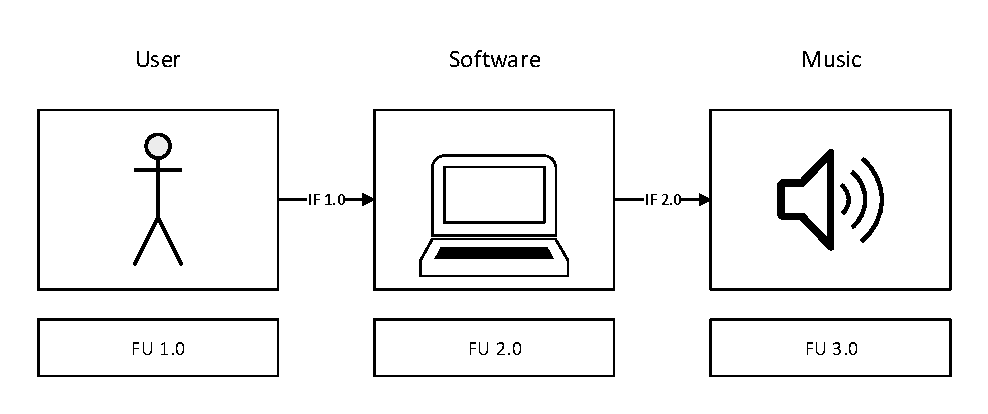
\includegraphics[width=300px]{../images/arch.pdf}}
\caption{Figure of high-level architecture of project}
\label{ims:archm}
\end{figure}

The solution to the problem is to create an application that is capable of composing and playing simple monophonic melodies using machine learning algorithms. Algorithms other than learning algorithms may be used, however these algorithms are narrow in application. Using learning algorithms and pattern recognition allows the application to produce melodies according to a selected style.

There is a need for a user-friendly application that can be used to generate simple monophonic melodies according to a certain style or category of music.
The application is required to have the following features :
\begin{enumerate}
\item Melodies are to be algorithmically composed according to a certain style.
\item Provide playback functionality as well as saving and loading of previously composed songs.
\item The user should be able to select the style
\item The application should utilize a \acs{MIDI} library which will be used as training data for the machine learning algorithms.
\end{enumerate}

Figure \ref{ims:archm} indicates the interaction between the user and the software.

Since the quality and aesthetics of a musical melody is subjective, it is beyond the scope of the application to ensure that each melody produced is objectively good\footnote{The focus is rather on the generated musical pieces not being objectively bad}. Composed musical pieces will take the form of simple melodies.

\section{Alternative solutions}
A wide variety of research has been done and in this section we will briefly look at some of the existing solutions and their drawbacks

\subsubsection{NEUROGEN}
NEUROGEN is a system that was designed to compose small diatonic, western-type, four part harmony compositions based on a training set of example musical fragments. NEUROGEN tries to produce coherent music of the type that is typically found in traditionally hymns \cite{gibson1991neurogen}.
However NEUROGEN is only tries to fulfill its main research goals.

\subsubsection{CONCERT}
CONCERT incorporates psychologically-grounded representations of pitch, duration and harmonic structure in order to compose novel melodies. CONCERT uses a neural network in order to do note by note predictions. 

CONCERT struggles to compose natural music as the music produced was not globally coherent \cite{mozer1994neural}. 

CONCERT also only tries to fulfill its research goals, that is, to compose music on a note by note basis using a neural network.

More recent studies into recurrent neural networks based on \ac{LSTM} indicate that it is indeed possible to compose music using recurrent neural networks that have global structure \cite{Eck2002}.

\subsubsection{GenJam}
GenJam - Genetic Jammer is a \acs{IGA} that learns to improvise jazz \cite{Biles1994}.
The system is able to: 
\begin{enumerate}
\item Play full-chorus improvised solos
\item Respond interactively when the trumpet is played to trade fours or eights
\item Perform a smart echo of improvisation
\end{enumerate}

The main drawback of GenJam is that it is an interactive algorithm and as such requires input from the user. The creates a performance bottleneck as it is time consuming for the user to rate musical pieces.
See section \ref{sec:iga} for work on \acsp{IGA}

\subsection{jMusic}
jMusic is an application and library that facilitates musical composition in Java \cite{Sorensen}. The application is designed to provide composers and developers a plethora of compositional tools that can be used for generative music, instrument building, interactive performance and music analysis. In addition the software provides the following:
\begin{itemize}
\item Familar music data structures
\item Organizing, manipulating and analyzing music data
\item Real time playback of music scores
\item Read, write \ac{MIDI}, \ac{XML} and .jm files
\end{itemize}

jMusic is mostly a developer tool to facilitate composition. It does not feature a user interface which can be used to easily generate compositions. Furthermore since it is mostly a tool to aid music composition it does not employ machine learning algorithms. The library requires exact and descriptive input in order to generate melodies, and as such requires domain knowledge.

\subsubsection{Other}
Most of the work done in the field has been aimed on narrow application of the ideas being investigated. Thus algorithms and applications constructed were aimed only to experimentally study the ideas being investigated and not to serve as a end-user product. 

Some other small application exist which employ \acp{IGA} such as:
\begin{enumerate}
\item \href{http://askory.phratry.net/projects/evolutune/}{Evolutune}\footnote{http://askory.phratry.net/projects/evolutune/}
\item \href{http://www.compose-music.com/}{Song Builder}\footnote{http://www.compose-music.com/}
\item \href{http://game.darwintunes.org/}{DarwinTunes}\footnote{http://game.darwintunes.org/}
\end{enumerate}

Even though more recent research into algorithmic music composition yields promising results there is no single application combining the more recent research into a coherent application that is able to play monophonic melodies\footnote{In addition there is no accessible user-friendly application that expose machine learning based algorithmic composition to the user}.


\section{Feasibility}
There has been a plethora of research done into algorithmic music composition. Some of the more recent research that utilizes machine learning algorithms is investigated in chapter \ref{chap:comp_algo}.

Some machine learning methods to compose music algorithmically include:
\begin{itemize}
\item Recurrent neural networks \cite{Eck2002, mozer1994neural,Chen2001}
\item Genetic algorithms using \acs{NCD} as fitness functions \cite{Alfonseca2006,Dostal2013}
\item Genetic algorithms using neural networks as fitness functions \cite{gibson1991neurogen,Biles1996,Burton97geneticalgorithm}
\item Genetic algorithms employing Zipf's law and cosine similarity \cite{Dostal2013,Manaris2007,Manaris2005}
\item Interactive genetic algorithms \cite{Biles1994, Biles1996,Unehara,Spector_inductionand,Johanson1998}
\item Markov Chains for music composition \cite{McAlpine1999, Farbood2001}.
\item Hidden Markov Models for harmonization \cite{Allan2004}.
\item LSTM neural network for composing blues \cite{Eck2002}.
\end{itemize}

A variety of ideas and techniques in algorithmic music composition have already been researched. The difficulty arises in the implementation of the ideas (as the process is only fundamentally documented), representation of music in data structures and the implementation of the relevant machine learning algorithms.

\section{Methodology}
In Royce's classical waterfall model the following steps are followed when developing software:
\begin{itemize}
\item Requirements specification
\item Design resulting in the software architecture
\item Construction
\item Integration
\item Testing and debugging
\item Installation
\item Maintenance
\end{itemize}

Since there are a variety of algorithmic music composition strategies, and no formal analysis that compares the quality of the resulting music of each strategy (difficult as it is a subjective matter) the software prototyping methodology could be used to test these different ideas and to construct a trade-off study to determine the most feasible techniques.
\\
\\
Software prototyping is the development of prototypes - incomplete versions of the software.
Some basic principles of software prototyping include:
\begin{itemize}
\item Prototype selected parts
\item Breaking project into smaller segments
\item User or client may be involved
\item Iterative modification to meet user demands
\end{itemize}

The main ideas of the systems engineering process, as applicable to software will be followed. Ideas from the waterfall model and software prototyping will be incorporated.

The basic formulation of the design of the project is as follows:
\begin{enumerate}
\item Conceptual design
\begin{itemize}
\item Identify problem
\item Identify requirements
\item Resource allocation
\item Literature study
\item Feasibility analysis
\item Trade off study
\end{itemize}
\item Preliminary design
\item Detail design
\begin{itemize}
\item Design of software architecture
\item Prototyping of different strategies and algorithms
\end{itemize}
\item Construction
\begin{itemize}
\item Code is written
\item Code is tested
\item Iteratively improve until project meets specifications
\end{itemize}
\item Phase out, support, maintenance
\end{enumerate}

In order to identify suitable algorithms a literature review will be done. The various algorithms will be prototyped and tested and the best few resulting algorithms will be used. Software development will follow the waterfall model.

\pagebreak
\section{Conclusion}
Since the act of generating music using algorithmic means is of theoretical interest there is a plethora of research available, however most of these implementations only aim to explore the main idea being researched. Thus there is a lack of accessible, user-friendly applications that are able to generate music algorithmically.

The aim of this project is to construct an application that is able to compose music algorithmically. The application will utilize machine learning algorithms in order to compose monophonic melodies according to the style of a certain author or theme. These ideas have already been researched and thus the application is feasible. The only cost is time and effort.

The methodology for successfully completing the project is outlined and a schedule for completing each goal is presented. This should assist in meeting the deadlines and completing the project successfully according to the specifications. 
\part{Literature Review}
%!TEX root = ../Report.tex
%************************************************
\chapter{Music and music-representation}\label{ch:introduction}
\section{Musical elements}
Music is an art form for which the medium is sound.
The common elements in music are:
\begin{itemize}
\item Pitch - Subjective sensation reflecting lowness and highness of sound, also represented more objectively as frequency.
\item Rhythm - Arrangement of sounds and silences.
\item Dynamics - Execution of a given piece (speed, volume)
\item Timbre - Tone
\end{itemize}

Music composition refers to the creation and recording of music through a medium that others can interpret.  Music can be composed for repeated playback or it can be composed on the spot.

A melody is a set of notes (or rests) that are performed in series. Each note may have a different length and different stress. These notes are arranged in a certain rhythmic pattern.

Notes were traditionally given a letter to represent the pitch of the note. The names come from the set $\{A, B, C, D, E, F\}$. Notes may have their pitch modified by additional symbols such as a sharp($\#$).

Notes and rests may have different lengths.


Li and Sleep have found that a given piece of music remains recognizable when the length of the notes are randomized \cite{Ling2004}.

\section{Midi}
Music can be stored digitally in a variety of formats and encodings. This allows repeated performance of the same track and also eases distribution of the music.

\ac{MIDI} is a standard which describes the protocol, digital interface and connectors that allows electronic instruments to communicate with one another.

The \ac{MIDI} 1.0 detailed specification fully describes the \ac{MIDI} interface \cite{MIDIManufacturersAssosciation1995}

The \ac{MIDI} file format describes the way \ac{MIDI} information is stored in a file. Each \ac{MIDI} file starts with a header chunk that describes the time division and the number of tracks. After the header chunk multiple track chunks occur. Each track contains multiple \ac{MIDI} events.

The header chunk is described as follows:
\begin{lstlisting}
"MThd" + [header_length] + [format] + [n] + [division]
\end{lstlisting}
where
\begin{acronym}
\item{[header\_length]} always 6 bytes
\item{[format]} 0 - single track format, 1 multiple track format, 2 multiple song format
\item{[n]} number of track chunks
\item{[division]} unit of time for delta timing
\end{acronym}

After the header chunk [n] track chunks follow.
Each track chunk is composed as follows:
\begin{lstlisting}
"MTrk" + [length] + [track_event] <+ [track_event1] + [track_event2] + [...] + [track_eventn]>
\end{lstlisting}
where
\begin{acronym}
\item{[length]} number of bytes in track chunk
\item{[track\_event]} sequenced track event, described next
\end{acronym}

The track chunk can be seen to contain multiple track events.
Each track event consists a delta time and either a midi event, meta event or sysex\_event:
\begin{lstlisting}
[v_time] + [midi_event] | [meta_event] | <sysex_event>
\end{lstlisting}
The meta-event contains additional information such as text which can be displayed, instrument names, lyrics and so on.

% Table generated by Excel2LaTeX from sheet 'Sheet1'
\begin{table}[htbp]
  \centering
  \caption{Table containing some midi events}
    \begin{tabular}{rrrrr}
    \toprule
    \multicolumn{1}{c}{\textbf{Command}} & \multicolumn{1}{c}{\textbf{Meaning}} & \multicolumn{1}{c}{\textbf{parameters}} & \multicolumn{1}{c}{\textbf{param 1}} & \multicolumn{1}{c}{\textbf{param 2}} \\
    \midrule
    0x80  & Note-off & 2     & key   & velocity \\
    0x90  & Note-on & 2     & key   & velocity \\
    0xA0  & Aftertouch & 2     & key   & touch \\
    0xB0  & Continuous controller & 2     & controller \# & controller value \\
    0xC0  & Patch change & 2     & instrument \# &  \\
    0xD0  & Channel Pressure & 1     & pressure &  \\
    \bottomrule
    \end{tabular}%
  \label{tab:midievents}%
\end{table}%

Table \ref{tab:midievents} shows some of the possible midi events. Each event has a command and additional arguments. Note-on and note-off are the two more important events in the table and indicate how long a note is played. 

The full midi specification can be ordered online at \href{http://www.midi.org/}{midi.org}\footnote{http://www.midi.org/}


\section{Representation}
Representation of music is important to achieve successful generation of a correct solution \cite{gibson1991neurogen}. However the search space of machine learning algorithms may be too large if limitations are not introduced \cite{Jacob1995}. 

\begin{figure}
\centerline{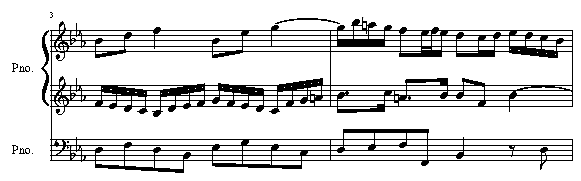
\includegraphics[width=400px]{../images/bwv05225_excerpt.pdf}}
\caption{Excerpt of Bach's BWV 05225}
\label{ims:be05225}
\end{figure}

Figure \ref{ims:be05225} shows the music sheet of an excerpt of Bach's BWV0525 Sonata using modern notation. 

The musical data from musical pieces need to have a proper representation in order to be used by a machine learning algorithm.

In \cite{Eck2002} Eck a form of 12-bar blues was used with 8 notes per bar. 
He used the following representation for the \acs{LTSM} system:
\begin{enumerate}
\item 12-bar musical pieces were used
\item 8 notes per bar were used
\item The same chords were used between songs, see figure \ref{ims:eckchords}
\item The melody notes were built using the pentatonic scale
\item The neural network inputs indicate whether a certain note is on or off
\end{enumerate}

A melody would be represented differently in a linear genetic algorithm.
A simple melody consisting only of a few notes could be represented as seen in figure \ref{ims:ga_melody}. Note the duration of a note is not defined and could be consider fixed.

However it might be preferable to encode more events such rests, chords, dynamics, note duration and so on.

Tree based representations are found in genetic programming \cite{Langdon2008}. Minsky has argued that tree representation is more suited to music as it mimics the hierarchical structure that is found in music \cite{Minsky1992}.

A melody could be represented in tree form as seen in figure \ref{ims:gp_melody}. The bottom leaves denote the pitch and duration. The higher level nodes perform operations.


\begin{figure}
\centering
\begin{minipage}{.5\textwidth}
  \centering
  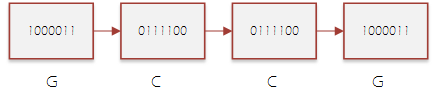
\includegraphics[width=180px]{../images/ga_melody.png}
  \caption{Simple melody represented as a bit string}
\label{ims:ga_melody}
\end{minipage}%
\begin{minipage}{.5\textwidth}
  \centering
  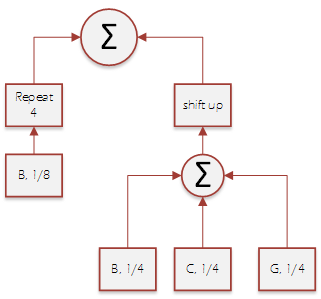
\includegraphics[width=180px]{../images/gp_melody.png}
  \caption{Simple melody represented in tree form}
\label{ims:gp_melody}
\end{minipage}
\end{figure}

\begin{figure}
\centerline{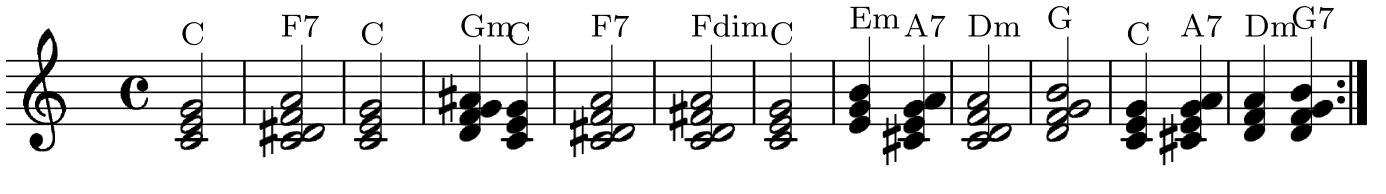
\includegraphics[width=400px]{../images/eck_chords_training.png}}
\caption{Training chords used in \cite{Eck2002}}
\label{ims:eckchords}
\end{figure}

Johanson and Poli employ several different operators including mirroring, concatenation, repetition and mirroring \cite{Johanson1998}

Tree based representations do not have a fixed size, as is commonly found in linear genetic representations. Care must be taken to not let the structure become too large. This is typically done by specifying the maximum depth of the tree.

%********************************************************************************************************
%********************************************************************************************************
%********************************************************************************************************

\chapter{Music composition algorithms} \label{chap:comp_algo}

\section{Hidden Markov Models} \label{sec:hmm_backround}

\begin{figure}[ht!]
\center
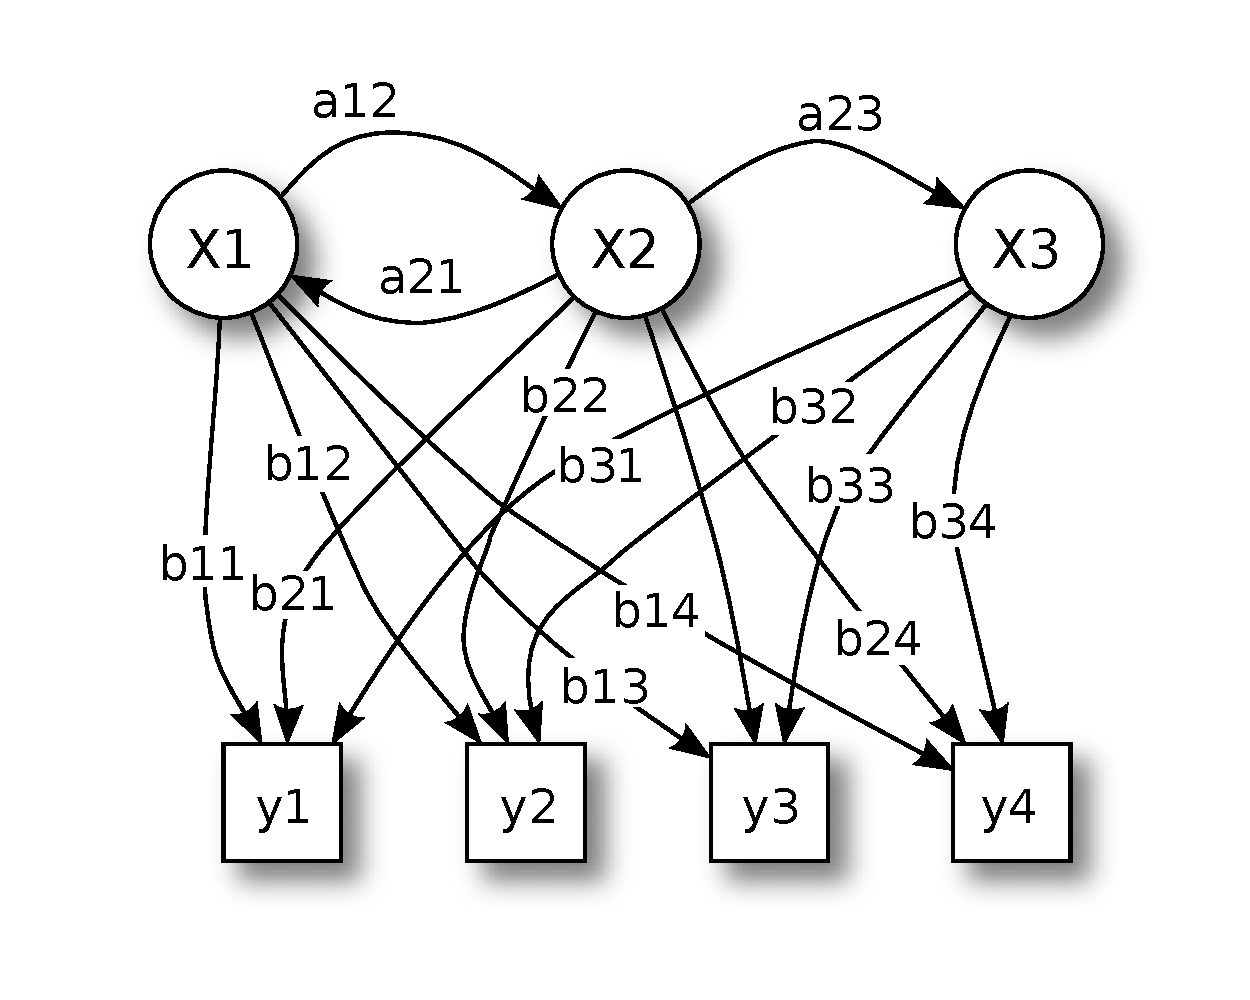
\includegraphics[width=250px]{../images/HiddenMarkovModel.pdf}
\caption{Example of a Hidden Markov Model}
\label{ims:hmm_example}
\end{figure}

\subsection{Introduction}



\ac{HMM} are stochastic methods that are used to model sequential data such as speech and gesture recognition. Both the underlying process which is hidden is stochastic and the observable process. Only a first order hidden markov model will be considered.
%TODO insert citation
Under the Markov property the next state is only dependent on the current state of the system. Such states may not be known and may be hidden from the observer as only the output values are observable. When a event is generated from a state, the model moves into a new state based on its transition probabilities. The term hidden is commonly used to indicate that many different state sequences can generate the same observed sequence of events.

The \ac{HMM} is formally defined by the triple:
\[\lambda = (A,B,\pi) \]
where A is the transition matrix, B the emission matrix and $\pi$ the initial state vector. Let $S$ be the set of states, $V$ the set of observations, $Q$ a fixed state sequence of length $T$ and $O$ a corresponding observation sequence.
The transition probabilities are then given by:
\[ A = P(q_t = s_j | q_{t-1} = s_i) \]
and the emission probabilities are given by:
\[ B = P(o_t = v_k | q_t = s_i) \]
and the initial state probabilities by:
\[ \pi = P(q_1 = s_i) \]

Given a sequence of observations we want to compute the probability of an observation sequence given the model.

The probability of the observation sequence $O$ for a state sequence is given by:
\[ P(O|Q,\lambda) = \prod^T_{t=1} P(o_t | q_t,\lambda) \]
The probability of the state sequence is simply a product of the state path:
\[ P(Q|\lambda)= \pi_{q_1}a_{q_1 q_2} \cdots a_{q_{T-1} q_T} \]
Thus the probability of the observations given the model can be calculated by:
\[ P(O|\lambda) = \sum_Q P(O|Q,\lambda) P(Q|\lambda) \]

The forward algorithm calculates this efficiently by caching previous calculations.

\subsection{Training}

A variety of learning algorithms exist which compute the structure of the model and also calculate the emission and transmission matrices. The Baum-Welch is a unsupervised learning algorithm which re-estimates the parameters $(A,B,\pi)$. The training problem can be solved in terms of joint events and state variables \cite{Baum1970}.

The joint variable $\xi_t(i,j) = P(q_t = S_i, q_{t+1} = S_j|S, \lambda)$ is given by:
\[ \frac{\alpha_t (j) a_{ij} b_j (O_{t+1}) \beta_{t+1}(j) }{\sum_{k=1}^N \sum_{l=1}^N \alpha_t (k) a_{kl} b_l (O_{t+1}) \beta_{t+1}(l) } \] 

The state variable $\gamma_t(i) = P(q_t = S_i | O, \lambda)$ is given by:
\[ 
\gamma_t(i) = \frac{\alpha_t (i) \beta_t(i)}{\sum_{j=1}^N \alpha_t (j) \beta_t (j)}
\]

Upon which the parameters can be updated. The updated state transition probability is then given by:
\[a'_{ij} = \frac{\sum^{T-1}_{t=1} \xi_t (i,j)}{\sum_{t=1}^{T-1} \gamma_t (i)} \]
The updated emission probability is given by:
\[ b'_j (k) = \frac{\sum^T_{t=1,o_t = v_k} \gamma_t (j)}{\sum^T_{t=1} \gamma_t (j)} \]
The updated initial probability by:
\[ \pi'_i = \gamma_1 (i) \]

\subsection{Composition}
\acs{HMM} have been applied with some degree of success to music composition. A system has been developed for producing a counterpoint line to a cantus firmis in the style of Palestrina \cite{Farbood2001}. Another approach utilizes a \ac{HMM} for chorale melody harmonization \cite{Allan2004}.



\section{Markov Chains} \label{sec:markov_backround}
\subsection{Introduction}
A Markov Chain is a stochastic model describing a sequence of events. The Markov Chain has the property that the probability of the next state depends only on the current state of the chain.
\[ \Pr(X_n | X_1, X_2, \ldots, X_{n-1}) = P(X_n | X_{n-1})  \]

\begin{figure}
\center
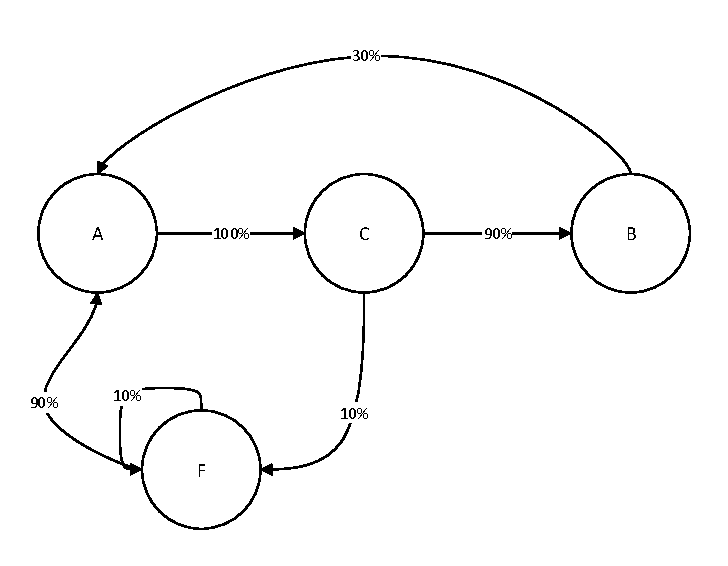
\includegraphics[width=250px]{../images/markov_chain_example.pdf}
\caption{Example of a Markov Chain}
\label{ims:markov_chain_example}
\end{figure}

Figure \ref{ims:markov_chain_example} is an example of a Markov Chain. For each state there is a probability of proceeding to the next state. For example if the current state is F, there is a $10\%$ chance of the next state being F again, and a $90\%$ chance of the next state being A.

A Markov Chain can have a order. For a simple note such as figure \ref{ims:markov_chain_example} if the current note is B then the note $A$ has a $30\%$ chance of being next. This is a first order Markov Chain.  A more complex chain of order 2 could have the current state being composed of two notes. Thus the next note is dependent on the previous two notes. A N-th order Markov chain can be represented by a transition matrix, which corresponds to a N+1 dimension probability table.

For a Markov Chain of order $m$ the following holds:
\[
\Pr(X_n=x_n\mid X_{n-1}=x_{n-1}, X_{n-2}=x_{n-2}, \dots , X_1=x_1)
\]
\[\quad = \Pr(X_n=x_n\mid X_{n-1}=x_{n-1}, X_{n-2}=x_{n-2}, \dots, X_{n-m}=x_{n-m})
\]
For $n > m$

\subsection{Composition}
Markov Chains must be derived from existing music and generate output of the same style as the input. This reduces the compositional value and novelty however it suits the purpose of generating music in a specific style \cite{Jarvelainen2000}.

Context models such as Markov Chains have several advantages that are useful in algorithmic music composition \cite{Conklin2003}:
\begin{itemize}
\item Events can be predicted from preceding events.
\item Context models are fast and efficient data structures can be used.
\item Most context models are straightforward to generate new music with.
\end{itemize}
%\section{Harmony Search Algorithm}
%Music pieces have been composed using a behavior-inspired evolutionary algorithm, harmony search (HS). The HS algorithm mimics behaviors of music players in an improvisation process, where each player produces a pitch based on one of three operations (random selection, memory consideration, and pitch adjustment) in order to find a better state of harmony which can be translated into a solution vector in the optimization process. When HS was applied to the organum (an early form of polyphonic music) composition, it could successfully compose harmony lines based on original Gregorian chant lines.

%****************************************************************************************************

\section{Neural Networks}
\subsection{Background}
\begin{figure}[h!]
\center
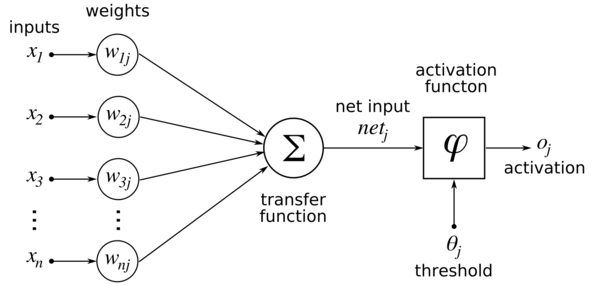
\includegraphics[width=300px]{../images/ANN_neuron.png}
\caption{Model of artificial neuron}
\label{ims:ANN_neuron}
\end{figure}
\begin{figure}
\centerline{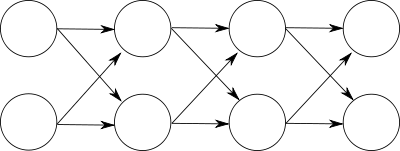
\includegraphics[width=200px]{../images/ANN_feedforward.png}}
\caption{Figure of ANN in feed-forward topology}
\label{ims:ANN_FF}
\end{figure}
An artificial neural networks consists of layers of artificial neurons\footnote{neurons are commonly referred to as units} (see figure \ref{ims:ANN_neuron}) that are connected to each other in a certain topology \cite{bishop1995neural}.

Figure \ref{ims:ANN_FF} shows a multilayer ANN in feed-forward topology. The first layer is referred to as the input layer, the right-most layer is referred to as the output layer, the layers in between the input layer and the output layer are known as hidden layers.

Neurons have a number of inputs which are summed into an activation function. The activation function provides the output of a neuron.
In figure \ref{ims:ANN_neuron} we have
\[ o_j = \varphi\left(\sum^{n}_{i=1} x_i w_{ij}\right)  \]
A common activation function is the continuous sigmoid function given by
\begin{equation} \varphi(t) = \sigma(t) = \frac{1}{1+e^{-\beta t}}  \label{eq:sigmoid}\end{equation}
where $\beta$ is the slope parameter.
The derivative of the sigmoid function is easy to obtain and is given by:
\begin{equation} \frac{\sigma(t)}{dt} = \sigma(t)(1-\sigma(t))\label{eq:sigmoidd}\end{equation}
for $\beta=1$

In order to determine weights for a two-layer neural network we need to minimize the error between the output of the neural network and the given target value for a set of inputs. 

Thus for the output neurons we have
\begin{equation} E(\vec{w}) = \frac{1}{2} \sum_{d \in D}(t_d - \sigma_d)^2 \label{eq:error} \end{equation}\
where $D$ is the set of training examples and $t_d$ is the target output for training example $d$ and $o_d$ is the output of the artificial neuron for training example $d$
We need to minimize equation \ref{eq:error}.
Obtaining the derivative of $E$ with respect to $w_i$ yields:
\[ \frac{\partial E}{\partial w_i} = \sum_{d\in D}(t_d - o_d)(-x_id) \]
where $x_{id}$ is the input for component $x_i$

Gradient descent is a optimization algorithm that takes steps proportional to the negative of the gradient. This we update the weights by:
\[\vec{w} \leftarrow \vec{w} - \eta \nabla E(\vec{w}) \]
Applying the gradient descent algorithm we obtain a weight update rule of
\[ w_i \leftarrow w_i + \eta \sum_{d \in D} (t_d - o_d) x_{id} \]
For a multi layer network with multiple output units the back propagation algorithm needs to be used.
The error needs to be summed over all the network output units
\[E(\vec{w}) = \frac{1}{2} \sum_{d \in D} \sum_{k \in \text{outputs}} (t_{kd} - \sigma_{kd})^2 \]

The back-propagation algorithm to determine the weights of a feed-forward neural network is given in appendix \ref{chap:app_algo}


\subsection{Composition}
Neural networks have been used in music classification, in genetic algorithms as fitness functions and more complex neural networks have even been used in algorithmic music compositions.

Simple feed-forward neural networks do not contain a mechanism to remember past history.  
\\
\\
In \cite{mozer1994neural} Mozer created a recurrent connectionist neural network \textbf{CONCERT}\footnote{CONCERT - connectionist composer of ERudite tunes}\footnote{The ER may also be read as ERratic or ERsatz}.
The system works as follows:
\begin{itemize}
\item The network is trained on sample melodies from which it learns melodic and phrase constraints
\item Representations of pitch, duration and harmonic structure are included that are based on psychological studies of human perception, based on Laden and Keefe's work \cite{laden1989representation}
\end{itemize}
The system yielded good results on simple structured artificial sequences however the system performed poorly on natural music\footnote{One critic described the resultant melodies as compositions only a mother could love}. Mozer described the system as lacking musical coherency \cite{mozer1994neural}. Furthermore the system performs poorly as the length of the pieces increases.

Mozer stated the reason for failure is likely due to the \ac{RNN} not being able to track more distant events that build global structure \cite{mozer1994neural} however a \ac{LSTM} recurrent network is able to achieve this goal \cite{Eck2002}.
\\
\\
In order to solve the problem of global structure Douglas and Jurgen attempted to use a \ac{LSTM} network to compose musical pieces \cite{Eck2002}. In this attempt the network was successfully able to learn a form a blues music and stay close to the relevant structure.
The system used cross entropy as the error rate:
\[
E_i = -t_i \ln(y_i) - (1-t_i)\ln (1-y_i) \]
where $y_i$ is the output activation and $t_i$ the target value for the $i-th$ output unit.
The topology of the network was arranged as follows:
\begin{enumerate}
\item Four cell blocks are connected to the input units for chords
\item The last four cell blocks are connected to the inputs units for melody
\item Chord cell blocks have recurrent connections to themselves and melody cell blocks
\item Melody cell blocks have recurrent connections to other melody cell blocks
\item Output units for chords are connected to cell blocks for chords and to input units for chords
\item Output units for melody are connected to cell blocks for melody and to input units for melody
\end{enumerate}
The underlaying chord structure was kept fixed.

The results indicate that a \ac{LSTM} network is able to compose with both local- and global structure from a set of training data \cite{Eck2002}.


\subsection{Conclusion}

Simple feed-forward neural networks do not have the functionality to remember past history and thus do not have the capability to evaluate repetitive rhythmic patterns.

Recurrent neural networks are able to encode temporal information though initial investigation by Mozer lead to limited success as compositions lacked global structure. 

Further investigations by Douglas and Jurgen indicated that \ac{LSTM} networks are able to compose with local and global structure.

%****************************************************************************************************
\section{Genetic Algorithms}
\subsection{Background}

Genetic Programming, not to be confused with evolutionary or genetic algorithms is a evolutionary algorithm based methodology to find computer programs that perform defined tasks by simplistically mirroring biological evolution.
The more fit programs carry on their chromosomes into future populations. Fitness is rated by a fitness function. Other genetic operators such as recombination and crossover are also usually applied. 
These evolved genetic programs are usually represented in tree form. Figure \ref{ims:gpt} indicates the function $ (2.2) - (\frac{X}{11}) + 7\cos(Y)$ written in tree form.
\begin{figure}[!bh]
\centerline{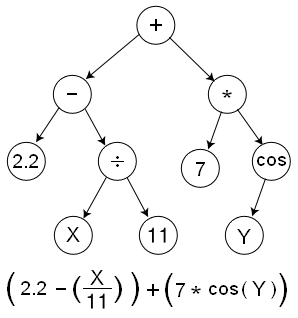
\includegraphics[width=150px]{../images/gpt.png}}
\caption{Figure of a example genetic program tree}
\label{ims:gpt}
\end{figure}

A genetic algorithm consists of the following components:
\begin{enumerate}
\item Representation for chromosomes\footnote{Also commonly referred to as an individuals}
\item Initial population of chromosomes
\item A set of genetic operators to alter the population
\item A fitness function to assess the fitness of an individual
\item A selection method to determine which individuals in a population survive
\end{enumerate}
The algorithm proceeds as follows:
\begin{enumerate}
\item Initial population is randomly generated
\item The fitness of each individual is assessed
\item Individuals are selected to which genetic operators are applied, e.g.
\\Two parents are selected to generate a new child with crossover
\\Random mutation occurs in individual
\item Various forms of selection are available that determine which individuals will be in the next generation
\end{enumerate}

Genetic operators are used to generate diversity A genetic algorithm has a fixed set of genetic operators. Operators may include:
\begin{itemize}
\item Reproduction - A parent from the population is carried over to the next generation
\item Crossover - genotype of both parents are combined using different procedures
\item Mutation - A single mutation is applied to a chromosome at a set mutation rate
\end{itemize}

The choice of a fitness function is a big problem when using a genetic algorithm to compose music \cite{Wiggins1998,Matic2010}. There is no objective method to rate whether a melody is good or bad \cite{Lo2012}. 
Traditionally when posed against such tasks the fitness function is provided interactively by the user, i.e. the user rates whether the piece is good or bad

The interactive GA approach is an approach to the fitness function where a human interactively rates the quality of a composition (fitness). A well known software that utilizes a neural network and a interactive interaction for a fitness function is GenJam \cite{Biles1996}. The drawback of having the user interactively evaluate the fitness of individuals is that it is time consuming and poses a processing bottleneck \cite{Eck2002}

Selection is the choice of which individuals will be chosen for the next generation. Selection concerns the reproduction and crossover operators. Some methods of selection include: 
\begin{itemize}
\item Roulette wheel selection - chance of individual being chosen is proportional to fitness
\item Tournament selection - tournament is staged between two individuals to determine which one gets selected\footnote{This is tournament selection in its simplest form}.
\item Elitist selection - commonly the best few individuals are kept unchanged but are eligible to be selected as parents.
\end{itemize}

\subsection{Composition}

Genetic algorithms have already been used in a variety of work in algorithmic music composition. Some of these include:
\begin{itemize}
\item Thematic bridging \cite{Horner1991}
\item Composition systems using \acsp{IGA} \cite{1412045}
\item \acsp{IGA} to improvise jazz solos \cite{Biles1996, Biles1994}
\item Integration between interactive genetic algorithms and genetic programs \cite{Tokui2000}
\item Hybrid approaches employing statistical, connectionist and evolutionary elements \cite{Manaris2007}
\item Various work into different fitness functions
\end{itemize}

In Alfonseca's system the generated musical pieces had the style of well-known authors even when the fitness function only took relative pitch envelope into account and all generated note lengths were of fixed duration \cite{Alfonseca2007}.
\\
\\
Thematic bridging is the application of an initial music pattern to a final pattern over a specified duration \cite{Horner1991}. In this approach Horner modified or reordered elements in a music pattern through various operations. For example:

Given the initial note pattern of:
 \begin{verbatim}Gb Bb F Ab Db \end{verbatim}
and a final note pattern of:
\begin{verbatim}F Ab Eb \end{verbatim}
the musical output could be:
\begin{verbatim}Gb Bb F Ab Bb F Ab Gb Bb F Ab Eb F Ab F Ab Eb \end{verbatim} by means of various operations such as mutation, rotation, deletion and so on.
For thematic bridging a composite fitness function was used which rates how close the developed pattern matches the final pattern and whether the ordering of the elements are correct 
\\
\\
Similarly a system of variations was developed Jacob that proceeds as follows \cite{Jacob1995}:
\begin{enumerate}
\item Define a primary set of motives
\item Compose phrases by layering and sequencing new motives
\item New motives are created by variations of motives already in the phrase
\item Phrases are combined together
\end{enumerate}
Jacob's system had a human judge evaluate the individual chromosomes. 
\\
\\
\ac{NCD} has also been commonly used as a fitness function, for more information about the normalized compression distance see sections \ref{sec:class_ncd} (in music classification) and \ref{sec:ncdfitness} (as a fitness function).
Alfonseca proposed the following genetic algorithm scheme for composing melodies \cite{Alfonseca2007}:
\begin{enumerate}
\item Define a set of $M$ musical pieces for a guide set $G$
\item Encode both the guides and individuals in the population as pairs of integers where the first integer represents the note interval and the second the length as a multiple of the minimum unit of time.
\item See eq. \ref{eq:ncdfitness} on page \pageref{eq:ncdfitness} for the fitness function used
\item The 16 lowest fitness genotypes of every generation is removed
\item The 16 highest fitness genotypes of every generation are paired by means of genetic operations.
\end{enumerate}


\subsection{Conclusion}
There are a variety of alterations on genetic algorithms and genetic programs, however evolutionary algorithms in general are a viable means to compose music.

The encoding of a musical piece as a chromosome affects the interactions of the genetic operators on the musical piece and most authors encode the problem differently.

It is important to restrict the domain of problem otherwise the search space for the genetic algorithm may be too large \cite{Jacob1995}. Most of the studies listed in this document had restricted goals.
For example, using only two octaves for the notes significantly reduces the size of the search space and many real melodies comply with it \cite{Alfonseca2007}

The fitness function is an important part for having the genetic algorithm result to good melodies. See section \ref{sec:chapfitness} for insight literature has on fitness function for evolutionary algorithms.
The representation of melodies for the algorithm is arguably just as important.

For this project the focus is on evolutionary and learning algorithms and as such other procedural means of music composition will be neglected. 

Fitness functions for genetic algorithms are considered in chapter \ref{sec:chapfitness}. Possible music classification algorithms will also be investigated as they can serve as fitness functions.


%********************************************************************************************************
%********************************************************************************************************
%********************************************************************************************************

\chapter{Music classification} \label{sec:music_class}
\section{Introduction}
In this section we will investigate methods of music classification. If some algorithm is a good method to rate the closeness of a song to a genre or style then it may also serve as a good fitness function for a evolutionary algorithm.
%\section{Feature set patterns}
%Melody classification using patterns
%Darrell Conklin
%Abstract. A new method for symbolic music classification is proposed,
%based on a feature set pattern representation. An ensemble of sequential
%patterns is used to classify unseen pieces using a decision list method.
%On a small corpus of 195 folk song melodies this method achieves a good
%classification accuracy of 77\%, though with only a 43\% recall rate.


\section{Normalized Compression Distance} \label{sec:class_ncd}
\subsection{Background}
The Kolmogorov complexity of piece of text is the measure of the computable resources needed to specify the text. The complexity of a string is the length of the shortest possible description of the string in a fixed universal description language \cite{Kolmogorov1998387}.

The information distance between two string $x$ and $y$ is defined as the length of the shortest program $p$ that can compute $x$ from $y$ and $y$ from $x$
The length of $p$ can be expressed using Kolmogorov complexity \cite{681318}:
\[ |p| = \max\{K(x|y), K(y|x)\}  \]

The information distance $p$ is a absolute measure. A more useful similarity metric is one that expresses the distance in relative terms. 
The \ac{NID} is given by \cite{1362909} : 
\[ \text{NID}(x,y) = \frac{\max\{K(x|y),K(y|x)\}}{\max\{K(x),K(y)\}} \]

The concept of \ac{NID} is important, however it is not computable. 
An approximation of the normalized information distance is commonly used.  $K(x)$ is approximated by $Z(x)$ where $Z(x)$ is the binary length of a data $x$ compressed by a compressor $Z$.
\[NCD(x,y) = \frac{Z(xy) - \min\{ Z(x), Z(y) \}}{\max\{ Z(x), Z(y) \}} \]
where $Z(xy)$ is the length of $x+y$ compressed by $Z$. 
Any good compressor may be used for $Z$ such as 
\begin{itemize}
\item Gzip
\item Bzip2
\item Lempel-Ziv and its variations
\end{itemize}
\subsection{Literature}
Normalized compression distance has been used in a variety of cases. It has been used in applications of general clustering and classification of data in arbitrary domains. This includes music classification \cite{1412045}.

Cilibrasi and Vitiyani used the Normalized Compression Distance to approximate the Kolmogorov Distance between different musical pieces as a method to compute clusters of music \cite{1412045}. The \ac{MIDI} files were pre-processed such that when two notes occur at the same time only the note with the highest pitch is kept. The music was represented as a string and the distances between different musical pieces was computed.


Ctaltepe, Sonmez and Adali used the normalized compression distance and used it to classify music pieces using k-nearest neighbors \cite{Cataltepe2005}. 
The training data has a label associated. The closest $k$ training data (by \ac{NCD}) to a song is obtained and the most frequent label in the $k$ set is used to classify the musical piece. 
Ctaltepe Sonmez and Adali found that the distance measure works better when more training data is available and the performance is dependent on how the input data is pre processed. 
The best results were obtained when the midi files were sampled at $1$ms and the $k=1$ nearest neighbor identification was used. 
The music was represented in the following format: outputting the first note and then the difference in pitch between consecutive notes. Using the above means a classification accuracy of $79\%$ was achieved on 57 midi files.

Li and Sleep have also found that the 1-nearest neighbor with a Lempel-Zip compressor outperformed more complex statistical methods and compressors. Using relative pitch intervals in the music representation outperformed using absolute pitches. A performance of $92.35\%$ was obtained \cite{Ling2004}.
The midi files were organized into four categories Beethoven (302 files), Haydn (261 files), Chinese (80 files) and Jazz (128 files). The dataset is unbalanced and the study does not make it clear which partition of the dataset was used as training samples and what partition was used for verification.

In \cite{Alfonseca2007, Alfonseca:2005:ECM:1981094.1981161, Ling2004,Alfonseca2006} it was found that the normalized compression distance serves as a promising fitness function for genetic algorithms for automatic music generation. Thus \ac{NCD} may be viably used as a fitness function for a genetic algorithm and as a metric to help classify music.

\section{Neural Networks}
McKay investigate using K-nearest neighbor techniques and artificial neural networks in order to classify \ac{MIDI} music by genre.
He included some of the following metrics as input to the neural network \cite{Mckay2004}:
\begin{itemize}
\item Number of notes - standard deviation of number of notes activated in each channel
\item Note duration - standard deviation of total duration of notes
\item Dynamics - standard deviation of average volume of notes
\item Melodic Intervals - average melodic interval
\item Simultaneity - average number of notes that are played concurrently
\item Note density - average number of notes per second
\item Average time between attacks - average time between note activations
\item Initial tempo - tempo in beats per minute
\item Pitch variety - number of pitches used at least once
\item Most common pitch class - Most common pitch divided by number of possible pitches
\end{itemize}
The complete set can be found in Mckay's dissertation \cite{Mckay2004}
Using the complete list of metrics neural networks had a success rate of $83\%$.
%********************************************************************************************************
%********************************************************************************************************
%********************************************************************************************************

\chapter{Fitness Functions}\label{sec:chapfitness}

%********************************************************************************************************

\section{Introduction}
In this section we will briefly review some functions that may be used as a fitness function for a genetic algorithm.

%Some other functions that may be used, but with mixed results are identified in section \ref{sec:other} briefly.

Algorithms that help classify music could possibly be used as fitness functions, as this would rate the similarity of the evolved piece of music to a genre or style. These algorithms are found in section \ref{sec:music_class}.
If work has been done that has used the music classification algorithm as a fitness function it will be listed in this section.

Fitness functions can be categorized as follows:
\begin{itemize}
\item Interactive - The user provides the fitness of a piece of music
\item Expert systems - The musical fitness is assigned according to best practices commonly studied in music theory
\item Learning based functions - Fitness functions that learn from previous data
\end{itemize}

Learned fitness functions are sensitive to input data and the selection of features is a difficult task \cite{Dostal2013}, however the focus here is on learning algorithms.
%********************************************************************************************************


\section{Zipf's law} \label{sec:zipfs_fitness}
Zipf's law states that the frequency of an event is inversely proportional to its statistical rank, that is:
\[ f \propto r^{-a} \]
where $f$ is the frequency of occurrence of a particular event and $r$ is the statistical rank. $a$ is close to $1$.
Zipf's law can also be stated as:
\[ P(f) \approx \frac{1}{f^n}\]
where $P(f)$ denotes the probability of an event of rank $f$ and $n$ is close to $1$

One can determine whether melodic intervals follow Zipf's law by counting the melodic intervals in a piece. The result is usually plotted on a logarithmic scale and is known as a rank-frequency distribution

Zipf found evidence for the theory in music. An analysis of Mozart's Bassoon Concerto in Bb Major revealed an inverse relationship between the length of intervals between repetitions of notes and the frequency of their occurrence \cite{zipf1949human}.

Several other different rank frequency distributions can be obtained for a musical piece.
These include \cite{Manaris2005}:
\begin{itemize}
\item{Pitch}{ - distribution of \ac{MIDI} pitches}
\item{Chromatic tone}{ - distribution of 12 chromatic tones}
\item{Duration}{ - note durations}
\item{Melodic interval}{ - distribution of melodic intervals}
\item{Melodic bigrams}{ - distribution of adjacent melodic interval pairs}
\end{itemize}
Linear regression is performed to obtain the slope of the distribution. The coefficient of determination $R^2$ is also computed in order to determine how well the slope fits the data.

\begin{figure}
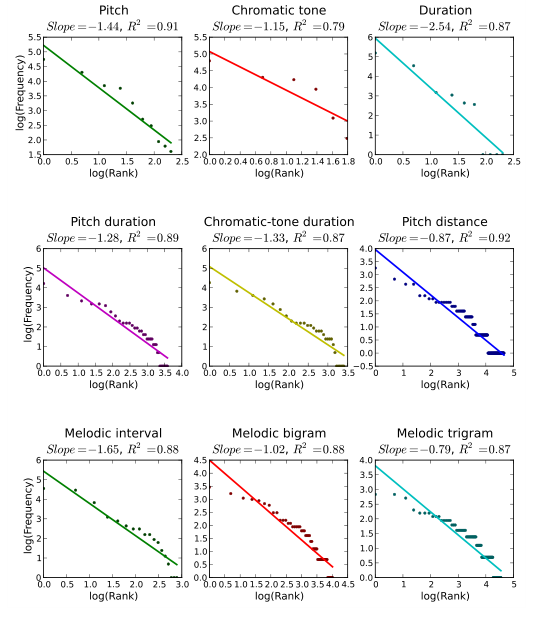
\includegraphics[width=400px]{../images/zipf_letitbe.png}
\caption[Rank frequency distributions for Let It Be]{Rank frequency distributions and slopes of different metrics for The Beatles' Let It Be
\footnotemark}
\label{ims:zipf_letitbe}
\end{figure}
\footnotetext{Figure generated by Jensen for his thesis \cite{Dostal2013}}


Figure \ref{ims:zipf_letitbe} plots the rank frequency distributions of various metrics for the Beatles' song Let It Be. The figures were generated by Jensen for his thesis \cite{Dostal2013}. The metrics can be seen to follow a Zipfian distribution. Results by Manaris also indicate that most music pieces display near Zipfian distributions \cite{Manaris2005}.

Zipf-based metrics capture essential parts of scaling properties in music. These metrics indicate that music follows a distribution balanced between near-zero slope and steep negative slope. Different styles of music have different slopes.
There exists also a correlation between Zipf metrics and human preference \cite{Manaris2005}.

Jensen used a Gaussian to define the target fitness as \cite{Dostal2013}:
\[f_m(a,b) = e^{(\frac{b-a}{-\lambda})^2} \]
where $a$ is the metric slope of an evolved piece of music, $b$ is the target slope and $\lambda$ is the tolerance

Since there are several metrics for a given piece of music the fitness function should incorporate these.
Jensen used the weighted sum of several metrics.  
\[f(\vec{a}, \vec{b}) = \sum_{i=1}^{N} w_i f_i(a_i, b_i) \]

Jensen has found that Zipf metrics can be used to evolve pleasant music using a tree-based representation, however the majority of the evolved melodies were unpleasant \cite{Dostal2013}. Zipf metrics only capture the scaling properties of distributions and ignore the musical events that account for different frequencies. Zipf's law neglects musical content and can be seen as knowledge weak.
Jensen concluded that the Zipf metrics are insufficient for musical fitness alone.

Manaris had more success with Zipf metrics however he used them as input to an artificial neural network to evaluate the fitness of melodies, however Manaris states it is wiser to use the fitness function in a partially interactive system \cite{Manaris2005}

%********************************************************************************************************

\section{Cosine Similarity}
In Information Retrieval cosine similarity is commonly used to asses the similarity of two documents:
\[\text{sim}(\vec{A}, \vec{B}) = cos\theta = \frac{\vec{A} \cdot \vec{B}}{|\vec{A}||\vec{B}|} \]
where $\vec{A}$ and $\vec{B}$ are two document vectors

In order to rate the similarity between music scores features such as pitches and melodic intervals are used.

As with Zipf's law the fitness is the weighted sum of similarity measures:
\begin{equation}f(\vec{A_1}, \ldots, \vec{A_n}; \vec{B_1}, \ldots, \vec{B_n}) = \sum^N_{i=1} w_i f_i (\vec{A_i}, \vec{B_i}) \label{eq:fitcosfit} \end{equation}
The fitness function rates the fitness of the evolved individual with a target piece.

Jensen conducted multiple experiments using the fitness function in equation \ref{eq:fitcosfit}. The metrics covered indicate the frequency of certain events. At first only a single metric was included and thereafter multiple metrics. As more metrics were included the evolved melodies became more similar to the target piece. More pleasant melodies were evolved when the target piece was The Beatle's Let It Go than Mozart's Piano Sonato No. 16. There was no correlation between melody and rhythm.
Metrics included for the fitness function were:
\begin{itemize}
\item Pitch
\item Chromatic tone
\item Melodic interval
\item Melodic bigram
\item Rhythmic interval
\item Rhythmic bigram
\end{itemize}
Jensen concluded that the results obtained by the cosine similarity fitness function were more pleasant than those obtained by Zipf's law as Zipf's law rates music on scaling properties only \cite{Dostal2013}.

%********************************************************************************************************


\section{Neural Networks} \label{sec:ANN_fitness}
Different forms of networks have been used as a fitness function for evolutionary algorithms.
Some of these include:
\begin{itemize}
\item Adaptive resonance theory neural networks using binary classification patterns \cite{Burton97geneticalgorithm}
\item Recurrent neural networks
\item Cascade correlation neural network designed to reduce GenJam bottleneck \cite{Biles1996}
\end{itemize}

Some common problems with neural networks as fitness functions is that they require a lot of time to be trained, require a good representation for a set of inputs to map to an output and the structure of the neural network is fixed after training \cite{Burton97geneticalgorithm}. 

In \cite{Biles1996} Biles tried to design a cascore neural network to rate musical scores. Since a neural network outputs fitness based on the input parameters the choice of input metrics are important.
Metrics that included the number of new note events in a measure, the number of unique new note events, the size of the maximum interval, the number of changes in a direction between adjacent notes failed to capture the fitness for the \ac{ANN} \cite{Biles1996}.

Biles argues that the reason for this is that humans listen to music in more complex ways and that simple statistical measures fail to capture this. Zipfs law, which only captures the scaling properties of music also yielded poor results as a fitness function for similar reasons \cite{Dostal2013} (See section \ref{sec:zipfs_fitness}). 
\\
\\
An \ac{ART} network has been used as a fitness function whereby a \ac{GA} utilizes clustered representations of rhythm styles to interactively generate rhythm patterns to according to a certain style \cite{Burton97geneticalgorithm}.

An adaptive resonance theory network utilizes unsupervised learning and clustering algorithms to recognize patterns. New clusters are created if a pattern cannot be associated with existing clusters. Another characteristic of \ac{ART} networks is that new training does not cause loss or corruption of old training data \cite{carpenter2010adaptive}

A ART1 network clusters binary vectors. The basic structure of an ART1 network involves (See figure \ref{ims:ANN_art}) :
\begin{enumerate}
\item Input processing field - $F1$
\item Cluster units - $F2$
\item Mechanism to control degree of similarity of patterns in the same pattern
\item weighted bottom-up connections between $F1$ and $F2$ layers
\item weighted top-down connections between $F2$ and $F1$ layers
\end{enumerate}

\begin{figure}
\centering
\includegraphics[width=300px]{../images/ann_ART.png}
\caption{Figure of ART ANN topology}
\label{ims:ANN_art}
\end{figure}

Burton had the \ac{ART} network fitness function operate as follows \cite{Burton97geneticalgorithm}:
\begin{enumerate}
\item Each individual in the population is an input to the \ac{ANN}
\item The network determines the winning cluster
\item The degree of similarity between the individual and the cluster is determined
\item If the degree of similarity is above a certain threshold the individual is added to the cluster
\item If no clusters match the individual closely enough a new cluster is created
\item Fitness is assigned as a degree of similarity to a cluster. 
\end{enumerate}

NEUROGEN is another attempt at using a neural network as a fitness function to compose small diatonic, western, four part harmony compositions.
The system has shown limited success however it was able to produce 4 bars of music \cite{gibson1991neurogen}.
\\
\\
Chen used a \ac{SRN} with composition rules on tonality and rhythm as a fitness function for a \ac{GA} \cite{Chen2001}. The simple recurrent network has an input layer that represents a measure at time $T$ with the output layer representing the measure at time $T+1$.
A recurrent network is used as a single step predictor to compose music. The network predicts notes at $T+1$ using the notes at time $T$. After the network has been trained it can be seeded with inital values to generate novel compositions.
The following constraints were used:
\begin{enumerate}
\item Pitch diversity constraint - number of measures with unique pitch sequences
\item Rhythmic diversity constraint - number of measures with unique signatures
\item Measure density constraint - ratio of number of notes to maximum notes
\item Pentatonic pitch class constraint - number of notes that belong to pentatonic pitch class
\item Cell structure - ratio number of times cell pattern occurs to maximum number of patterns 
\end{enumerate}
The system was able to generate melodies with systematic structure however it lacks global structure. Individual measures sound pleasant and diverse however there is a lacking structure as a whole
%********************************************************************************************************

\section{Normalized Compression Distance} \label{sec:ncdfitness}
As noted in section \ref{sec:music_class} the Normalized Compression Distance has been used to help classify music genres. However Normalized Compression Distance has been explored as a possible fitness function for evolutionary algorithms \cite{Alfonseca2007,Alfonseca:2005:ECM:1981094.1981161,Alfonseca2006}

The fitness function used by Alfonseca et. al for an individual $x$ and a guide set $G$ was defined as \cite{Alfonseca2006}: 
\begin{equation}f(x) = \left( \sum_{g_i\in G} \text{NCD}(x,g_i) \right)^{-1} \label{eq:ncdfitness} \end{equation}
Where $g_i$ is a guide in guide set $G$ containing $M$ musical pieces and $x$ is the set of differences between consecutive notes.

Alfonseca encoded the chromosomes as $N$ vectors containing a pair of integers. The first integer denotes the note interval and the second represents the length as a multiple of the smallest unit of time \cite{Alfonseca2007}.

%********************************************************************************************************

\section{Interactive fitness functions} \label{sec:iga}
Genetic algorithms which employ user interaction as a means of rating the fitness of are known as \acfp{IGA}.

Unehara constructed a system that composes 16-bars music using a GA \cite{Unehara}. The user rates individual chromosomes, new chromosomes are applied by genetic algorithm and the user is asked to rate the individuals again. Should the user find a good piece they may favorite it. The fitness of the chromosomes were seen to increase as the generations increased, however it is unknown whether the melodies were pleasant.

Using an interactive fitness function may lead to better results than most other fitness functions however it is a tedious and demanding process and may also lead to inconsistencies in evaluation.
Some researches try to reduce this effect by constructing \acp{ANN} which learn the user's ratings, and as such may be used in place of the interactive fitness function \cite{Biles1996,Spector_inductionand}. See section \ref{sec:ANN_fitness} for the use of \acp{ANN} as fitness functions.

Johnson and Poli had a user rate individual sequences and trained a neural network base automatic rater, which may replace the user in larger runs. The musical pieces generated by the automatic rater were pleasant but they were not as pleasant as the musical pieces generated by the user interactive runs \cite{Johanson1998}

The superiority of a interactive fitness can be seen, as a person can rate the pleasantness, or fitness of a song much more accurately than current quantitative fitness functions. However this imposes a bottleneck on the system as it is time consuming. A partially interactive system may yield a good compromise \cite{Biles1996}.


\chapter{Conclusion}
We have investigated numerous methods to compose music algorithmically. The two most prominent methods currently to compose music is through genetic algorithms and neural networks.

Genetic algorithms require proper music representation and a good fitness function. Multiple work has gone into investigating various possible fitness functions. The three most promising candidates are \ac{NCD}, \ac{ANN} and cosine similarity.

Interactive genetic algorithms yield good results although this imposes a performance bottleneck on the system, as the system is required to wait for user input. This is a time-consuming process although a partial interactive system might be viable.

Simple feed-forward neural networks are unable to compose music due to their inability to encode temporal information. Recurrent neural networks were investigated and early findings yielded poor results, though LTSM networks seem promising.

Algorithmic music composition is viable although there is large room for improvements to be made. Currently only short musical pieces sound pleasant. Longer pieces tend to be repetitive and lack global structure. 

Most current methods restrict their domain in order to investigate only the main research questions. 

A hybrid approach may yield good results. 

%********************************************************************************************************


%*****************************************
%*****************************************
%*****************************************
%*****************************************
%*****************************************

























%Tokui constructs the system generating rhythm section (i.e. drum set) [10]. He uses the neural
%network approach to evaluate rhythm section. That is, the neural networks obtained by some learning method
%play the role of fitness functions.
\cleardoublepage
\part{Conceptual Design}
%!TEX root = ../Report.tex
%************************************************

% Conceptual design

\chapter{Introduction}
In this part of the document a conceptual design is proposed to solve the problem of composing music algorithmically.
Composing music algorithmically can be done in a variety of ways. Different types of algorithms can be utilized:
\begin{itemize}
\item Algorithms that utilize expert knowledge. Expert systems utilize knowledge from a specific domain in order to make decisions.
\item Algortihms that learn. These algorithms utilize pattern recognition to learn from data in order to make decisions.
\end{itemize}
For an expert system to be used in algorithmic music composition knowledge from music theory is utilized in order for the algorithm to make decisions. When too many constraints are imposed on the algorithm the variety of the type of music produced is lessened.

For this project however, the focus is on algorithms that can learn. In order to design an application that utilizes machine learning algorithms to compose music the project will first be decomposed into discrete units. The function and interaction of each unit will be investigated. 

Different types of machine learning algorithms will be investigated and the best solution will be chosen that satisfies the requirements of the project.

\chapter{System architecture}
In this section the project will be broken down into discrete functional components and the interaction between different components will be investigated.
\\\\
Figure \ref{ims:oppflow} shows the interaction of the user with the application. 
The user interacts with the application and selects a certain style of music to be composed. The application generates the music according to a certain algorithm and plays back the generated piece. 
\\\\
Figure \ref{ims:conceptuserinterface} indicates a conceptual user interface with the primary elements. A user is able to select a certain style of music for composition. Once the piece is generated the user is able to save the music to a \ac{MIDI} file.
\\\\
The core functionality of the application resides in the algorithm that is responsible for composing a piece of music.

\begin{figure}
\centerline{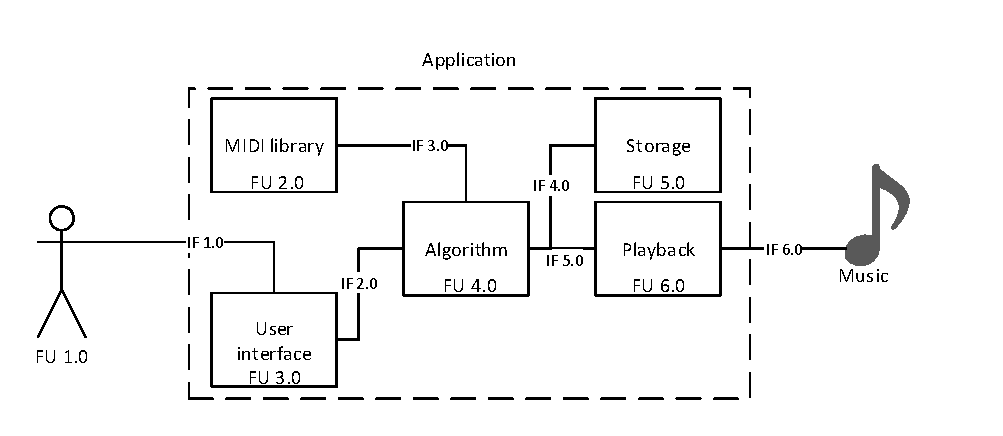
\includegraphics[width=400px]{../images/architecture.pdf}}
\caption{Functional architecture}
\label{ims:funcarch}
\end{figure}

By incorporating all these elements we can concretely describe the project in discrete components in a functional architecture diagram, see figure \ref{ims:funcarch}.

\section{Functional architecture}
\subsection{Functional Unit 1 - Operator}
The operator is responsible for interacting with the application. The operator will select the style or category for composition and instruct to application to compose music.
If a certain piece of music is to be save the operator will be responsible for instructing the application to do so and to select the location the \ac{MIDI} file is to be saved

\subsection{Functional Unit 2 - MIDI library }
The MIDI library is a large collection of \ac{MIDI} files. The files in the \ac{MIDI} library are organized into categories. Each category represents a certain style of music
The algorithm will utilize a subset of the library (a category) as input.

\subsection{Functional Unit 3 - User Interface}
The user interface is the front end of the application. The operator interacts with this functional unit in order to instruct the application what to do.

The user interface should be designed in a user-friendly manner in order to accommodate the operator.
A conceptual user interface is shown in figure \ref{ims:conceptuserinterface}. 

This user interface allows the user to select a certain style, instruct the algorithm to compose music and to save or play back a piece of music once it is composed.

\subsection{Functional Unit 4 - Algorithm}
The algorithm is the central part of this project. The algorithm converts the input \acp{MIDI} into output \ac{MIDI}.

The algorithm will utilize a category of \ac{MIDI} files from the \ac{MIDI} library in order to compose a new piece of music not in the \ac{MIDI} library.

The output piece of music will represent the style of music that was used as input.
The possible types of algorithms were discussed in section \label{chap:comp_algo}

\subsection{Functional Unit 5 - Storage}
This unit is responsible for storing the output \ac{MIDI} from the algorithm into a \ac{MIDI} file.

\subsection{Functional Unit 6 - Playback}
This unit is responsible for playing back the output \ac{MIDI} from the algorithm through an audio output device

\section{Interfaces}
The interfaces indicate the interaction between different functional units.
The interfaces have the following functions:
\\Interface:
\begin{enumerate}
\item Interface between the user and the user interface. This input would be from a input peripheral device.
\item Interface between the user interface and the algorithm. The interface calls the algorithm with the parameters supplied by the user such as when to start and what type of style was selected
\item Interface between the \ac{MIDI} library and the algorithm. The input to the algorithm is a selection of \acp{MIDI}. The interface converts \ac{MIDI} files into a format required by the algorithm
\item Interface between the algorithm and storage. This interface converts the output from the algorithm into the \ac{MIDI} file format
\item Interface between the algorithm and playback. This interface converts the output from the algorithm into a format that is ready for playback through the playback functional unit.
\item Interface between the playback and the music. This represents the audio output device and it's workings.
\end{enumerate}

\chapter{Operational Flow}

The operational flow indicates the interaction between the operator and the application and how the operator should use it.

\begin{figure}[ht]
\centerline{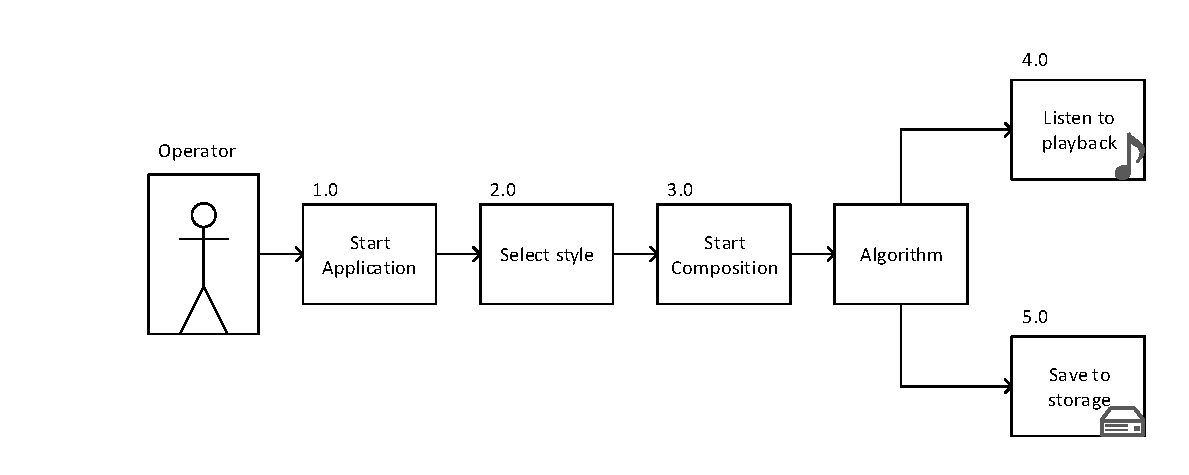
\includegraphics[width=400px]{../images/operational_flow.pdf}}
\caption{Operational Flow}
\label{ims:oppflow}
\end{figure}

\begin{figure}[ht]
\centerline{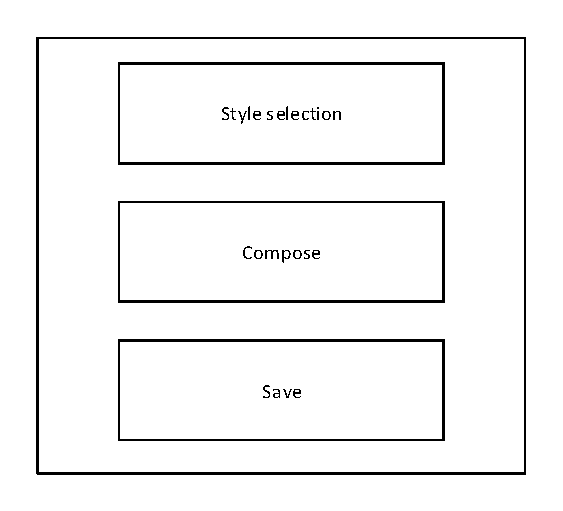
\includegraphics[width=150px]{../images/user_interface.pdf}}
\caption{Conceptual user interface}
\label{ims:conceptuserinterface}
\end{figure}

Figure \ref{ims:oppflow} shows how the operator interacts with the application. Figure \ref{ims:conceptuserinterface} shows a conceptual user interface with which the operator would interact.

For this application, the operator selects the style of music to be composed; instructs the application to compose the music according to the selected style and then to instruct the application to either play back the piece of generated music or save it to storage.

\begin{figure}
\centerline{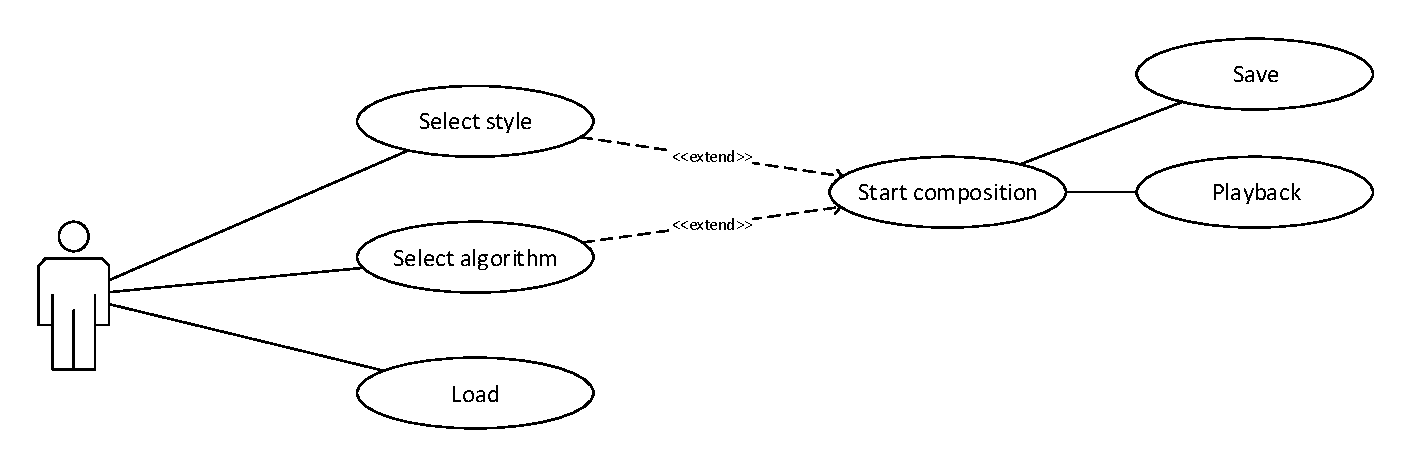
\includegraphics[width=350px]{../images/op_use_case.pdf}}
\caption{Application interaction use case}
\label{ims:opusecase}
\end{figure}

Figure \ref{ims:opusecase} shows a more in-depth interaction between the user and the application. 
The application allows the user to:
\begin{enumerate}
\item Select the style for composition
\item Select the algorithm to be used for composition
\item Load a previously generated melody
\item Save a generated melody
\end{enumerate}

Some considerations need to be taken to ensure that the interface to the application is as user-friendly as possible. 

\begin{enumerate}
\item The design of the interface should be clean and minimilistic. 
\item Clear instructions should be given to the user when there is a possibility of ambiguity.
\item Images and icons should be used as visual aids for buttons or to indicate the function of a feature
\item Seperate functional features should be seperated in the interface. The following areas should have seperate section in the interface
	\begin{itemize}
	\item Playback, saving and loading
	\item Generation of melodies
	\item Optional options and parameters for algorithms
	\end{itemize} 
\end{enumerate}

Functionally, it makes sense for the user to choose the filename and path of the melody to be saved. Similarly the user should be able to select which previously generated melody should be loaded.

\chapter{Conclusion}
In order to solve the problem of generating music algorithmically the task was broken down into its functional architecture. From this each functional unit and its interaction is made apparent. The core component of this project is the algorithm which is used to compose music
\part{Algorithms} \label{part:algo}
%!TEX root = ../Report.tex
%************************************************

% Algorithms

\chapter{Introduction}
In this part possible algorithms will be investigated, designed for composition and implemented in order to determine which are viable for inclusion into the application.

The system operates on MIDI files. MIDI events are processed and the resulting notes are stored in a sequence where the pitch and duration of each note are recorded. A note is represented in MIDI as a number from $0$ to $127$.
Thus for each MIDI track a monophonic melody can be extracted.

A large set of MIDI files (~600) were collected for style of music. The following categories were used to test the algorithms:
\begin{enumerate}
\item A mixture of Classical music (665)
\item A mixture of retro video game music (395)
\item A mixture of Pop and Top40 (1370)
\item A mixture of Classic Rock (2274)
\item A mixture of Jazz music (114)
\item A mixture of Dance and Techno (214)
\end{enumerate}

These categories are not the final list of styles that will be included into the end user application.


\chapter{Representation}
This section discusses how music is represented internally in the system and how the data structures are designed. 
Proper data structures are extremely important for good algorithms \footnote{Bad programmers worry about the code. Good programmers worry about data structures and their relationships \mytilde Linus Torvalds}.

\section{Assumptions and simplifications}
For this system our model of music is simplified and we do not make provisions for chords. Melodies are monophonic and are simply a list of notes of their durations.

Furthermore, we assume all files are \ac{MIDI} \emph{Track type $1$}.

\section{Note}
A note is the most basic element. A note consists of:
\begin{enumerate}
\item Note duration - A whole note, half note, quarter note and so on.
\item Note pitch - A number representing the note pitch, in MIDI scale. $0 \leq P < 128, p \in \mathbb{Z}$
\end{enumerate}

From these properties the following can be derived:
\begin{enumerate}
\item Octave - Every twelve note pitches represent one octave
\item Chromatic tone - An integer from 0 to 11. Also corresponds to the name of the note for example C, C\#, G, A\#
\end{enumerate}
These properties are related to the Note pitch by:
\[P = 12o + p \]
where $o$ is the octave and $p$ is the chromatic tone

\section{Melody sequence}
A melody sequence is simply a list or sequence of notes:
\[\{N_1, N_2, \ldots, N_n\} \]
Where $N$ is a note.

Most algorithms operate only on the melody sequence and output a melody sequence. Some algorithms may optionally require information on the instrument in which the melody sequence is played.

\section{Track}
A track contains a sequence of melody sequences and is also described by an instrument in which the sequence are played.

\section{Composition}
A composition is a sequence of tracks which can be played in parallel. 
MIDI files are converted into compositions.

\begin{figure}
\centerline{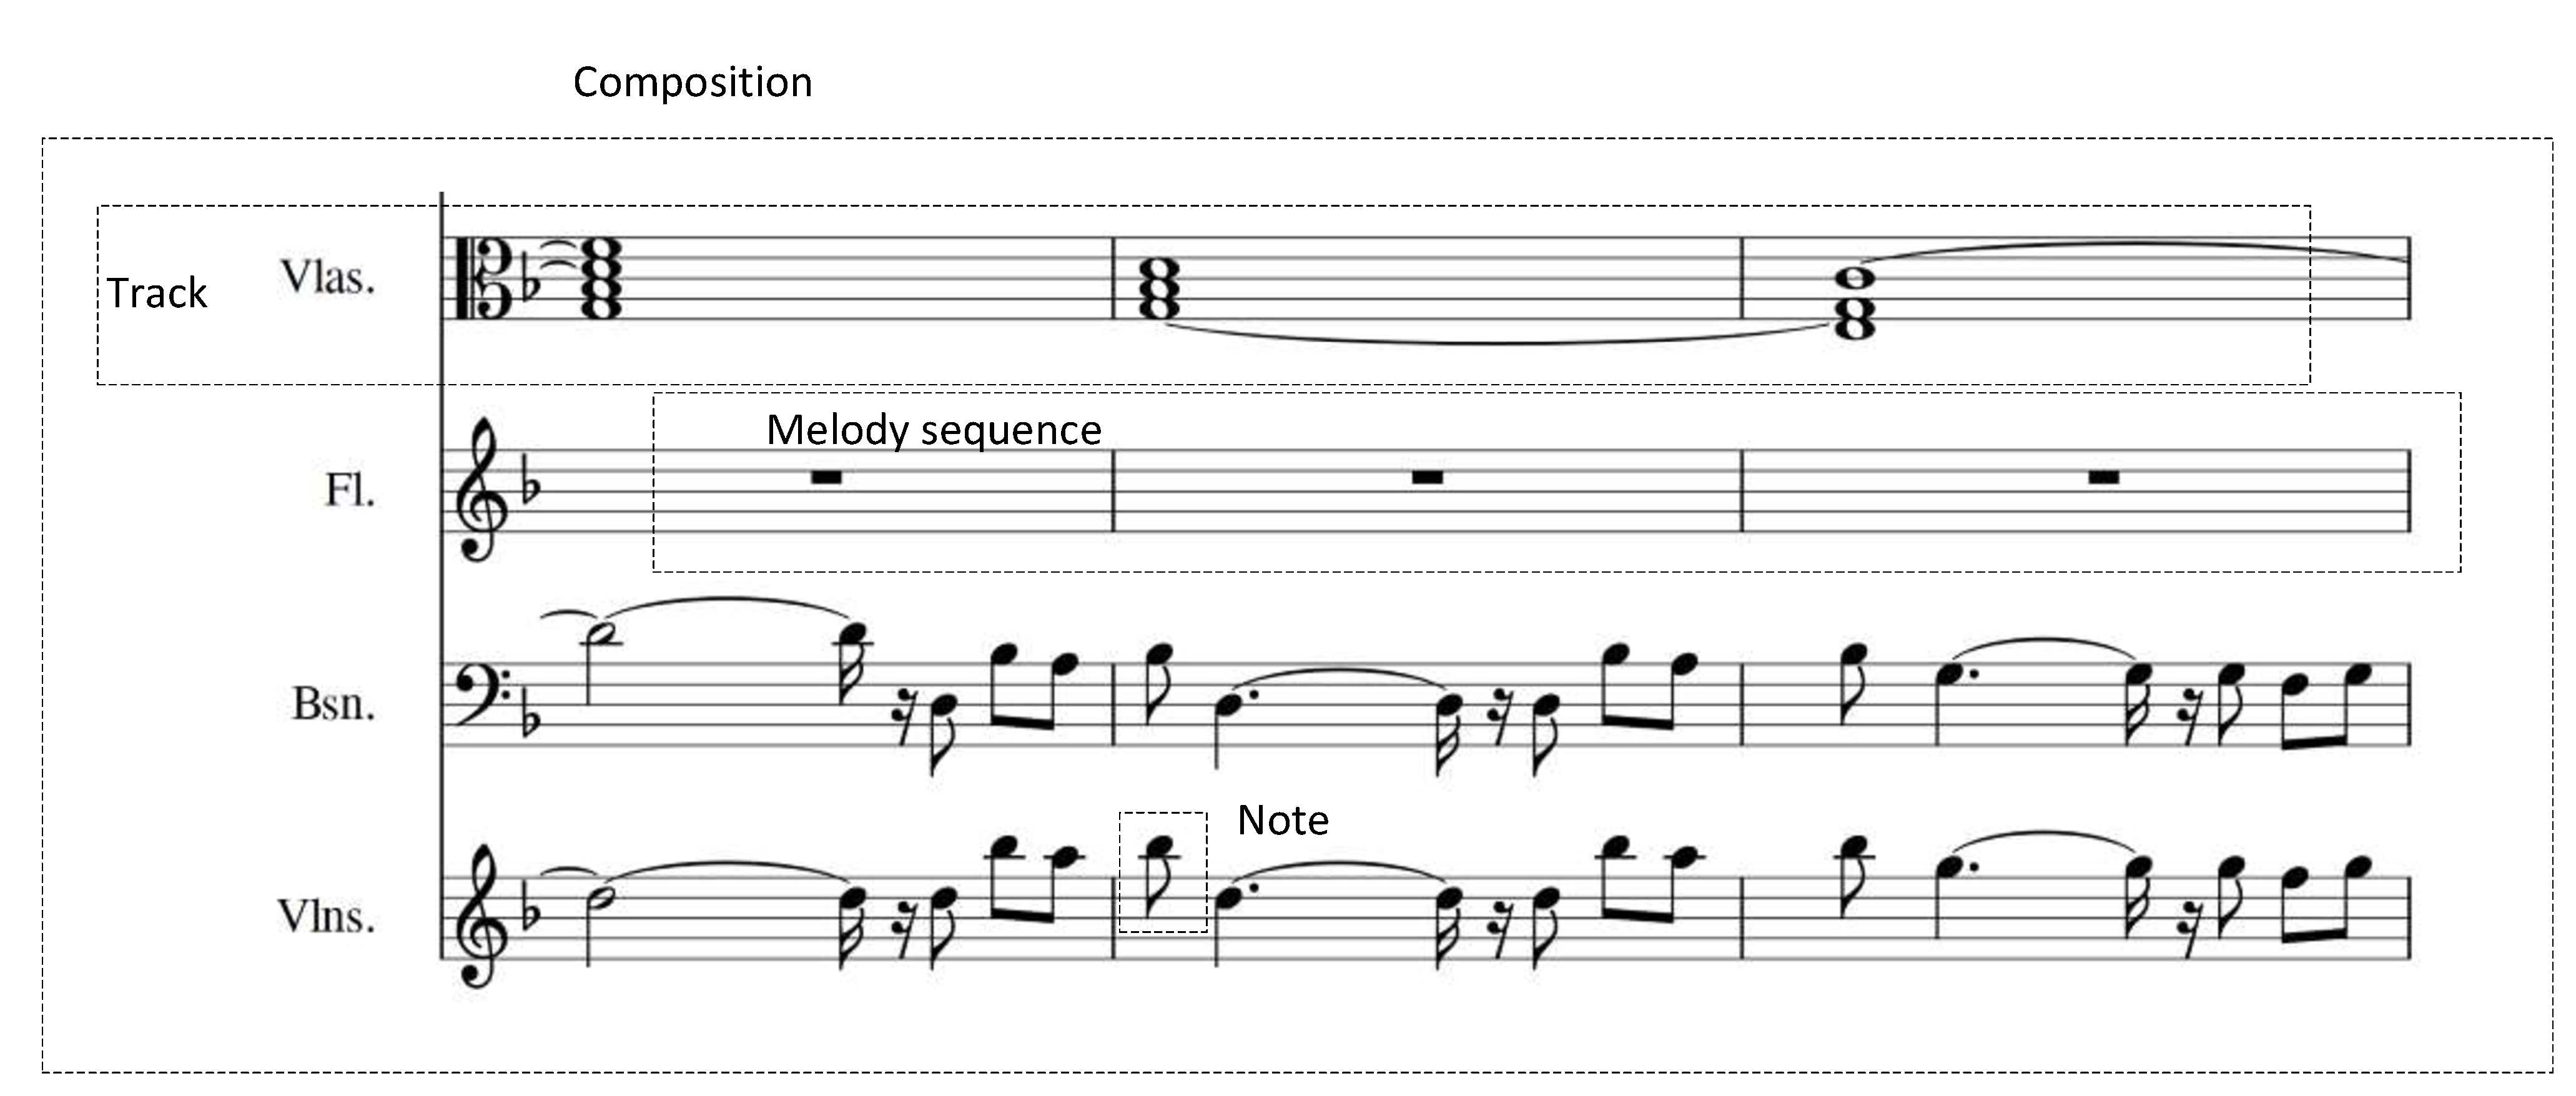
\includegraphics[width=400px]{../images/composition_illustration.pdf}}
\caption{Illustration of a composition and its elements}
\label{ims:compillu}
\end{figure}

Figure \ref{ims:compillu} illustrates the relation between the above mentioned structures for a midi file.

\begin{figure}
\centerline{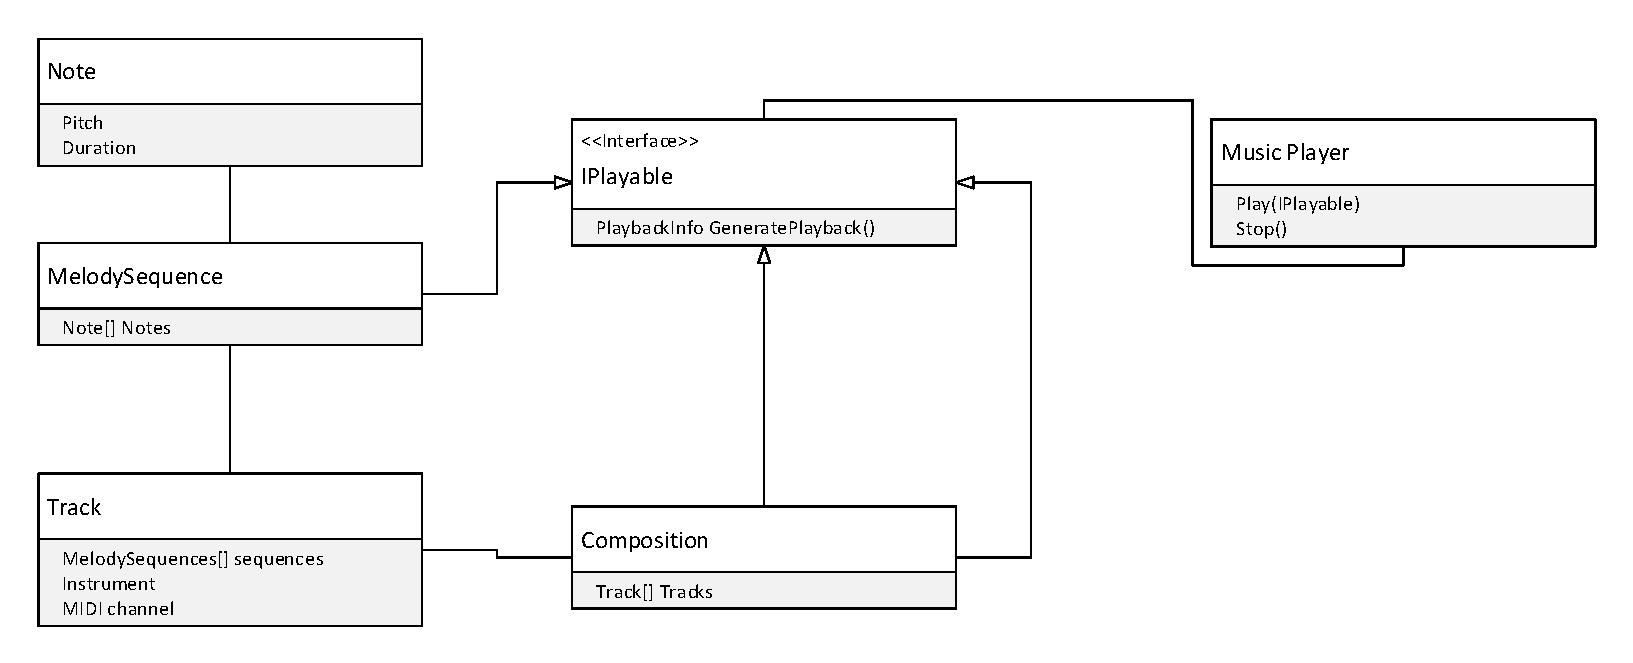
\includegraphics[width=400px]{../images/uml_notes.pdf}}
\caption{UML diagram indicating the interaction between compositional elements}
\label{ims:uml_notes}
\end{figure}

Figure \ref{ims:uml_notes} indicates the interactions between Notes, Melody Sequences, Tracks, Compositions and the Music Player.

\section{Generator Algorithms}
%In this section the data structures are discussed which aid with the generating of melody sequences through the algorithms that are discussed in this section. 
All algorithms considered in this section derive from the interface INoteGenerator. This exposes basic functionality for generating a algorithm and determining whether the Next function can be called. The Next function returns a new random melody sequence without resetting the generator. See figure \ref{ims:uml_generator}.

Using this abstracted design allows the user to select any algorithm to be used for composition, and the main application logic only needs to call Generate() or Next() as required. The details of the algorithm implementation is abstracted away.

\begin{figure}
\centerline{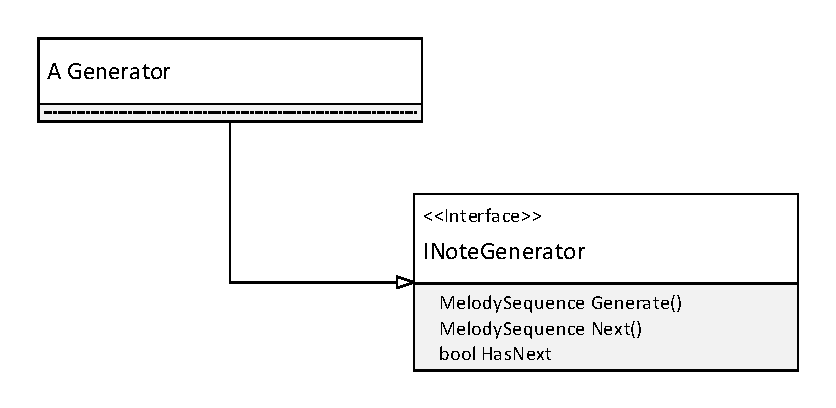
\includegraphics[width=250px]{../images/uml_generator.pdf}}
\caption{UML diagram of a generator class}
\label{ims:uml_generator}
\end{figure}

%%% START GENETIC %%%%%%%%%%%%%%%%%%%%%%%%%%%%%%%%%%%%%%%%%%%%%%%%%%%%%%%%%%%%%%%%%%%%%%%%%%%%%%%%%%%%%%%%%%%%%%%%%%%%%%%%%

%%%%%%%%%%%%%%%%%%%%%%%%%%%%%%%%%%%%%%%%%%%%%%%%%%%%%%%%%%%%%%%%%%%%%%%%%%%%%%%%%%%%%%%%%%%%%%%%%%%%%%%%%%%%%%%%%%%%%%%%%


\chapter{Genetic Algorithm for Melody Generation}

For this project a quantitative approach is taken toward algorithmic music composition. In particular quantitative metrics will be used in the fitness functions of the genetic algorithm.

In section \label{chap:comp_algo} the following types of music composition algorithms were investigated:
\begin{enumerate}
\item Neural Networks
\item Genetic Algorithms
\end{enumerate}
In the literature review, it was found that the pieces generated by neural networks lack musical coherency and perform poorly as the length of music increases. Some other attempts have met slightly more success although the overarching view for neural networks in music composition seems grim\footnote{Although neural networks as functions in genetic algorithms have had better success}.

Genetic algorithms are viable for algorithmic composition for the following reasons:
\begin{enumerate}
\item They allow for great flexibility in implementation and music representation
\item There has been some research into possible fitness functions for evolutionary music composition.
\item Great amount of variety made possible by different fitness functions and by the representation of music used in \acp{GA}
\end{enumerate}

In section \ref{sec:chapfitness} the following fitness functions were covered:
\begin{enumerate}
\item Zipf's law
\item Cosine similarity
\item Neural Networks
\item Normalized Compression Distance
\item Interactive evaluation\footnote{An interactive fitness function imposes a bottleneck on the performance of the system}
\end{enumerate}

\begin{figure}
\centerline{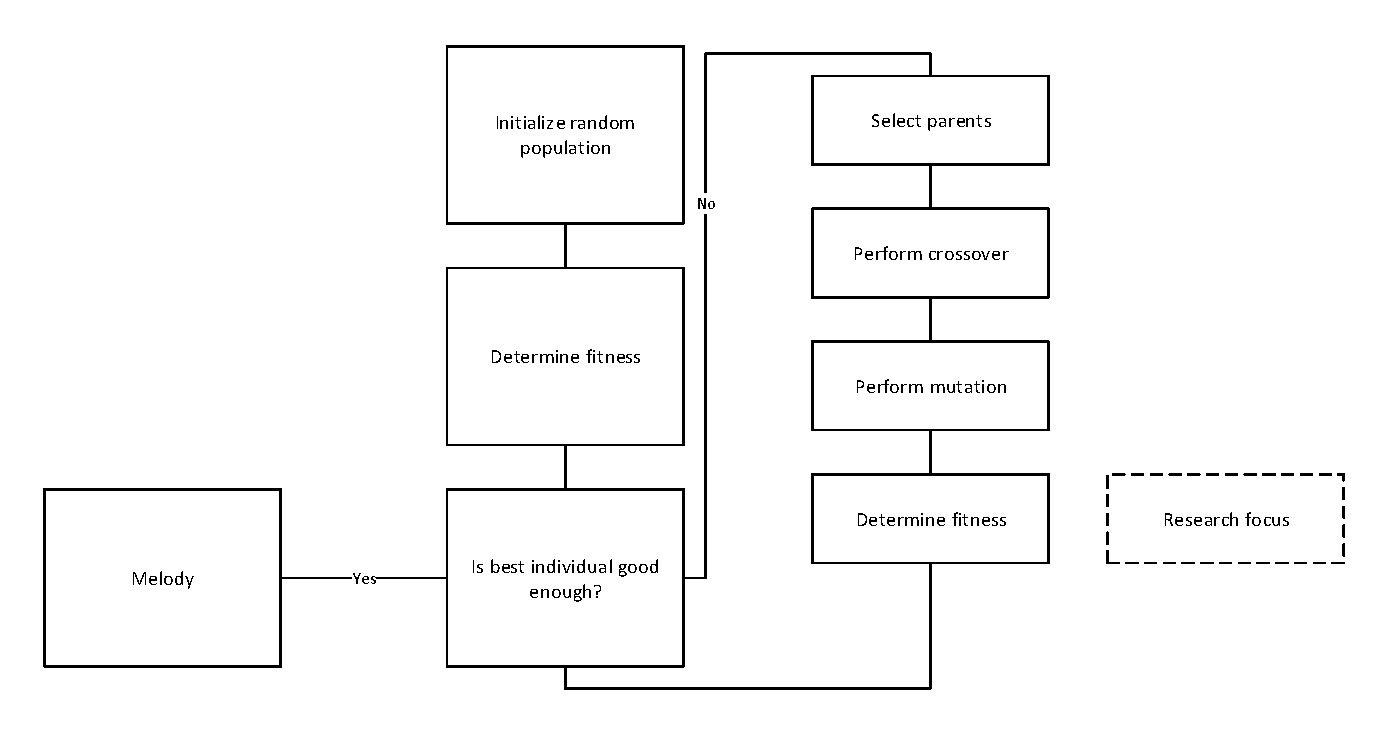
\includegraphics[width=400px]{../images/GA_flow.pdf}}
\caption{Flow diagram of the operation of a genetic algorithm}
\label{ims:geneticflow}
\end{figure}

Figure \ref{ims:geneticflow} indicates the flow for a genetic algorithm/program.

\section{Introduction}

Evolutionary algorithms come in a variety of different types. The two most common types found are Genetic Algorithms and Genetic Programming. Genetic Programming has been found to be more suitable for composing music than genetic programming due to music forming a hierarchical structure.

A flexible genetic programming model will be developed that is able to function with the investigated fitness functions. 

The two largest problems for a evolutionary computing problem is:
\begin{enumerate}
\item Obtaining a good representation of the problem
\item Obtaining a good fitness function
\end{enumerate}
A genetic algorithm modifies the structure of an individual, if the structure is poorly chosen then a optimal solution wont by found by the algorithm.
An ideal fitness function is able to quantify the fitness of an individual. An ideal fitness function in music composition would map the human perception of pleasantness into a fitness value. 

\section{Fitness functions}
The fitness function is a primary research interest in genetic music composition. 
An ideal fitness function captures the human perception of pleasantness in music, however there have not been practical advances in this direction. Statistical measures will rather be used.

Of the set of investigated fitness functions only the following functions will be implemented:
\begin{enumerate}
\item Cosine similarity
\item Normalized Compressions Distance
\end{enumerate}
Since interactive evaluation is slow, Zipf's law is superseded by Cosine similarity and training neural networks as fitness functions pose a large number of problems.

\section{Music Representation}
A flexible music representation can also be developed for the Genetic Programming algorithm. 

\begin{figure}
\center
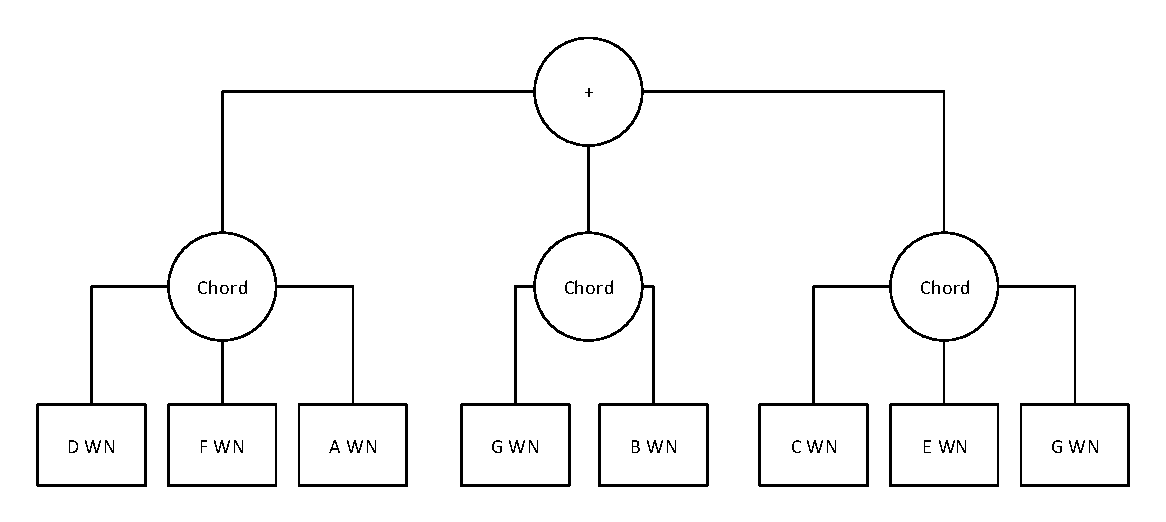
\includegraphics[width=350px]{../images/tree_stuct_piece.pdf}
\caption{A music piece in a tree structure}
\label{ims:musicpieceextrree}
\end{figure}
%Where the :=: operator indicates pieces are played in parallel (chords) and :+: indicates pieces are played in series. a,b,d,e,f,g indicate the note pitch and wn indicates a whole note.
Figure \ref{ims:musicpieceextrree} indicates a polyphonic melody in tree form. Strictly a chord is a set of three or more notes that are played simultaneously. Note that the second branch is only constituted of two notes.
\\
\\
Minsky and Laske \cite{Minsky1992} argued for a tree representation of music since the tree represents the hierarchical nature of music. The tree representation is much more complex than data structures such as vectors that are used in \acp{GA}.

Some authors \cite{Biles1994} limit the search space by ensuring that melodies are in a certain scale.
\\
\\
The representation will model \ac{MIDI} events and manipulation of them. A simpler tree structure will be developed as chords will not be supported by the system. The operators of the tree will be given in the next section.

\section{Genetic operators}
Several different operators can be performed on the tree structure. In figure \ref{ims:musicpieceextrree} the serial concatenation and parallel concatenation operators were shown.
Some additional operators which may be employed include:
\begin{itemize}
\item Repetition - Repeating a segment a given number of times
\item Shift note pitches - Shift all pitches of notes by a certain amount
\item Duration elongation or contraction - For example a slow operation doubles the duration
\item Transposition - Moving note positions relatively
\item Retrograde - Reversed order of notes
\end{itemize}

Genetic operations such as mutation and crossover may be used conventionally.

\section{Metrics} \label{chap:metrics}
Feature extraction is required to reduce the search space and to provide the fitness function with musically meaningful measures with which to rate the fitness. In this section we cover some quantitative metrics that may be used as measures to identify or represent music.

The frequencies of a metric is used in the Cosine Similarity fitness function.

The different types of metrics that will be used include:
\begin{enumerate}
\item Pitch - List of pitches
\item Pitch differences - Store first pitch, thereafter list consecutive pitch differences
\item Chromatic tone - 12 pitch class. Notes are reorganized into 12 classes.
\item Note durations - durations of notes
\item Pitch distance - intervals between repetition of pitches
\item Chromatic tone distance - intervals between repetition of chromatic tones  
\item Melodic interval - intervals between the current note and the previous note
\item Melodic bi-gram - Pairs of melodic intervals
\item Rhythm - duration of a note in addition to the following rest
\item Rhythmic interval - relationship between adjacent note rhythms
\item Rhythmic bi-gram - Pairs of adjacent rhythmic intervals.
\item Chromatic tone duration - A pair of the chromatic tone and the duration
\end{enumerate}

Let $p$ denote the pitch of the note, where $0 \leq p < 128$.
Then the chromatic tone is given by:
\[c = p \% 12\]
where $\%$ indicates the modulo operation.
The melodic interval is given by:
\[\text{mi}_k = p_k - p_{k-1} \]
The melodic bi-gram is given by:
\[b_k = (\text{mi}_k, \text{mi}_{k+1}) \]
Let $r$ indicate the note duration with rests
Then the rhythmic interval is given by:
\[\text{}ri_k = \frac{r_k}{r_{k-1}} \]
and the rhythmic bi-gram
\[\text{rk}_k = (\text{ri}_k, \text{ri}_r) \]

In this manner we can build a metric vector, let $m_i(A)$ denote a metric's value at position $i$ for musical piece $A$. Then the metric vector is given by $\vec{M}_A = \{m_0(A), m_1(A), \ldots, m_n(A) \}$ 


\section{Fitness functions}

In this section two fitness functions are described which can be used for the Genetic Algorithm. \ac{NCD} and Cosine Similarity are described here.

The fitness functions described in this section require the phenotype of an individual. Thus it is necessary to parse the genotype, the genetic tree of the individual down into a sequence of notes.

\subsection{Cosine similarity}
Some fitness functions such as Cosine similarity and Zipf's law operate on the features of music. 

Cosine similarity can be applied to the metrics listed in section \ref{chap:metrics}. Let $\vec{a_m}$ denote the vector of metric values according to a metric $m$ for a music piece $A$ and $\vec{b_m}$ denote the vector by $m$ for a music piece $B$ then the similarity between $A$ and $B$ is given by:
\[\text{similarity}_m(A,B) = \frac{\vec{a_m} \cdot \vec{b_m}}{|\vec{a_m}| |\vec{b_m}|}\]

A set of metrics may be used. 
The fitness function is then given by a weighted average:
\[f = \frac{1}{N} \sum_{k}^N w_k \times \text{similarity}_{mk}(A,B) \]
where $w$ is a weight assigned to metric $mk$.

\subsection{Normalized compression distance}
In order to utilize \ac{NCD} both pieces being tested need to be encoded in the same way. Musical pieces may be encoded as metric vectors as listed in section \ref{chap:metrics}. More complex metrics may be utilized however there has been no thorough investigation into this.

The \ac{NCD} as an estimate to the \ac{NID} was covered in section \ref{sec:class_ncd}.

In order to utilize the \ac{NCD} as a fitness function the following steps are taken:
\begin{enumerate}
\item Encode a set from the \ac{MIDI} library according to a metric. Let $\Omega = \{\vec{M_0}, \vec{M_1}, \ldots, \vec{M_n}\}$ for musical pieces $0$ to $n$ in the \ac{MIDI} library that accord to a certain style.
\item Encode the population individual $x$ according to the metric (Given by $\vec{M_x}$).
\item Employ the fitness function
\end{enumerate}

The fitness function that will be used is:
\[f(x) =  \left(\sum_{\vec{T}\in\Omega} \text{NCD}(\vec{M_x}, \vec{T}) \right)^{-1}\]

The following representation scheme was designed:
\begin{itemize}
\item A note is surrounded in parentheses.
\item The note pitch is given by the chromatic tone symbol followed the the octave number.
\item The duration is given after a hyphen. A standard note duration is used where possible otherwise the numeric value is given.
\item 
A sequence of notes can be given by: 
	\begin{lstlisting} 
	(C4-wn)(C3-qn)(C5-qn) 
	\end{lstlisting}
\item When tracks are played the symbol || is used to denote notes playing in parallel.
\item A instrument can optionally be specified at the start.
\end{itemize}

For example:
\begin{lstlisting}
(Trombone (C6-3)(C5-tn)(G5-tn)(C6-3)(E5-tn)(G5-tn)(G6-3)(C5-tn)(G5-tn)(G6-en)(E5-tn)(G5-tn)(A6-3)(F4-tn)(F5-tn)(C5-tn)(A6-en)(F5-tn)(G4-tn)(G6-qn)...
\end{lstlisting}


\section{Methodology}
%TODO
In this section the setup and parameters of the experiment to produce melodies with Genetic Algorithms are outlined.

In order to compose a melody with a genetic algorithm a fitness function is required to rate the fitness of an individual. The following fitness functions were investigated:
\begin{enumerate}
\item \ac{NCD}
\item Cosine similarity
\end{enumerate}

A proper representation is required. A melody is represented in tree form. The tree is given a maximum depth of $(\log_2 x) +  3$ where $x$ is the average number of notes in a melody.

The following genetic operators were used:
\begin{enumerate}
\item Concatenation - The addition of two nodes
\item Duration Shift - Scale the duration with a factor
\item Pitch Shift - Move all note pitches a certain number up or down
\item Repeat - Repeat a note a certain number of times
\item Swap - Swap the positions of two notes
\end{enumerate}

The following metrics were investigated:
The different types of metrics that will be used include:
\begin{enumerate}
\item Pitch differences
\item Chromatic tone duration 
\item Chromatic tone distance 
\item Pitch distance
\item Melodic interval
\item Melodic bi-gram
\item Rhythmic interval 
\item Rhythmic bi-gram
\end{enumerate}

The duration and pitch a note may take on is limited to the available note pitches and durations in the dataset.

The parameters of the Genetic Algorithm were set as follows:
\begin{itemize}
\item Chromosome representation - Tree form
\item Mutation rate - 0.1
\item Crossover rate - 0.9
\item Population - 30
\item Selection - Elite selection
\item Auto shuffling of individuals in population after every epoch
\item Standard amount of generations - 1000
\end{itemize}

The individual with the highest fitness was used as the resulting chromosome. 
Since the result is in tree form it needs to be parsed into a simple sequence of notes.

\section{Results}


A simple test was done comparing the \ac{NCD} and Cosine Similarity fitness functions against each other. The Cosine Similarity was tested using the Chromatic Time Duration, Rhythmic Bigram and Melodic Bigram frequency metrics. The average fitness and maximum fitness were compared against each other. The genetic algorithm was run for $100$ epochs.

% Table generated by Excel2LaTeX from sheet 'Sheet3'
\begin{table}[htbp]
  \centering
  \caption{Comparison of Fitness Functions}
    \begin{tabular}{l|rr}
    \toprule
          & Performance &  \\
    \midrule
          & Average Fitness & Maximum Fitness \\
    NCD   & 0.0016 & 0.00156 \\
    Metric Similarity & 0.666 & 0.683 \\
    \bottomrule
    \end{tabular}%
  \label{tab:ffcompare}%
\end{table}%

Table \ref{tab:ffcompare} shows the results. It can be seen that the maximum fitness achieved by the \ac{NCD} fitness function in 100 epochs is only $0.0016$ whereas the MetricSimilarity is at $0.683$. The pleasantness of the produced melody by \ac{NCD} is also worse, however this may be due to the lower fitness.
However generation time is important for the Genetic Algorithm and the \ac{NCD} fitness function is slow.


% Table generated by Excel2LaTeX from sheet 'Sheet3'
\begin{table}[htbp]
  \centering
  \caption{Performance comparison between frequency metrics}
    \begin{tabular}{l|llll}
    \toprule
          & MaxFit & AvgFit & Time(ms) & Pleasantness \\
    \midrule
    Chromatic Tone & 0.944 & 0.9439 & 8992  & 4 \\
    Chromatic Tone Distance & 0.98  & 0.98  & 11017 & 5 \\
    Chromatic Tone Duration & 0.936 & 0.935 & 13688 & 5 \\
    Melodic Bigram & 0.857 & 0.857 & 3900  & 5 \\
    Melodic Interval & 0.985 & 0.985 & 9037  & 5 \\
    Pitch & 0.832 & 0.832 & 14001 & 4 \\
    Pitch Distance & -     & -     & -     & - \\
    Rhythm & 0.952 & 0.952 & 367   & 4 \\
    Rhythmic Bigram & 0.995 & 0.995 & 4729  & 7 \\
    Rhythmic Interval & 0.996 & 0.996 & 5501  & 6 \\
    \bottomrule
    \end{tabular}%
  \label{tab:metriccomp}%
\end{table}%

The maximum fitness, average fitness, time (given in milliseconds) and subjective pleasantness were evaluated for each frequency metric. See table \ref{tab:metriccomp}. 

In order to construct a target piece for the metric similarity the notes of the first track of each midi file were sequenced. The total notes were $662923$. Note that some metrics have larger time than others, this is due to the amount of features or categories for that metric and does not necessarily indicate that metric is slow. The pitch distance metric was excluded as it took too long.

From table \ref{tab:metriccomp} it can be seen that subjectively rhythm is important.




\begin{figure}
\centerline{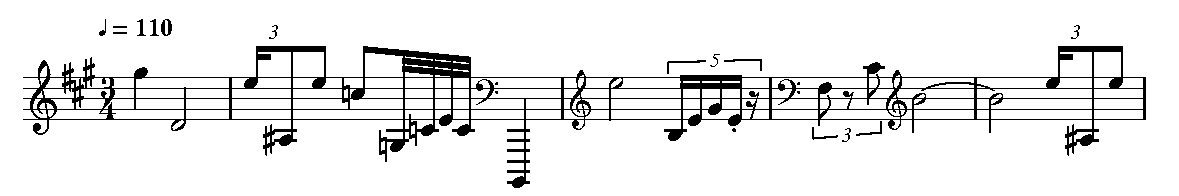
\includegraphics[width=300px]{../images/genetic_ncd.pdf}}
\caption{Melody produced with a Genetic Algorithm using the \ac{NCD} fitness function}
\label{ims:genetic_mel_ncd}
\end{figure}

\begin{figure}
\centerline{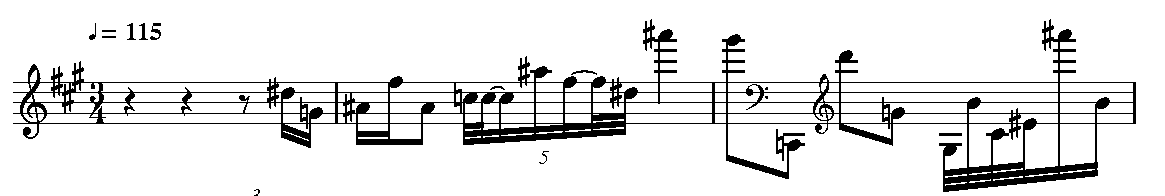
\includegraphics[width=300px]{../images/genetic_cosine_ctd_rb.pdf}}
\caption{Melody produced with a Genetic Algorithm using the cosine similarity fitness function with chromatic tone duration and rhythmic bigram metrics}
\label{ims:genetic_mel_ctdrb}
\end{figure}

\begin{figure}
\centerline{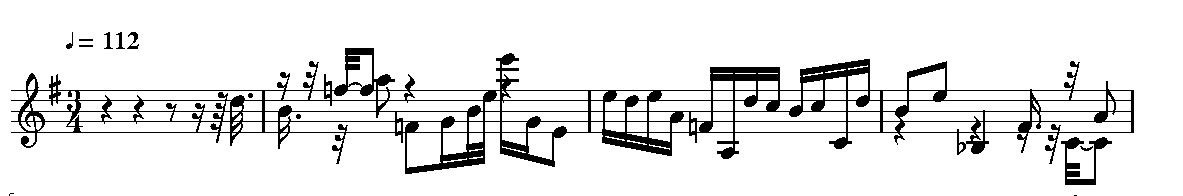
\includegraphics[width=300px]{../images/genetic_cosine_all.pdf}}
\caption{Melody produced with a Genetic Algorithm using the cosine similarity fitness function with all frequency metrics}
\label{ims:genetic_mel_mall}
\end{figure}

Figure \ref{ims:genetic_mel_ncd} indicates an excerpt of a melody produced with the Genetic Algorithm using the \ac{NCD} fitness function. The \ac{NCD} fitness function produced the worst results. The resulting melodies sound chaotic and random. \ac{NCD} is also slow, as each individual needs to be converted to its text representation and then be compressed in order to obtain its compressed distance.

The melody produced in figure \ref{ims:genetic_mel_ctdrb} using the cosine similarity fitness function was rather pleasant and the rhythmic bigram and chromatic tone duration -frequency metrics produce pleasant melodies.

The melody produced in figure \ref{ims:genetic_mel_mall} used the cosine similarity fitness function using all the frequency metrics. At times the melody is pleasant however off-sounding or out of key notes are a common occurrence. The melodies also don't have structure. This indicates that some of the frequency metrics either don't work well in conjunction with each other or some frequency metrics have a negative effect on the pleasantness of melodies. 

The following frequency metrics produced good or pleasant results:
\begin{enumerate}
\item Chromatic tone distance - intervals between repetition of chromatic tones
\item Melodic interval - intervals between the current note and the previous note
\item Rhythmic bigram - Pairs of adjacent rhythmic intervals
\item Chromatic tone duration - A pair of the chromatic tone and the duration
\end{enumerate}


\section{Conclusion}

The decision was made to utilize a genetic programming algorithm since the tree structure accommodates the hierarchical nature of music. Genetic programming provides flexibility, variety of possible styles and a large amount of research has been done one fitness functions for genetic algorithms.

Fitness functions require good measures that make it possible to rate musical pieces quantitatively. A set of metrics were developed in which musical pieces can be measured.

Two fitness functions, namely Cosine similarity and \ac{NCD} were developed to incorporate these metrics.

The results of different fitness functions were compared. \ac{NCD} performed the worst. Not all of the frequency metrics required for the cosine similarity fitness function produced good results. A subset of good frequency metrics were explored.


%%% END GENETIC %%%%%%%%%%%%%%%%%%%%%%%%%%%%%%%%%%%%%%%%%%%%%%%%%%%%%%%%%%%%%%%%%%%%%%%%%%%%%%%%%%%%%%%%%%%%%%%%%%%%%%%%%

%%%%%%%%%%%%%%%%%%%%%%%%%%%%%%%%%%%%%%%%%%%%%%%%%%%%%%%%%%%%%%%%%%%%%%%%%%%%%%%%%%%%%%%%%%%%%%%%%%%%%%%%%%%%%%%%%%%%%%%%%


\chapter{Melody generation with a Hidden Markov Model}
\section{Introduction}
An attempt was made to use a hidden Markov model to generate melody sequences.

A \ac{HMM} is a statistical Markov model where the assumption is made that the system being modeled  is a Markov process with hidden states. See section \ref{sec:hmm_backround} for more information on Hidden Markov Models for melody generation.

\section{Methodology}
In order to train the \ac{HMM}, that is to re-estimate the \ac{HMM} parameters the unsupervised algorithm of Baum-Welch was used. The update rules are given in section \ref{sec:hmm_backround}. However the regular update rules of Baum-Welch only cover an update for a single observation.

In order to operate on multiple observations the independence assumption was made, that is:
\[ P(\emph{O} | \lambda) = \prod_{k=1}^K P(O^{(k)} | \lambda) \]
For which the update rules according to Levinson are:
\begin{enumerate}
\item State transition:
\[ a'_{mn} = \frac{\sum^K_{k=1} \sum^{T_k -1 }_{t=1} \xi^{(k)}_t (m,n)}{\sum^K_{k=1} \sum^{T_k-1}_{t=1} \gamma_t^{(k)}(m)} \]

\item Observation emission:
\[ b'_n (m) = \frac{\sum^K_{k=1} \sum^{T_k -1 }_{t=1, o_t^{(k)} = v_m} \gamma^{(k)}_t (n)}{\sum^K_{k=1} \sum^{T_k-1}_{t=1} \gamma_t^{(k)}(n)} \]

\item Initial state:
\[ \pi'_n = \frac{1}{K} \sum^K_{k=1} \gamma_1^{(k)}(n)  \]

\end{enumerate}

Special care was taken to to avoid underflows. All probabilities were stored as log probabilities.


For this experiment a simple first order \ac{HMM} is constructed with a ergodic structure. In addition the following constraints were made:
\begin{itemize}
\item The amount of states of the \ac{HMM} was constrained to $100$
\item The duration of all notes were restricted to be in \{tn, sn, en, qn, hn, wn \} where wn is a whole note, qn is a quarter note and so on. 
\end{itemize}

All uniques notes were linked with a unique integer id with the use of a dictionary. 

In order to test the model it was trained on datasets of different styles. No distinction was made between different instruments as was the case with the Markov Chain experiment.
The melody sequences of each composition was used as the input data for the modified Baum-Welch training algorithm. The number of iterations was set to $100$.


\section{Results}
Since the model is of first order it produces melodies without overall structure. This is to be expected.

\begin{figure}[h!]
\centerline{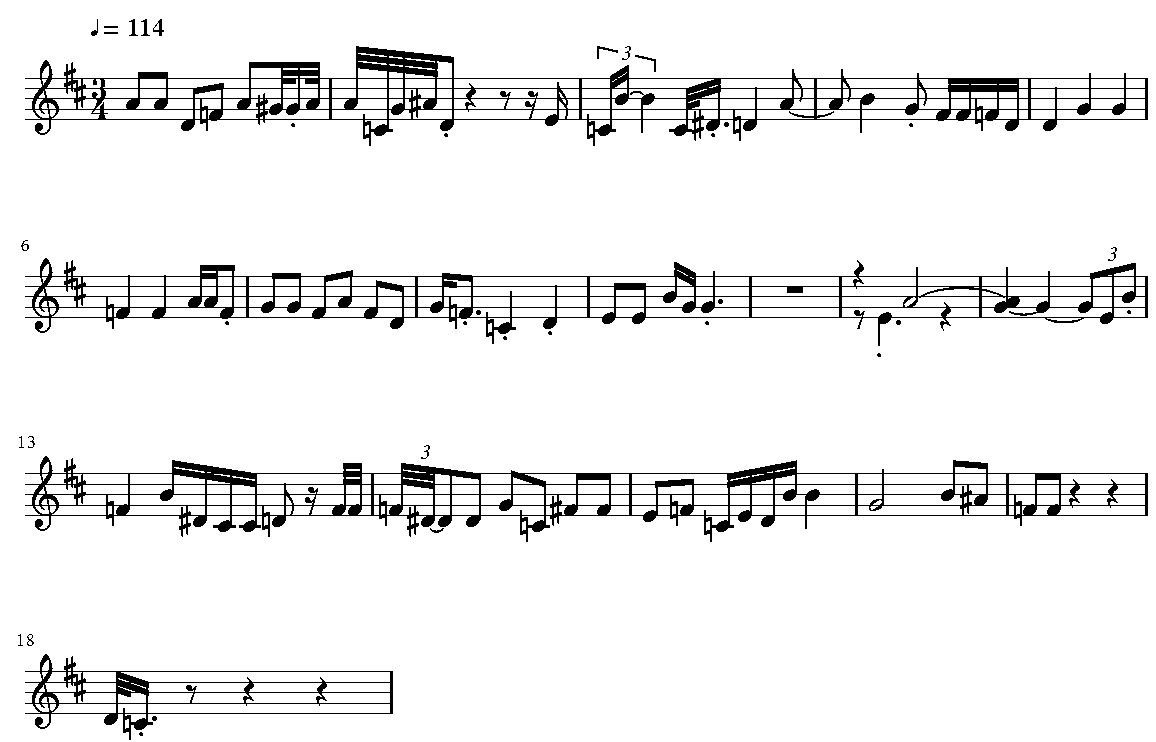
\includegraphics[width=400px]{../images/hmm_melody_generated.pdf}}
\caption{Melody generated with a \ac{HMM}}
\label{ims:hmmmelody}
\end{figure}

Figure \ref{ims:hmmmelody} shows the melody generated with the \ac{HMM}. The resulting melody sounds chaotic and lacks overall structure.

\section{Discussion}
The computational complexity of the forward-backward procedure is $O(T N^2)$. Thus the training time increases greatly as the number of symbols increases and thus it is necessary to constrain the number of symbols as well as the number of states.
\\
Some melodies, especially when the training algorithm was run for a large number of iterations were pleasant. However the results are lacking when compared with those of a higher order Markov chain. A higher order Markov chain has faster training time and the results were as good or better and no good argument could be made to choose the \ac{HMM} for simple melodic generation over a chain.
\\
The power of a \ac{HMM} comes with its hidden states and observations; more complex structures benefit more from this. A better use of the model would be for harmonization or accompaniment. Allan used a \ac{HMM} for harmonization of chorales \cite{Allan2004}. The visible states represent melody notes and the hidden states chords. Such deeper structures are much more meaningful, however since the designed system does not support chords an attempt at harmonization was not made.

\chapter{Instrumental generation with Markov Chains}
\section{Introduction}
For this experiment a compositional engine will be designed that outputs melodies for a specific instrument. 

In order to construct such an instrumental generator an algorithm is required that can predict time-series data.

A large advantage of recurrent neural networks over Markov chains and \acs{HMM} is that neural networks have greater representational power and can take into account syntactic and semantic features. A \ac{RNN} does not make the Markov assumption and is able to take into account long term dependencies.
Markov chains have the advantage of being much simpler to implement and are extremely fast and efficient with the proper implementation. 
Recurrent Neural Networks are more difficult to implement and to train. Various training algorithms exist to train a \ac{RNN}. Training a recurrent neural network is slower than a regular feed forward network. The poor results obtained from the \ac{LSTM} network (See chapter \ref{ch:accomp_lstm}) dissuade us from using them for the instrumental generator.

Markov Chains can also be seen as a special case of a \ac{HMM}. The Markov Chain will be used over a \ac{HMM} as it is simpler and the transition probabilities can be directly calculated.

This concept will utilize Markov Chains to construct a probabilistic model for a sequence of notes. The probability of the next note occurring depends on the previous state of the chain. See section \ref{sec:markov_backround}.

For a Markov Chain of order $m$ the following holds:
\begin{align}
\Pr(X_n=x_n\mid X_{n-1}=x_{n-1}, X_{n-2}=x_{n-2}, \dots , X_1=x_1) =
\\  \Pr(X_n=x_n\mid X_{n-1}=x_{n-1}, X_{n-2}=x_{n-2}, \dots, X_{n-m}=x_{n-m})
\end{align}
For $n > m$

\section{Methodology}
\subsection{General}
For this technique a different Markov Chain will be constructed for each instrument. 
For a certain instrument, all the notes for that instrument in a MIDI file were added to the Markov chain. This chain is used to generate notes according to a certain instrument.
\begin{algorithm}
 \KwData{MIDI files that accord to a certain style}
 \KwResult{Markov Chain for a particular instrument }
 initialization\;
 Choose specific instrument\;
 \For{each MIDI file}{
  \For{each Track}{
    \If{Track instrument is selected instrument}{
     add notes to Markov chain\;
     }{\;
    }
  }
 }
 \caption{Markov Chain for a particular instrument}
 \label{algo:instrumm}
\end{algorithm}

A third order Markov Chain was used. That is, the previous three notes constitute the state of the model. A lower order would result in more novel and random melodies where a higher order would produce melodies with higher similarity. 

For a Markov chain the frequencies of the events can be used to calculate the transition probabilities. For a third order Markov chain the transition probabilities can be calculated by:

\[ a_{i,j} = P(n_i|n_{i-3},n_{i-2},n_{i-1}) = \frac{\text{Count}(n_i, \{ n_{i-3},n_{i-2},n_{i-1} \} )}{\text{Count}(n_i)} \]
where $\text{Count}(n_i, \{ n_{i-1},n_{i-2},n_{i-3} \} )$ is the number of times note $n_i$ occurred after notes $n_{i-3}, n_{i-2}, n_{i-1}$


\subsection{Drums}
The use of a Markov Chain can be expanded to include generation of percussion instruments. 

Percussion instruments in the MIDI standard are a special case and are played on Track channel $10$. Notes played on channel 10 always produce percussion sounds. Each pitch corresponds to a different percussive instrument. Table \ref{tab:percuspitchesexcerpt} displays some of these instruments. The velocity dictates how hard a percussion instrument is hit.

% Table generated by Excel2LaTeX from sheet 'Sheet1'
\begin{table}[htbp]
  \centering
  \caption{Excerpt of some percussion instrument notes in the \ac{MIDI} standard}
    \begin{tabular}{r|r}
    \toprule
    Pitch & Instrument\\
    \midrule
    35    & Bass Drum \\
    38    & Snare Drum \\
    41    & Low Tom \\
    45    & Mid Tom \\
    53    & Ride Bell \\
    54    & Tambourine \\
    \bottomrule
    \end{tabular}%
  \label{tab:percuspitchesexcerpt}%
\end{table}%

In order to train a Markov Chain for a percussive instrument only a small modification is required to algorithm \ref{algo:instrumm}. In place of looping through all tracks only tracks with a channel number of $10$ are used.

\section{Results}
\begin{figure}
\centerline{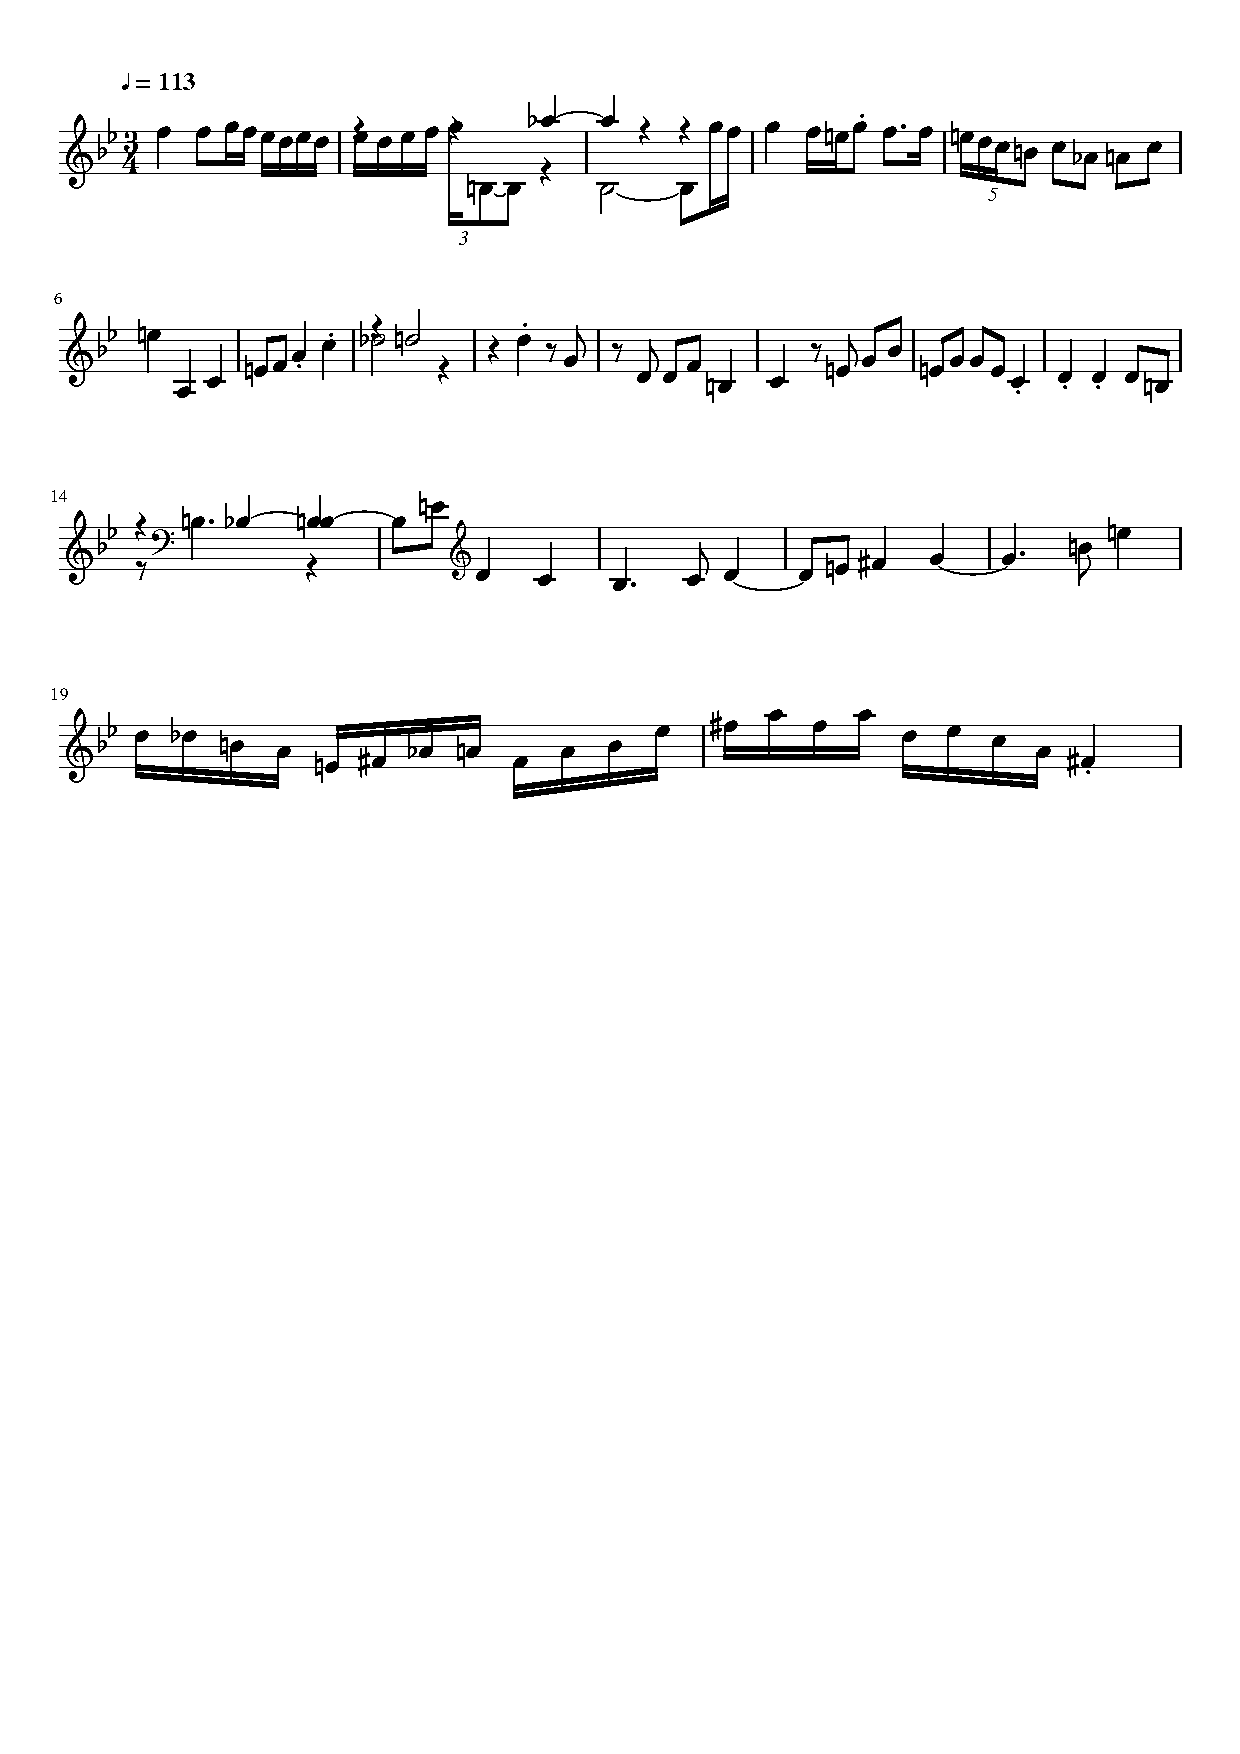
\includegraphics[width=400px]{../images/instrumental_acousticgrand.pdf}}
\caption{Instrumental melody generated with a Markov Chain}
\label{ims:instrumentalmc}
\end{figure}

Figure \ref{ims:instrumentalmc} shows a melody generated with a Markov Chain for the Piano. A third order Markov chain was used with this melody and overall it sounds pleasant. Melodies produced with Markov Chains dont have an overarching theme but do have a local structure and theme.

Melodies produced with Markov Chains are in the same style as the input songs. This reduces compositional value and novelty, especially for higher order Markov Chains. A low order Markov Chain produces more novel although more chaotic and random melodies. 

\section{Potential Improvements}
\begin{itemize}
\item Define which instruments sound good with other instruments
\item Pick which instruments can be slotted together
\item Ensure different tracks accompany each other and are in harmony
\end{itemize}

\chapter{Accompaniment generation with a LSTM network} \label{ch:accomp_lstm}
\section{Introduction}
The \ac{LSTM} network is a \acf{RNN}, however it is more optimized and better suited to classify, process and predict time series in the case when there are long lags of indeterminate length between important events. In this experiment a \ac{LSTM} network is used to generate an accompaniment track for a main melody track

A \ac{RNN} has greater representational power and can take into account syntactic and semantic features. A \ac{RNN} also does not make the Markov assumption and is able to take into account long term dependencies.

\section{Methodology}
The \ac{LSTM} accompaniment is also generated for a specific instrument. 
Since it is difficult to determine which track is the main melody of a composition an assumption is made that the main melody track is the first track found within a \ac{MIDI} file. The accompaniment track is another track within the \ac{MIDI} file.

The LSTM network parameters were set as follows:
\begin{itemize}
\item Activation functions were $\tanh$
\item 2 Input units
\item 15 hidden units
\item 150 output units
\item Learning rate of $0.1$
\item Momentum of $0.9$
\end{itemize}

A list of all possible notes were obtained and the problem was treated as a classification problem. For a set of $n$ possible notes the network has $n$ possible active output units and the active output unit indicates the index of which note was activated. This was done in order to reduce the possibility of incorrect notes as even small error might cause problematic results in alternative representations (if the pitch and duration were used as output).

The input for the neural network is the note pitch and duration of each note in the melody track and the output is the index of the note activated in the accompanied track at the same index. 


$90\%$ of the dataset was used for training and the last $10\%$ was used for verification.

In order to reduce the dimensionality of the output vector filtering is applied. There are bound to be events that occur rarely which can be seen as noise, and the emphasis should be on more prominent notes.
We apply a simple filtering to discard notes which have a normalized frequency below some threshold in the dataset.
\[ \frac{f}{N} < k \]
where f is the frequency of the note, N the total number of notes and k the threshold. Filtering was not applied on rests. 

In the first attempt rests were accounted for. In tracks with a large amount of rests, the regular notes may be filtered out.

\begin{algorithm}
 \KwData{MIDI files that accord to a certain style}
 \KwResult{LSTM training for a particular instrument }
 initialization\;
 \For{each MIDI file}{
  \For{each track other than melody track}{
   \If{instrument is selected instrument}{
  \For{each note in melody track and respective note in accompaniment track}{
      add normalized pitch and -duration of current melody note as inputs to dataset\;
      add output note to list of uniques notes\;
      add output note index as normalized output to dataset\;
     }
    }
  }
 }
 
\caption{Training set for LSTM network}
\end{algorithm}
Since a melody track is stored as a sequence of notes, a note in the melody track and a note in the accompaniment track at the same index might not occur at the same time. Thus we iterate through the melody track and use the note closest in time in the accompaniment track for the algorithm.

Training \ac{LSTM} and other recurrent neural networks is slow, as such the weights and structure of the network are saved to storage and is precomputed for each instrument and style of music.

\subsection{Results}
Since the network requires an input melody track to construct an accompaniment track it does not face the same problems such as lack of structure which most other non-recurrent neural networks do.

The output accompaniment can sometimes be pleasant, however a better timing relation is required between the input and output notes. Most of the produced melodies are repetitive, see figure \ref{ims:lstmaccomp}. The network does not produce an accompaniment which is in harmony or in phase with the main melody track.

\begin{figure}
\centerline{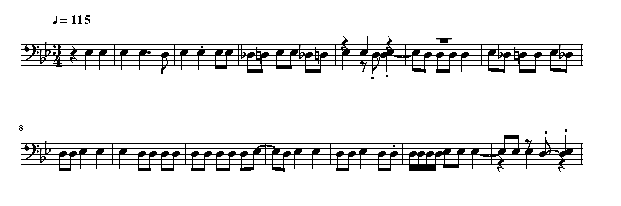
\includegraphics[width=400px]{../images/lstm_accomp.pdf}}
\caption{Accompaniment melody produced with a \ac{LSTM} network}
\label{ims:lstmaccomp}
\end{figure}

Overall the results of the \ac{LSTM} network were average, in comparison with the Markov Chains. A melody generated by the \ac{LSTM} network had better overall structure and theme but were repetitive. Markov chains produced better local melodies.
The poor performance of the \ac{LSTM} network is attributed to the implementation problems and the large training time required for good results.


\chapter{Accompaniment generation with a feed forward network}
\section{Introduction}
In this experiment an attempt is made to generate an accompaniment track for a melody using a feed forward network. One of the reasons for this experiment was to reduce the training time, as recurrent networks have a very large training time. 

\section{Methodology}
For this prototype we construct a neural network with the following parameters:
\begin{enumerate}
\item all units use the sigmoid activation function $\frac{1}{e^{-x}}$
\item 1 input layer, 1 hidden layer, 1 output layer
\item 2 input units
\item 2 output units
\item 10 hidden units
\end{enumerate}

The data for the network consists of the melody track and the accompaniment track. For each note in the melody track the note pitch and duration is given as inputs to the network, the output is the note pitch and duration of the corresponding note in the accompaniment track.

\section{Results}
\begin{figure}
\centerline{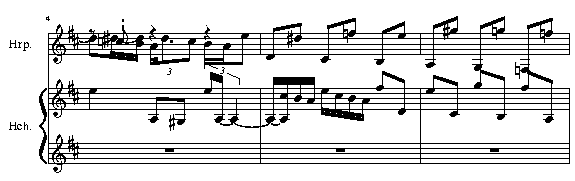
\includegraphics[width=250px]{../images/ann_ff_accomp.pdf}}
\caption{Accompaniment melody produced with a \ac{LSTM} network}
\label{ims:annffaccomp}
\end{figure}

Figure \ref{ims:annffaccomp} shows an accompaniment melody produced with the network.
Since the network does not feature a recurrent topology there was no overall theme or structure. The network learns to output a certain note based on the input. The melodies produced had a better local structure than those produced by the recurrent network. The training speed and execution speed was significantly faster than that of the recurrent network. 
%TODO discuss results

\chapter{Accompaniment generation with a Markov Model}
\section{Introduction}
For this experiment an attempt is made to produce an accompaniment based on the frequency of certain notes occurring in the accompaniment track given the melody track.

More specifically, for each note in the melody track the odds are calculated for each possible accompaniment note that may occur at that time. Given an input melody, for each note in that melody an accompaniment note is produced according to the calculated probabilities. For this the topology of a \ac{HMM} is utilized. A Markov Chain (without transition probabilities) is created and the emission probabilities are calculated.

\section{Methodology}
\begin{algorithm}
 \KwData{MIDI files that accord to a certain style\;}
 \KwResult{Emission frequency table for accompaniment notes\;}
 \For{each MIDI file}{
  Get main melody\;
  \For{each accompaniment track in file\;}{
    \For{each note $N_m,i$ and previous note $N_{m,{i-1}}$ in main melody and corresponding note $N_a,i$ in accompaniment melody\;}
    {
    	Increment frequency of $N_a,i$ in frequency table for $\{N_m,i, N_m,{i-1} \}$\;
    }
  }
 }
 \caption{Constructing frequency table for model}
\end{algorithm}

\begin{algorithm}
 \KwData{Main melody sequence}
 \KwResult{Accompaniment melody sequence }
 initialization\;
 Create empty accompaniment sequence\;
 \For{each note $N_m,i$ and previous note $N_m,{i-1}$ in main melody sequence}{
  	 Lookup frequencies of possible output notes in frequency table for $\{N_m,i, N_m,{i-1} \}$\;
  	 Obtain probabilities for next notes in frequency table\;
  	 Obtain resulting note according to roulette selection\;
  	 Add resulting note to accompaniment sequence\;
    }
 Return accompaniment sequence\;
 \caption{Obtaining accompaniment melody}
 \label{alg:mm_accomp}
\end{algorithm}

\begin{figure}
\centerline{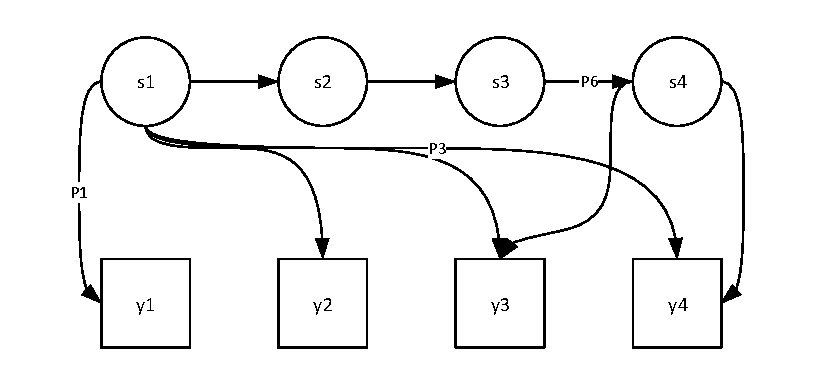
\includegraphics[width=250px]{../images/hmm_illu.pdf}}
\caption{Illustration of a Hidden Markov Model}
\label{ims:hmm_illu}
\end{figure}

Figure \ref{ims:hmm_illu} illustrates a Markov Model. The states $s_i$ denote the notes of the main melody (for a first order Markov Chain) and the states $y_i$ denote the accompaniment notes for melody track. In the case of a \ac{HMM} he states $s_i$ are commonly hidden, however they are known in this case. The states $y_i$ are the output notes that we are interested in generating. 

For this experiment the states are setup up as a second order Markov Chain; that is the next note is determined by the previous two notes. For this model we are not interested in determining thee next state $s_{i+1}$ thus the state transition matrix is not learnt. The emission probabilities of the output notes $y_i$ are learnt instead.

Once the emission probabilities are obtained, we can simply go through the states of the main melody and obtain the emission probabilities at each state. Roulette selection is performed based on the emission probabilities to determine a output note. The output note is then added to the accompaniment sequence. See algorithm \ref{alg:mm_accomp}



\section{Results}
\begin{figure}[h!]
\centerline{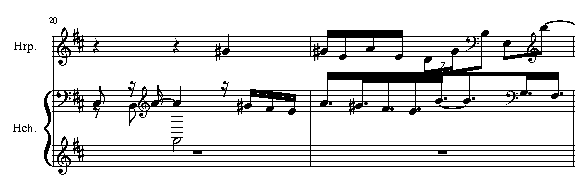
\includegraphics[width=300px]{../images/markov_model_accomp.pdf}}
\caption{Accompaniment generated with Markov Model}
\label{ims:hmm_accomp}
\end{figure}

Accompaniment generation with a Markov Model produces better results than with a \ac{LSTM} network. The states of the model are the notes of the main melody and the observations are the notes of the accompaniment. For a short input melody sequence the resulting accompaniment sounds rather pleasant and fits with the main melody. For longer melodies the accompaniment diverges from the main melody and is not in harmony.




\chapter{Melody generation with Stochastic sampling}
\section{Introduction}
The idea here is to generate a melody from an extant music piece and modifying it to create a new melody. 

Given some model $\lambda$ we modify some piece $p$ into a new piece $p'$ such that $\Pr(p'|\lambda) > P(p|\lambda)$.


In order to modify the piece various sampling methods can be used. The idea is to replace a note of a piece with some other note in an attempt to increase the probability that the new piece come from the model. 

\section{Methodology}
The model to be used will be a simple first order Markov chain. The model is able to evaluate the probability that a music piece or sequence of notes originated from it, i.e. it can calculate $\Pr(p|\lambda)$. The search space for new notes is the set of all notes contained within the Markov chain.
The sampling to be performed is similar to Metropolis sampling. A random note is chosen from piece $p$ and replaced with another note to produce $p'$, the new note is kept if $Pr(p'|\lambda) \geq Pr(p|\lambda)$. The new piece will then be used in subsequent iterations.

\begin{algorithm}
 \KwData{Dataset that accords to a certain musical style}
 \KwResult{Melody Sequence}
 model = MarkovChain()\;
 Add all melody sequences in the dataset to the Markov Chain\;
 Let MaxIter be the maximum number of iterations\;
 iter = 0\;
 Let piece be a random melody sequence from the dataset\;
 \While{iter < MaxIter}{
 	 iter = iter + 1\;
 	 random\_index = Random number between 0 and number of notes in piece\;
 	 Let new\_note be a random note in the search space\;
 	 new\_piece = piece.ReplaceNote(random\_index, new\_note)\;
	 \If{ model.Probability(\text{new\_piece}) >= model.Probability(\text{piece})}{
 	 	piece = new\_piece\;
 	 }
    }
 Return piece\;
 \caption{Pseudocode for generating a melody using Stochastic Sampling}
\end{algorithm}

\section{Results}
\begin{figure}[h!]
\centerline{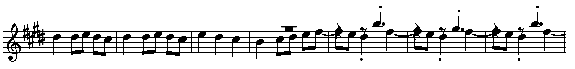
\includegraphics[width=300px]{../images/swr_in.pdf}}
\caption{Randomly selected input melody 1}
\label{ims:swr_in}
\end{figure}

\begin{figure}[h!]
\centerline{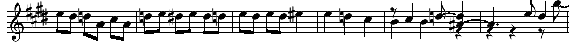
\includegraphics[width=300px]{../images/swr_out.pdf}}
\caption{Output melody using the stochastic sampling on melody 1}
\label{ims:swr_out}
\end{figure}

\begin{figure}[h!]
\centerline{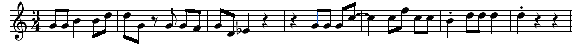
\includegraphics[width=300px]{../images/swr_in2.pdf}}
\caption{Randomly selected input melody 2}
\label{ims:swr_in2}
\end{figure}

\begin{figure}[h!]
\centerline{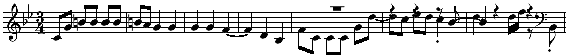
\includegraphics[width=300px]{../images/swr_out2.pdf}}
\caption{Output melody using the stochastic sampling on melody 2}
\label{ims:swr_out2}
\end{figure}

Figure \ref{ims:swr_in} shows the randomly selected melody used to generate the melody in figure \ref{ims:swr_out} using stochastic sampling with replacement. The number of iterations for the first melodies were $100$.
Using a larger number of iterations of $200$ more variety and change can be seen. Figure \ref{ims:swr_in2} shows the randomly selected melody used to generate the melody in figure \ref{ims:swr_out2} using the larger number of iterations.


\section{Conclusion}
The problem with this method is that it might not seem creative, even though it can produce interesting pieces. Another problem is that it might fall in a local minimum, where further replacements cannot improve the probability of the piece. Lastly since a first order Markov Model was used to calculate the probability of the piece it could not always produce changes which had a overall theme. Some changes felt out of place.
Overall the method produced pleasing results and indicates that modifications to existing pieces can be a efficient way to generate new pieces in a certain style.

In order to improve this method a different of more accurate model could be used other than the first order Markov chain. A \ac{HMM} might yield better results.
\part{Detail Design}
%!TEX root = ../Report.tex
%************************************************

% Detail design

\chapter{Introduction}
In this part the design of the end user application will be discussed in detail. Topics covered include the final selection of algorithms in the application, the design of the user interface, a high level overview of the data structures used, the functionality and features of the application and finally some additional considerations will be reviewed.

\chapter{Technology, Platform and Programming Language}
\section{Introduction}
Some algorithms and features lend themselves to being implemented more easily in certain languages than other. A programming language needs to be chosen that does not restrain the functionality of the application. 
The four languages with most support include:
\begin{enumerate}
\item Python
\item C\# (and other .NET languages)
\item Java
\item C++
\end{enumerate}

Machine learning libraries exist for all of the above mentioned languages. Python has poor support for rich user interfaces. Java is a good contender and is cross platform. Haskell has strong expressiveness and powerful language features.

\section{Trade-off study}

Thus in order to make a final selection a trade off study was conducted. Additional factors included in the trade-off study were the expressiveness and amount of features in a language and the cross platform compatibility. These features have a lower weighing.
Consideration is made to the end user and the user interface support is given the highest weighing.  

Thus the factors considered are:
\begin{itemize}
\item Development speed - Estimated amount of programmer time required in each language.
\item Available support and help - How easy it is to obtain help and support
\item Available machine learning and pattern recognition libraries. Implementation of some algorithms prove difficult.
\item \ac{UI} design and libraries - Availability of libraries to design a good user interface and experience
\item Cross platform compatibility - How well does the language, features and libraries run on other platforms
\item Expressiveness and features - Language features which ease development. Expressive languages facilitate advanced data structures and algorithms in few \ac{LOC}
\end{itemize}

% Table generated by Excel2LaTeX from sheet 'Sheet1'
\begin{table}[htbp]
  \centering
  \caption{Programming languages trade-off study}
    \begin{tabular}{rr|rrrrr}
    \toprule
          & Weight & C\#   & Java  & Python & C++   & Haskell \\
    \midrule
    Development speed & 0.5   & 8     & 7     & 8     & 5     & 9 \\
    Available support and help & 0.2   & 8     & 8     & 8     & 6     & 4 \\
    Machine learning libraries & 0.4   & 6     & 8     & 9     & 8     & 4 \\
    \acs{UI} design and libraries & 0.6   & 10    & 8     & 5     & 7     & 3 \\
    Cross platform compatibility & 0.2   & 6     & 10    & 10    & 10    & 10 \\
    Expressiveness and features & 0.4   & 7     & 6     & 8     & 5     & 10 \\
    \midrule
    Total & 2.3   & 18    & 17.5  & 17.4  & 15.1  & 14.7 \\
    \bottomrule
    \end{tabular}%
  \label{tab:languagetradeoff}%
\end{table}%

\section{Discussion}
Winner: \emph{C\#}\footnote{The algorithmic code is cross platform and can be run through Mono, even though the graphical front end developed in \ac{WPF} cannot.}

.NET languages facilitate the use of \ac{WPF} - a graphical system for rendering user interfaces, which will allow a rich user experience to be developed. Java and Python are good contenders.

C\# additionally has the following advantages:
\begin{enumerate}
\item Ability to easily create rich user interfaces.
\item C\# runs on the CLR and allows access to the large .NET library\footnote{Additionally the IKVM project allows access to Java libraries}
\item Powerful language constructs such as operator overloading, event handling, delegates, powerful multi-threading support and generics.
\end{enumerate}


\chapter{Selection of algorithms}
\section{Introduction}
In this chapter the selected algorithms for the end user application are chosen.
The algorithms for consideration are:
\begin{enumerate}
\item Melody generation with Genetic Algorithms.
\item Melody generation with Hidden Markov Models.
\item Accompaniment generation with Hidden Markov Models.
\item Accompaniment generation with a \ac{LSTM} network.
\item Accompaniment generation with a feed forward \ac{ANN}.
\item Instrumental generation with Markov Chains.
\end{enumerate}

The selection of algorithms will be done by means of elimination. Algorithms that yielded sub minimum results will not be selected for inclusion into the end user application.

\section{Trade-off studies}
For the final end-user application only a subset of algorithms will be chosen. In order to quantitatively select good algorithms a trade-off study will be done on the investigated algorithms. The factors considered are:
\begin{itemize}
\item Training time - The amount of time taken to train the algorithm on initial data.
\item Generation time - The amount of time the algorithm takes to produce a melody after it is trained.
\item Flexibility - How well the algorithm can accommodate different input data. How easily it can be extended or modified.
\item Pleasantness - Subjective measure of good a melody is.
\end{itemize}
% Table generated by Excel2LaTeX from sheet 'Sheet2'
\begin{table}[htbp]
  \centering
  \caption{Trade-off study for algorithms for melody generation}
    \begin{tabular}{rr|rrrr}
    \toprule
    \multicolumn{6}{c}{Melody generation} \\
    \midrule
          & Weight & GA    & FFANN & MC    & HMM \\
    \midrule 
    Training time & 0.3   & 10    & 4     & 8     & 5 \\
    Generation time & 0.6   & 4     & 7     & 8     & 7 \\
    Flexibility & 0.6   & 10    & 7     & 6     & 6 \\
    Pleasantness & 0.7   & 5     & 4     & 7     & 5 \\
          &       &       &       &       &  \\
          \bottomrule
    Total & 2.2   & 14.9  & 12.4  & 15.7  & 12.8 \\
    \bottomrule
    \end{tabular}%
  \label{tab:tomelgen}%
\end{table}%

Table \ref{tab:tomelgen} shows the trade-off study for algorithms for melody generation. Melody generation is simply the generation of a single track consisting of a list of notes. From the trade-off study we can see that the \ac{HMM} and \ac{FFANN} performed poorly and thus will not be selected.

% Table generated by Excel2LaTeX from sheet 'Sheet2'
\begin{table}[htbp]
  \centering
  \caption{Trade off study for algorithms for accompaniment generation}
    \begin{tabular}{rr|rrrr}
    \toprule
    \multicolumn{6}{c}{Accompaniment generation} \\
    \midrule
          & Weight & HMM   & FFANN & MM    & LSTM \\
    \midrule  
    Training time & 0.3   & 6     & 4     & 8     & 3 \\
    Generation time & 0.6   & 7     & 7     & 8     & 6 \\
    Flexibility & 0.6   & 6     & 7     & 6     & 5 \\
    Pleasantness & 0.7   & 3     & 5     & 6     & 3 \\
          &       &       &       &       &  \\
          \bottomrule
    Total & 2.2   & 11.7  & 13.1  & 15    & 9.6 \\
    \bottomrule
    \end{tabular}%
  \label{tab:toaccompgen}%
\end{table}%

Table \ref{tab:toaccompgen} indicates the trade-off study for algorithms for accompaniment generation. Accompaniment generation is a list of notes that have to accompany the main melody. From the trade-off study we can see that the \ac{HMM} and \ac{LSTM} performed poorly and thus will be excluded from the main application.

% Table generated by Excel2LaTeX from sheet 'Sheet3'
\begin{table}[htbp]
  \centering
  \caption{Comparison of frequency metric time and pleasantness}
    \begin{tabular}{r|rr}
    \toprule
          & Time (ms) & Pleasantness \\
    \midrule
    Chromatic Tone & 8992  & 4 \\
    Chromatic Tone Distance & 11017 & 5 \\
    Chromatic Tone Duration & 13688 & 5 \\
    Melodic Bigram & 3900  & 5 \\
    Melodic Interval & 9037  & 5 \\
    Pitch & 14001 & 4 \\
    Pitch Distance & -     & - \\
    Rhythm & 367   & 4 \\
    Rhythmic Bigram & 4729  & 7 \\
    Rhythmic Interval & 5501  & 6 \\
    \bottomrule
    \end{tabular}%
  \label{tab:fmetrictimepleasant}%
\end{table}%


For the frequency metrics to be used with the cosine similarity fitness function we refer to table \ref{tab:metriccomp}. The pleasantness and time for each metric is repeated in table \ref{tab:fmetrictimepleasant} for convenience. The Pitch Distance metric was excluded as it took too long. The chromatic tone, pitch and rhythm metrics will also be excluded as all scored low pleasantness. 


\section{Conclusion}
From the trade-off study the selected algorithms were chosen.
In summary, the selected algorithms for the end-user application were:
\begin{enumerate}
\item Genetic Algorithms for melody generation.
\item Markov Chains for melody generation (with percussion support).
\item Feed Forward Artificial Neural Network for accompaniment generation.
\item Markov Model for accompaniment generation.
\end{enumerate}

Only the cosine similarity fitness function will be used, as the \ac{NCD} fitness function performed poorly. The metrics for the cosine similarity fitness function were selected as:
\begin{enumerate}
\item Chromatic Tone Distance
\item Chromatic Tone Duration
\item Melodic Bigram
\item Melodic Interval
\item Rhythmic Bigram
\item Rhythmic Interval
\end{enumerate}

Using trade-off studies the worst results were eliminated from all algorithms.

\chapter{Features and Functionality}
The main goal of the application is to generate melodies according to a certain styles. The user is to select a certain category of music and the application will generate a musical piece in that style. The premise is to generate the melodies in a certain style using machine learning techniques that will use the data present in the corpus of MIDI files. 

Since training machine learning algorithms take up a lot of time it is not feasible to train the algorithm on the fly. Training will take place beforehand and the resulting data structure of the algorithm will be cached to a file. 
For example a Neural Network will save its topology and weights to a file; this allows the application to load the file, present inputs to the neural network and output a result without spending time learning the optimal weights for the network.

Additional features would be to allow the user to save a generated melody to a file (in \ac{MIDI} or a custom file format), load and play an existing \ac{MIDI} file (for comparison or other aims), re-randomize a generated composition and view more information or properties of the generated music piece.

The application is to be used by end users which do not have background on machine learning. The application is to be as user-friendly as possible while still having flexibility in composing songs. The user interface is to visually display the song and playback of it. Playback functionality such as playing and stopping a song are mandatory.

To summarize, the application will:
\begin{enumerate}
\item Implement the selected algorithms and allow them to be used for song generation.
\item Allow saving and loading of \ac{MIDI} files
\item Generate a monophonic melody according to a certain style. Allow the user to select which algorithm to use and adjust high level parameters
\item Playback functionality including playing, pausing and stop a song. 
\item Feature a user friendly interface.
\item Visually display the generated melody.
\item Allow the user to randomize the song based on the selected settings.
\item Cache machine learning data to improve performance of the application.
\end{enumerate}

\chapter{Graphical user interface}

\section{Introduction}

In this chapter the design of the graphical user interface is presented, along with the features and functionality of the application.

As mentioned above the user interface is to have the following features
\begin{itemize}
\item Visually display the generated song.
\item Selecting the category of melodies to be generated.
\item Select algorithm and high level parameters.
\item Buttons to allow for saving, loading, pausing, pausing, stopping and playing of songs.
\end{itemize}

The user interface will be developed using \ac{WPF} and \ac{XAML}.

\section{Playback}

\begin{figure}
\centerline{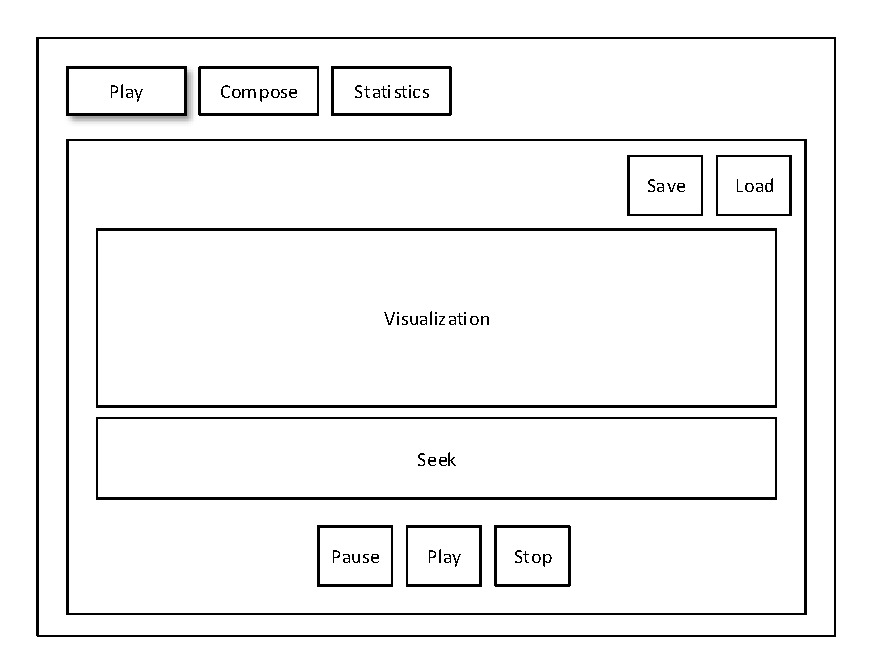
\includegraphics[width=400px]{../images/ui_play.pdf}}
\caption{User interface for playback functionality}
\label{ims:uiplay}
\end{figure}



Figure \ref{ims:uiplay} indicates the starting interface of the application. This interface provides controls for playback functionality, is responsible for displaying a visual of the song being currently played, provides saving and loading functionality and allows the user to randomize the current song using the parameters set in the compose view.

\section{Composition}
\begin{figure}
\centerline{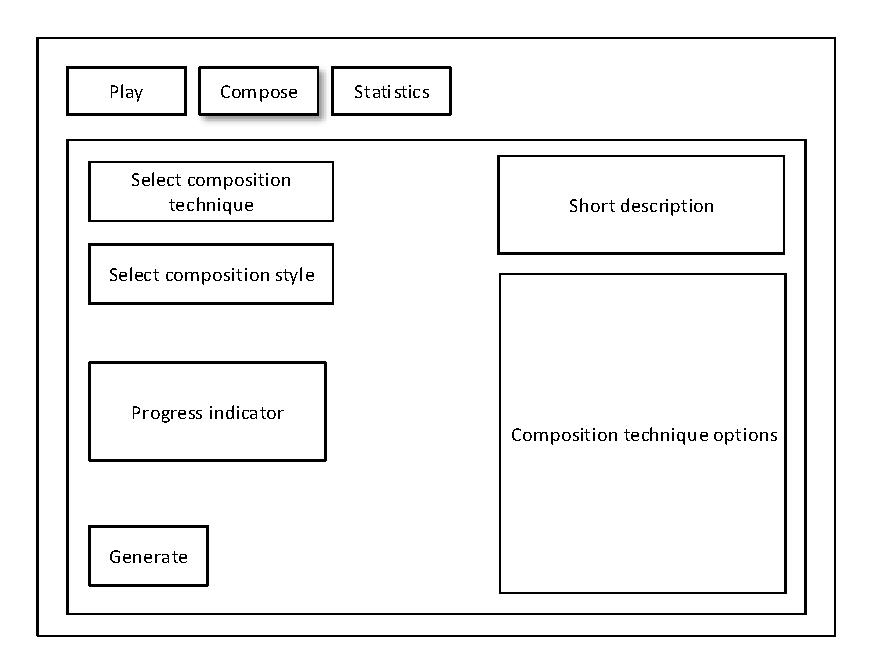
\includegraphics[width=400px]{../images/ui_compose.pdf}}
\caption{User interface for composition functionality}
\label{ims:uicompose}
\end{figure}


The interface as shown in figure \ref{ims:uicompose} allows the user to select the music style or category for music to be generated in. A track is a sequence of notes played in a particular instrument. A user is able to add new tracks using the provided button, which takes them to a new window as in figure \ref{ims:uitrack}. If a user double clicks on a specific track the frequency metrics of the track are shown as in figure \ref{ims:uimetrics}.


\section{Track generation}

Figure \ref{ims:uitrack} allows the user to generate a track using a specific technique. This interface allows the user to select the type of technique for track generation and also displays the progress. Once a track is generated it can be added to the list of tracks as in figure \ref{ims:uicompose}.

\begin{figure}
\centerline{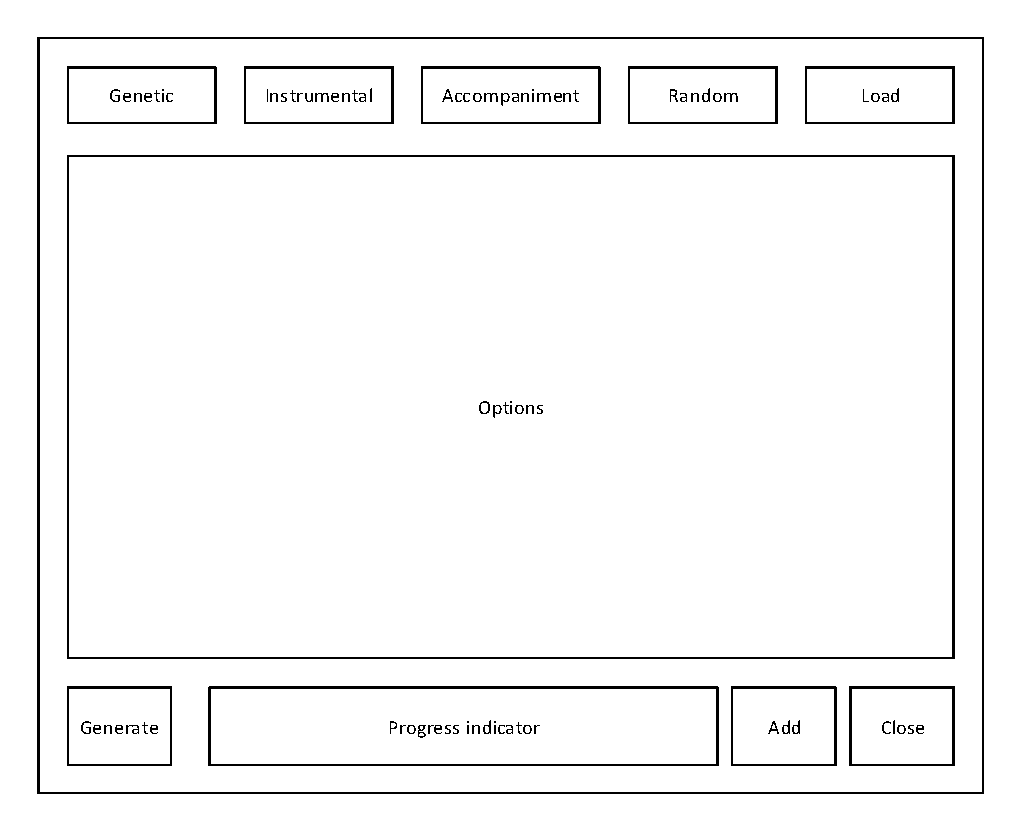
\includegraphics[width=400px]{../images/ui_track.pdf}}
\caption{User interface for melody generation}
\label{ims:uitrack}
\end{figure}



\section{Statistics}

Figure \ref{ims:uimetrics} displays a list of frequency metrics about the track selected. An example metric is the frequency of musical intervals within a melody ($\text{mi} = |p_i - p_{i-1}|$, where $p_i$ is the pitch at index $i$); more information about frequency metrics can be found in section \label{chap:metrics}.

\begin{figure}
\centerline{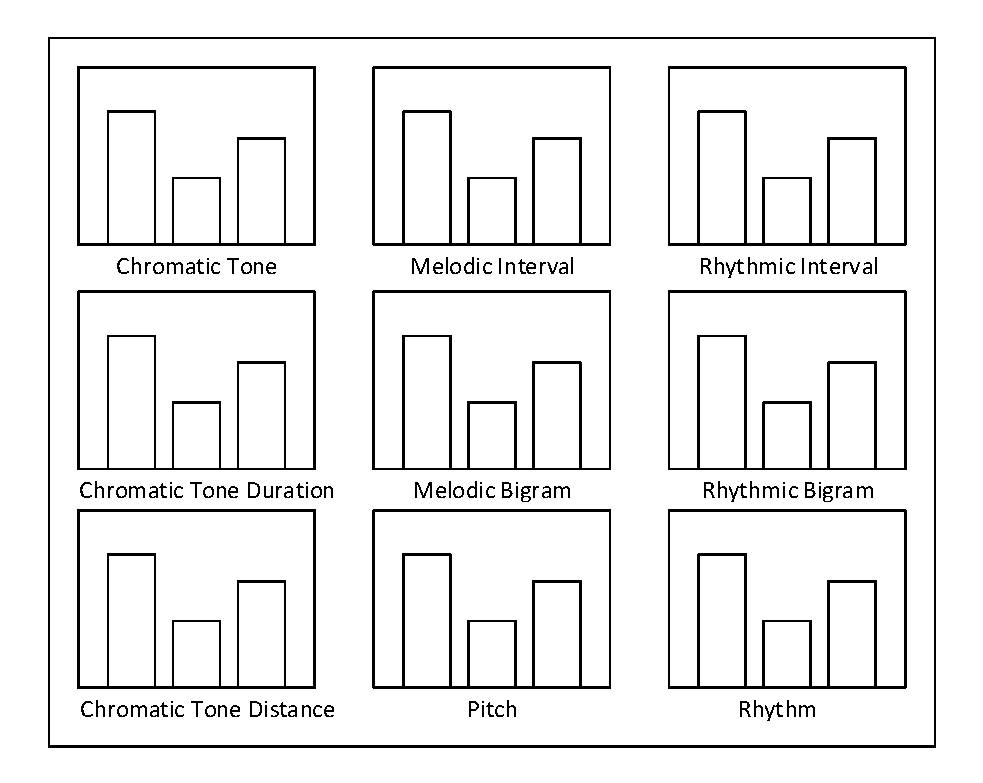
\includegraphics[width=400px]{../images/ui_metrics.pdf}}
\caption{User interface for displaying metrics of a melody}
\label{ims:uimetrics}
\end{figure}

 
\section{Visualization}
The visualization blocks in figures \ref{ims:uicompose} and \ref{ims:uitrack} will be a simple visual displaying the notes over time. 

%A simplified music sheet representation will be used, something in the vein of figure \ref{ims:uiharrymusicsheet}.

\begin{figure}
\centerline{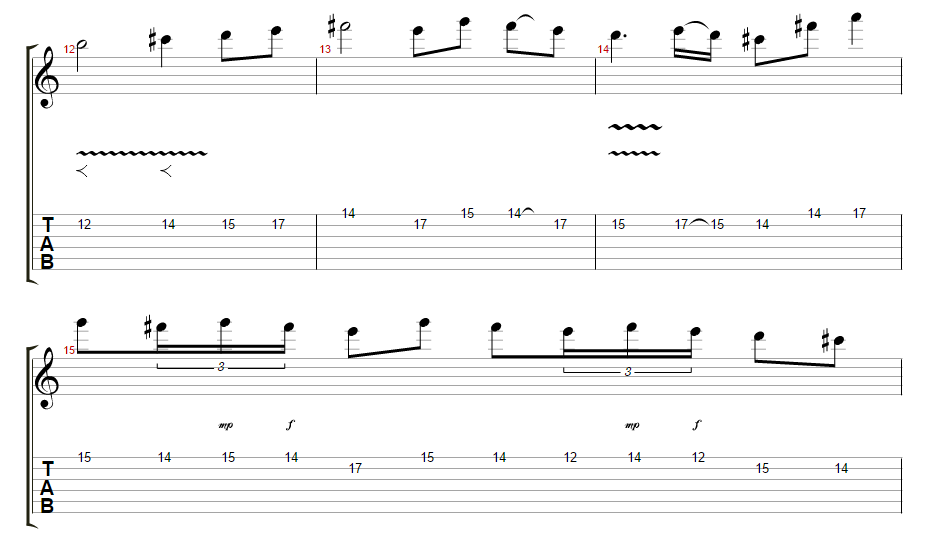
\includegraphics[width=400px]{../images/alphatab_example.png}}
\caption{Example of a music sheet rendered with alphatab}
\label{ims:alphatab}
\end{figure}

AlphaTab is a cross platform music notation and guitar tablature rendering library. It is the only music notation library available on C\# which will fit the need for visualization of notes required.
Figure \ref{ims:alphatab} indicates a music sheet rendered with Alphatab. Note that Alphatab is geared towards guitarists and provides a lot more information which is unwanted for a simple visualization. 

Since the library is open source it will be modified to suit our needs. Guitar tabs, timing information, lyrics and any other excessive information will be removed. In addition it is necessary to show which note is currently played when a melody is played. The active note will be displayed in red.

\begin{figure}
\centerline{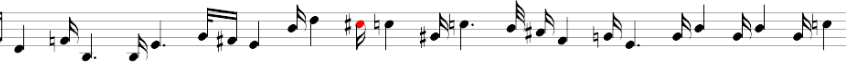
\includegraphics[width=300px]{../images/music_sheet_visualization.png}}
\caption{Desired notes visualization}
\label{ims:uiharrynotesvisualization}
\end{figure}

Figure \ref{ims:uiharrynotesvisualization} displays the designed simple notes visualization required for the application. Alphatab will be modified in order to produce a result similar to this.


%\begin{figure}
%\centerline{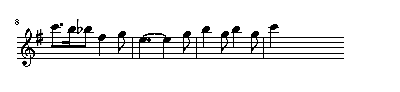
\includegraphics[width=400px]{../images/ui_visualization.pdf}}
%\caption{Visualization of notes}
%\label{ims:uiharrymusicsheet}
%\end{figure}



\section{State control}

\begin{figure}
\centerline{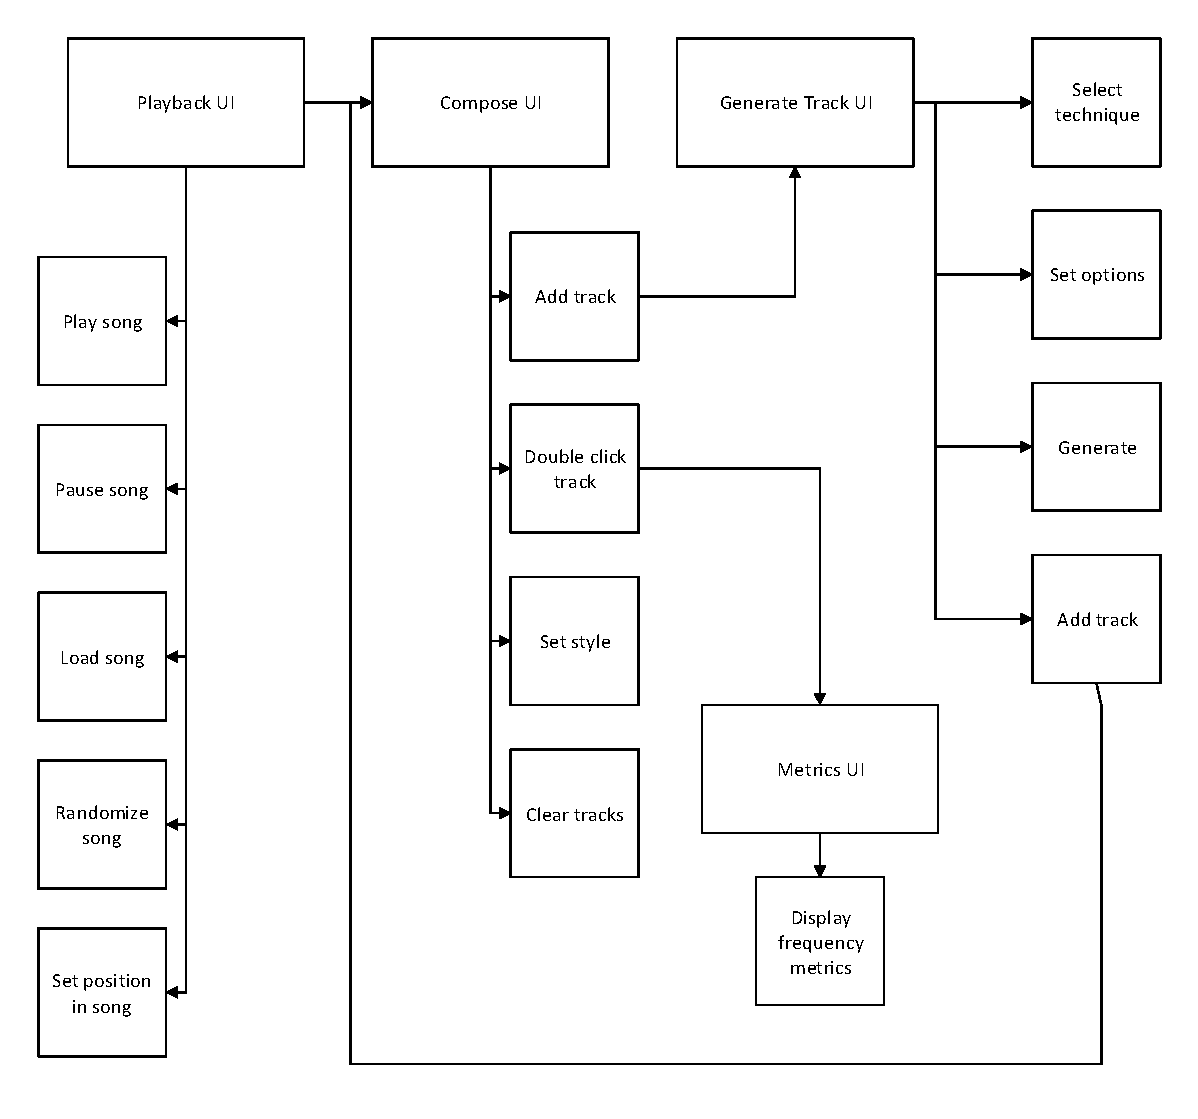
\includegraphics[width=400px]{../images/ui_control_blockdiagram.pdf}}
\caption{State diagram of the user interface}
\label{ims:uiflow}
\end{figure}

Figure \ref{ims:uiflow} shows the state diagram of the user interface. 
From the figure it can be seen that the Playback UI controls playback of a single composition. From the composition UI the necessary tools and functionality can be accessed to create new melodies.


% Functionality and features
% Design
\chapter{Final considerations}
\part{Denouement}
%!TEX root = ../Report.tex
%************************************************

% Detail design

\chapter{Results}
This chapter outlines the results, including the design of the user interface, functionality of the application and a short summary of the results of the incorporated algorithms.
The majority of the results have already been covered in part \ref{part:algo}, however a discussion is provided.

\section{User interface}

\begin{figure}
\centerline{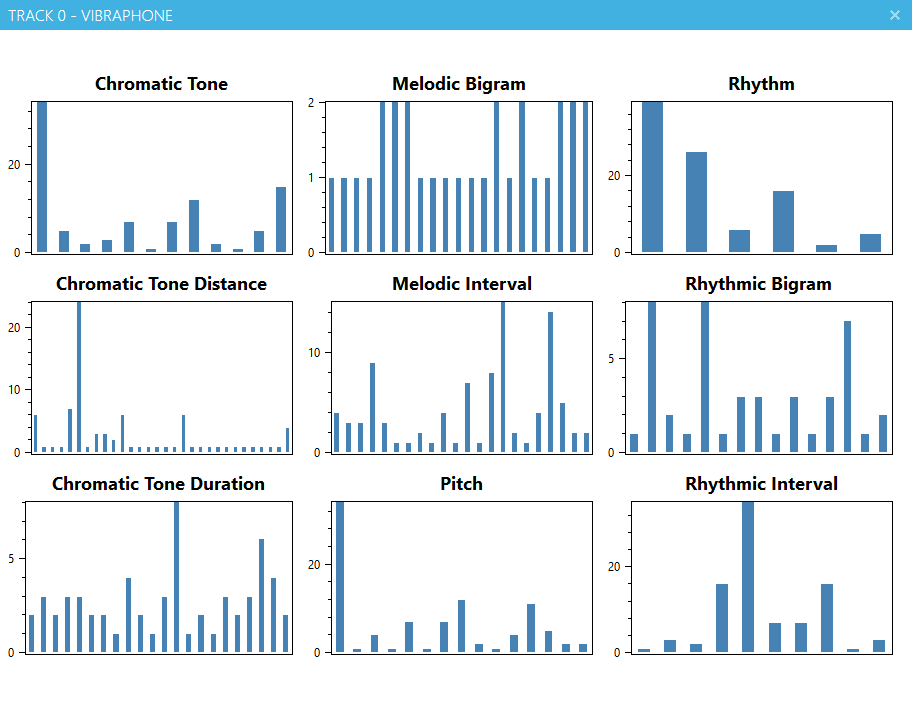
\includegraphics[width=400px]{../images/res_ui_metrics_harry_t0.png}}
\caption{Frequency metrics for the first track Harry Potter Opening Theme Song}
\label{ims:metricsharryt0}
\end{figure}

Figure \ref{ims:metricsharryt0} shows the frequency metrics for the first track of the Harry Potter opening theme song.

\begin{figure}
\centerline{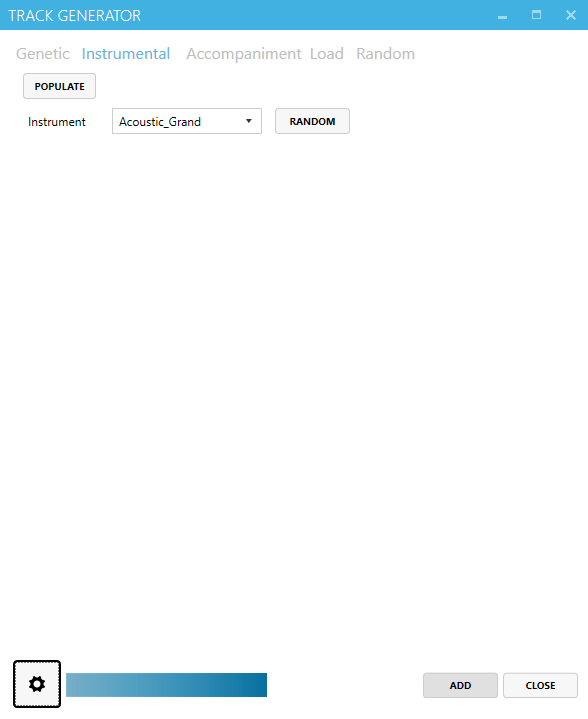
\includegraphics[width=400px]{../images/res_ui_track_generator_instr.png}}
\caption{Window of instrumental tab in track generator}
\label{ims:uitrackgeninstr}
\end{figure}

Figure \ref{ims:uitrackgeninstr} indicates the window of the track generator with the instrumental tab selected. Here a Markov Chains generates a instrumental melody for the Acoustic Grand instrument.


\chapter{Conclusion}
The aim of this project was to design an application that is able to compose melodies in a certain musical style using machine learning algorithms. A brief survey was done on existing attempts to compose melodies using machine learning techniques.
\\

Evolutionary algorithms are versatile and are well suited to the the task of musical composition. The task of designing a good fitness function for a genetic algorithm is rather formidable.
Musical composition is a emotional human process and is subjective in nature. This makes formalization of what constitutes a good melody difficult. 
An attempt was made by using the \ac{NCD} to rate the fitness of melodies, however the results were not satisfactory.
Decent results were obtained by using frequency metrics in conjuction with a similarity measure. This approach provides high fitness to individuals which have similar statistical properties to the target piece. The problem with the approach is that a high statistical similarity may be achieved but this does not necesarily imply that a individual will be perceived as pleasant or good.
\\

A different approach was taken thereafter, other than relying on statistical properties and requiring a function to quantify the pleasantness of a melody. A probalistic approach was taken to predict the pattern of melodies. By employing the Markov property - the probability distribution of future states depend only upon the present states simplifications can be made and Markov Models can be designed. The simplest Markov Model, the Markov Chain produced pleasant results. A third order Markov Chain, where the next note is determined by the preceeding 3 notes produced pleasant results without sacrificing too much novelty and avoiding too much similarity. By employing another Markov Model, attempt was made to produce an accompaniment for a melody, by calculating the probilities for an accompaniment note by the preceeding 2 notes in the melody track. This Markov Model also yielded satisfactory results however more work is required on timing and synchronization.
Overall these probalistic models yield good results, however the melodies produce lack an overarching theme and structure. Furthermore since Markov Models a input dataset and calculate the transmission and emission probabilities based on the input data the novelty and composition value are low. These models produce pleasant results but are not creative or original.
\\

Further works is needed to develop an algorithm that is able to compose melodies that have an overarching theme or structure.  Further work can be done using recurrent neural networks in a variety of topologies or using a custom Hidden Markov Models. These techniques were used in a simplistic way to generate the accompaniment to a melody with acceptable results.
\\

The results of most the algorithms could be improved by incorporating domain knowledge into the system. Musical knowledge could constrain the algorithm to produce more acceptable results. A hybrid system that incorporates expert knowledge may reduce the number of unpleasant patterns produced and improve note transitions and so forth.
\\

The application used a number of simplifications. A major simplification was that only monophonic melodies were considered, no chords. A more advanced system can be designed that applies the investigated algorithms to chords as well. Further algorithms could be used for harmonization.
\\

The application conforms to the specifications and is able to satisfactorily produce melodies in Classical, Jazz, Drum and Video Games styles using Markov Chains, Neural Networks and Genetic Algorithms.

\chapter{Future Work}
\cleardoublepage
%\ctparttext{You can put some informational part preamble text here. 
%Illo principalmente su nos. Non message \emph{occidental} angloromanic
%da. Debitas effortio simplificate sia se, auxiliar summarios da que,
%se avantiate publicationes via. Pan in terra summarios, capital
%interlingua se que. Al via multo esser specimen, campo responder que
%da. Le usate medical addresses pro, europa origine sanctificate nos se.}

%\part{The Showcase}
%%!TEX root = ../Report.tex
%************************************************
\chapter{Music and music-representation}\label{ch:introduction}
\section{Musical elements}
Music is an art form for which the medium is sound.
The common elements in music are:
\begin{itemize}
\item Pitch - Subjective sensation reflecting lowness and highness of sound, also represented more objectively as frequency.
\item Rhythm - Arrangement of sounds and silences.
\item Dynamics - Execution of a given piece (speed, volume)
\item Timbre - Tone
\end{itemize}

Music composition refers to the creation and recording of music through a medium that others can interpret.  Music can be composed for repeated playback or it can be composed on the spot.

A melody is a set of notes (or rests) that are performed in series. Each note may have a different length and different stress. These notes are arranged in a certain rhythmic pattern.

Notes were traditionally given a letter to represent the pitch of the note. The names come from the set $\{A, B, C, D, E, F\}$. Notes may have their pitch modified by additional symbols such as a sharp($\#$).

Notes and rests may have different lengths.


Li and Sleep have found that a given piece of music remains recognizable when the length of the notes are randomized \cite{Ling2004}.

\section{Midi}
Music can be stored digitally in a variety of formats and encodings. This allows repeated performance of the same track and also eases distribution of the music.

\ac{MIDI} is a standard which describes the protocol, digital interface and connectors that allows electronic instruments to communicate with one another.

The \ac{MIDI} 1.0 detailed specification fully describes the \ac{MIDI} interface \cite{MIDIManufacturersAssosciation1995}

The \ac{MIDI} file format describes the way \ac{MIDI} information is stored in a file. Each \ac{MIDI} file starts with a header chunk that describes the time division and the number of tracks. After the header chunk multiple track chunks occur. Each track contains multiple \ac{MIDI} events.

The header chunk is described as follows:
\begin{lstlisting}
"MThd" + [header_length] + [format] + [n] + [division]
\end{lstlisting}
where
\begin{acronym}
\item{[header\_length]} always 6 bytes
\item{[format]} 0 - single track format, 1 multiple track format, 2 multiple song format
\item{[n]} number of track chunks
\item{[division]} unit of time for delta timing
\end{acronym}

After the header chunk [n] track chunks follow.
Each track chunk is composed as follows:
\begin{lstlisting}
"MTrk" + [length] + [track_event] <+ [track_event1] + [track_event2] + [...] + [track_eventn]>
\end{lstlisting}
where
\begin{acronym}
\item{[length]} number of bytes in track chunk
\item{[track\_event]} sequenced track event, described next
\end{acronym}

The track chunk can be seen to contain multiple track events.
Each track event consists a delta time and either a midi event, meta event or sysex\_event:
\begin{lstlisting}
[v_time] + [midi_event] | [meta_event] | <sysex_event>
\end{lstlisting}
The meta-event contains additional information such as text which can be displayed, instrument names, lyrics and so on.

% Table generated by Excel2LaTeX from sheet 'Sheet1'
\begin{table}[htbp]
  \centering
  \caption{Table containing some midi events}
    \begin{tabular}{rrrrr}
    \toprule
    \multicolumn{1}{c}{\textbf{Command}} & \multicolumn{1}{c}{\textbf{Meaning}} & \multicolumn{1}{c}{\textbf{parameters}} & \multicolumn{1}{c}{\textbf{param 1}} & \multicolumn{1}{c}{\textbf{param 2}} \\
    \midrule
    0x80  & Note-off & 2     & key   & velocity \\
    0x90  & Note-on & 2     & key   & velocity \\
    0xA0  & Aftertouch & 2     & key   & touch \\
    0xB0  & Continuous controller & 2     & controller \# & controller value \\
    0xC0  & Patch change & 2     & instrument \# &  \\
    0xD0  & Channel Pressure & 1     & pressure &  \\
    \bottomrule
    \end{tabular}%
  \label{tab:midievents}%
\end{table}%

Table \ref{tab:midievents} shows some of the possible midi events. Each event has a command and additional arguments. Note-on and note-off are the two more important events in the table and indicate how long a note is played. 

The full midi specification can be ordered online at \href{http://www.midi.org/}{midi.org}\footnote{http://www.midi.org/}


\section{Representation}
Representation of music is important to achieve successful generation of a correct solution \cite{gibson1991neurogen}. However the search space of machine learning algorithms may be too large if limitations are not introduced \cite{Jacob1995}. 

\begin{figure}
\centerline{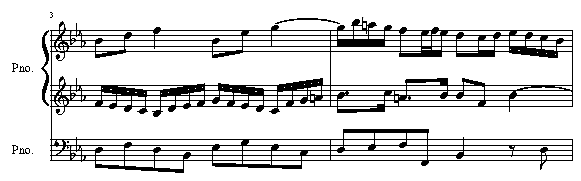
\includegraphics[width=400px]{../images/bwv05225_excerpt.pdf}}
\caption{Excerpt of Bach's BWV 05225}
\label{ims:be05225}
\end{figure}

Figure \ref{ims:be05225} shows the music sheet of an excerpt of Bach's BWV0525 Sonata using modern notation. 

The musical data from musical pieces need to have a proper representation in order to be used by a machine learning algorithm.

In \cite{Eck2002} Eck a form of 12-bar blues was used with 8 notes per bar. 
He used the following representation for the \acs{LTSM} system:
\begin{enumerate}
\item 12-bar musical pieces were used
\item 8 notes per bar were used
\item The same chords were used between songs, see figure \ref{ims:eckchords}
\item The melody notes were built using the pentatonic scale
\item The neural network inputs indicate whether a certain note is on or off
\end{enumerate}

A melody would be represented differently in a linear genetic algorithm.
A simple melody consisting only of a few notes could be represented as seen in figure \ref{ims:ga_melody}. Note the duration of a note is not defined and could be consider fixed.

However it might be preferable to encode more events such rests, chords, dynamics, note duration and so on.

Tree based representations are found in genetic programming \cite{Langdon2008}. Minsky has argued that tree representation is more suited to music as it mimics the hierarchical structure that is found in music \cite{Minsky1992}.

A melody could be represented in tree form as seen in figure \ref{ims:gp_melody}. The bottom leaves denote the pitch and duration. The higher level nodes perform operations.


\begin{figure}
\centering
\begin{minipage}{.5\textwidth}
  \centering
  \includegraphics[width=180px]{../images/ga_melody.png}
  \caption{Simple melody represented as a bit string}
\label{ims:ga_melody}
\end{minipage}%
\begin{minipage}{.5\textwidth}
  \centering
  \includegraphics[width=180px]{../images/gp_melody.png}
  \caption{Simple melody represented in tree form}
\label{ims:gp_melody}
\end{minipage}
\end{figure}

\begin{figure}
\centerline{\includegraphics[width=400px]{../images/eck_chords_training.png}}
\caption{Training chords used in \cite{Eck2002}}
\label{ims:eckchords}
\end{figure}

Johanson and Poli employ several different operators including mirroring, concatenation, repetition and mirroring \cite{Johanson1998}

Tree based representations do not have a fixed size, as is commonly found in linear genetic representations. Care must be taken to not let the structure become too large. This is typically done by specifying the maximum depth of the tree.

%********************************************************************************************************
%********************************************************************************************************
%********************************************************************************************************

\chapter{Music composition algorithms} \label{chap:comp_algo}

\section{Hidden Markov Models} \label{sec:hmm_backround}

\begin{figure}[ht!]
\center
\includegraphics[width=250px]{../images/HiddenMarkovModel.pdf}
\caption{Example of a Hidden Markov Model}
\label{ims:hmm_example}
\end{figure}

\subsection{Introduction}



\ac{HMM} are stochastic methods that are used to model sequential data such as speech and gesture recognition. Both the underlying process which is hidden is stochastic and the observable process. Only a first order hidden markov model will be considered.
%TODO insert citation
Under the Markov property the next state is only dependent on the current state of the system. Such states may not be known and may be hidden from the observer as only the output values are observable. When a event is generated from a state, the model moves into a new state based on its transition probabilities. The term hidden is commonly used to indicate that many different state sequences can generate the same observed sequence of events.

The \ac{HMM} is formally defined by the triple:
\[\lambda = (A,B,\pi) \]
where A is the transition matrix, B the emission matrix and $\pi$ the initial state vector. Let $S$ be the set of states, $V$ the set of observations, $Q$ a fixed state sequence of length $T$ and $O$ a corresponding observation sequence.
The transition probabilities are then given by:
\[ A = P(q_t = s_j | q_{t-1} = s_i) \]
and the emission probabilities are given by:
\[ B = P(o_t = v_k | q_t = s_i) \]
and the initial state probabilities by:
\[ \pi = P(q_1 = s_i) \]

Given a sequence of observations we want to compute the probability of an observation sequence given the model.

The probability of the observation sequence $O$ for a state sequence is given by:
\[ P(O|Q,\lambda) = \prod^T_{t=1} P(o_t | q_t,\lambda) \]
The probability of the state sequence is simply a product of the state path:
\[ P(Q|\lambda)= \pi_{q_1}a_{q_1 q_2} \cdots a_{q_{T-1} q_T} \]
Thus the probability of the observations given the model can be calculated by:
\[ P(O|\lambda) = \sum_Q P(O|Q,\lambda) P(Q|\lambda) \]

The forward algorithm calculates this efficiently by caching previous calculations.

\subsection{Training}

A variety of learning algorithms exist which compute the structure of the model and also calculate the emission and transmission matrices. The Baum-Welch is a unsupervised learning algorithm which re-estimates the parameters $(A,B,\pi)$. The training problem can be solved in terms of joint events and state variables \cite{Baum1970}.

The joint variable $\xi_t(i,j) = P(q_t = S_i, q_{t+1} = S_j|S, \lambda)$ is given by:
\[ \frac{\alpha_t (j) a_{ij} b_j (O_{t+1}) \beta_{t+1}(j) }{\sum_{k=1}^N \sum_{l=1}^N \alpha_t (k) a_{kl} b_l (O_{t+1}) \beta_{t+1}(l) } \] 

The state variable $\gamma_t(i) = P(q_t = S_i | O, \lambda)$ is given by:
\[ 
\gamma_t(i) = \frac{\alpha_t (i) \beta_t(i)}{\sum_{j=1}^N \alpha_t (j) \beta_t (j)}
\]

Upon which the parameters can be updated. The updated state transition probability is then given by:
\[a'_{ij} = \frac{\sum^{T-1}_{t=1} \xi_t (i,j)}{\sum_{t=1}^{T-1} \gamma_t (i)} \]
The updated emission probability is given by:
\[ b'_j (k) = \frac{\sum^T_{t=1,o_t = v_k} \gamma_t (j)}{\sum^T_{t=1} \gamma_t (j)} \]
The updated initial probability by:
\[ \pi'_i = \gamma_1 (i) \]

\subsection{Composition}
\acs{HMM} have been applied with some degree of success to music composition. A system has been developed for producing a counterpoint line to a cantus firmis in the style of Palestrina \cite{Farbood2001}. Another approach utilizes a \ac{HMM} for chorale melody harmonization \cite{Allan2004}.



\section{Markov Chains} \label{sec:markov_backround}
\subsection{Introduction}
A Markov Chain is a stochastic model describing a sequence of events. The Markov Chain has the property that the probability of the next state depends only on the current state of the chain.
\[ \Pr(X_n | X_1, X_2, \ldots, X_{n-1}) = P(X_n | X_{n-1})  \]

\begin{figure}
\center
\includegraphics[width=250px]{../images/markov_chain_example.pdf}
\caption{Example of a Markov Chain}
\label{ims:markov_chain_example}
\end{figure}

Figure \ref{ims:markov_chain_example} is an example of a Markov Chain. For each state there is a probability of proceeding to the next state. For example if the current state is F, there is a $10\%$ chance of the next state being F again, and a $90\%$ chance of the next state being A.

A Markov Chain can have a order. For a simple note such as figure \ref{ims:markov_chain_example} if the current note is B then the note $A$ has a $30\%$ chance of being next. This is a first order Markov Chain.  A more complex chain of order 2 could have the current state being composed of two notes. Thus the next note is dependent on the previous two notes. A N-th order Markov chain can be represented by a transition matrix, which corresponds to a N+1 dimension probability table.

For a Markov Chain of order $m$ the following holds:
\[
\Pr(X_n=x_n\mid X_{n-1}=x_{n-1}, X_{n-2}=x_{n-2}, \dots , X_1=x_1)
\]
\[\quad = \Pr(X_n=x_n\mid X_{n-1}=x_{n-1}, X_{n-2}=x_{n-2}, \dots, X_{n-m}=x_{n-m})
\]
For $n > m$

\subsection{Composition}
Markov Chains must be derived from existing music and generate output of the same style as the input. This reduces the compositional value and novelty however it suits the purpose of generating music in a specific style \cite{Jarvelainen2000}.

Context models such as Markov Chains have several advantages that are useful in algorithmic music composition \cite{Conklin2003}:
\begin{itemize}
\item Events can be predicted from preceding events.
\item Context models are fast and efficient data structures can be used.
\item Most context models are straightforward to generate new music with.
\end{itemize}
%\section{Harmony Search Algorithm}
%Music pieces have been composed using a behavior-inspired evolutionary algorithm, harmony search (HS). The HS algorithm mimics behaviors of music players in an improvisation process, where each player produces a pitch based on one of three operations (random selection, memory consideration, and pitch adjustment) in order to find a better state of harmony which can be translated into a solution vector in the optimization process. When HS was applied to the organum (an early form of polyphonic music) composition, it could successfully compose harmony lines based on original Gregorian chant lines.

%****************************************************************************************************

\section{Neural Networks}
\subsection{Background}
\begin{figure}[h!]
\center
\includegraphics[width=300px]{../images/ANN_neuron.png}
\caption{Model of artificial neuron}
\label{ims:ANN_neuron}
\end{figure}
\begin{figure}
\centerline{\includegraphics[width=200px]{../images/ANN_feedforward.png}}
\caption{Figure of ANN in feed-forward topology}
\label{ims:ANN_FF}
\end{figure}
An artificial neural networks consists of layers of artificial neurons\footnote{neurons are commonly referred to as units} (see figure \ref{ims:ANN_neuron}) that are connected to each other in a certain topology \cite{bishop1995neural}.

Figure \ref{ims:ANN_FF} shows a multilayer ANN in feed-forward topology. The first layer is referred to as the input layer, the right-most layer is referred to as the output layer, the layers in between the input layer and the output layer are known as hidden layers.

Neurons have a number of inputs which are summed into an activation function. The activation function provides the output of a neuron.
In figure \ref{ims:ANN_neuron} we have
\[ o_j = \varphi\left(\sum^{n}_{i=1} x_i w_{ij}\right)  \]
A common activation function is the continuous sigmoid function given by
\begin{equation} \varphi(t) = \sigma(t) = \frac{1}{1+e^{-\beta t}}  \label{eq:sigmoid}\end{equation}
where $\beta$ is the slope parameter.
The derivative of the sigmoid function is easy to obtain and is given by:
\begin{equation} \frac{\sigma(t)}{dt} = \sigma(t)(1-\sigma(t))\label{eq:sigmoidd}\end{equation}
for $\beta=1$

In order to determine weights for a two-layer neural network we need to minimize the error between the output of the neural network and the given target value for a set of inputs. 

Thus for the output neurons we have
\begin{equation} E(\vec{w}) = \frac{1}{2} \sum_{d \in D}(t_d - \sigma_d)^2 \label{eq:error} \end{equation}\
where $D$ is the set of training examples and $t_d$ is the target output for training example $d$ and $o_d$ is the output of the artificial neuron for training example $d$
We need to minimize equation \ref{eq:error}.
Obtaining the derivative of $E$ with respect to $w_i$ yields:
\[ \frac{\partial E}{\partial w_i} = \sum_{d\in D}(t_d - o_d)(-x_id) \]
where $x_{id}$ is the input for component $x_i$

Gradient descent is a optimization algorithm that takes steps proportional to the negative of the gradient. This we update the weights by:
\[\vec{w} \leftarrow \vec{w} - \eta \nabla E(\vec{w}) \]
Applying the gradient descent algorithm we obtain a weight update rule of
\[ w_i \leftarrow w_i + \eta \sum_{d \in D} (t_d - o_d) x_{id} \]
For a multi layer network with multiple output units the back propagation algorithm needs to be used.
The error needs to be summed over all the network output units
\[E(\vec{w}) = \frac{1}{2} \sum_{d \in D} \sum_{k \in \text{outputs}} (t_{kd} - \sigma_{kd})^2 \]

The back-propagation algorithm to determine the weights of a feed-forward neural network is given in appendix \ref{chap:app_algo}


\subsection{Composition}
Neural networks have been used in music classification, in genetic algorithms as fitness functions and more complex neural networks have even been used in algorithmic music compositions.

Simple feed-forward neural networks do not contain a mechanism to remember past history.  
\\
\\
In \cite{mozer1994neural} Mozer created a recurrent connectionist neural network \textbf{CONCERT}\footnote{CONCERT - connectionist composer of ERudite tunes}\footnote{The ER may also be read as ERratic or ERsatz}.
The system works as follows:
\begin{itemize}
\item The network is trained on sample melodies from which it learns melodic and phrase constraints
\item Representations of pitch, duration and harmonic structure are included that are based on psychological studies of human perception, based on Laden and Keefe's work \cite{laden1989representation}
\end{itemize}
The system yielded good results on simple structured artificial sequences however the system performed poorly on natural music\footnote{One critic described the resultant melodies as compositions only a mother could love}. Mozer described the system as lacking musical coherency \cite{mozer1994neural}. Furthermore the system performs poorly as the length of the pieces increases.

Mozer stated the reason for failure is likely due to the \ac{RNN} not being able to track more distant events that build global structure \cite{mozer1994neural} however a \ac{LSTM} recurrent network is able to achieve this goal \cite{Eck2002}.
\\
\\
In order to solve the problem of global structure Douglas and Jurgen attempted to use a \ac{LSTM} network to compose musical pieces \cite{Eck2002}. In this attempt the network was successfully able to learn a form a blues music and stay close to the relevant structure.
The system used cross entropy as the error rate:
\[
E_i = -t_i \ln(y_i) - (1-t_i)\ln (1-y_i) \]
where $y_i$ is the output activation and $t_i$ the target value for the $i-th$ output unit.
The topology of the network was arranged as follows:
\begin{enumerate}
\item Four cell blocks are connected to the input units for chords
\item The last four cell blocks are connected to the inputs units for melody
\item Chord cell blocks have recurrent connections to themselves and melody cell blocks
\item Melody cell blocks have recurrent connections to other melody cell blocks
\item Output units for chords are connected to cell blocks for chords and to input units for chords
\item Output units for melody are connected to cell blocks for melody and to input units for melody
\end{enumerate}
The underlaying chord structure was kept fixed.

The results indicate that a \ac{LSTM} network is able to compose with both local- and global structure from a set of training data \cite{Eck2002}.


\subsection{Conclusion}

Simple feed-forward neural networks do not have the functionality to remember past history and thus do not have the capability to evaluate repetitive rhythmic patterns.

Recurrent neural networks are able to encode temporal information though initial investigation by Mozer lead to limited success as compositions lacked global structure. 

Further investigations by Douglas and Jurgen indicated that \ac{LSTM} networks are able to compose with local and global structure.

%****************************************************************************************************
\section{Genetic Algorithms}
\subsection{Background}

Genetic Programming, not to be confused with evolutionary or genetic algorithms is a evolutionary algorithm based methodology to find computer programs that perform defined tasks by simplistically mirroring biological evolution.
The more fit programs carry on their chromosomes into future populations. Fitness is rated by a fitness function. Other genetic operators such as recombination and crossover are also usually applied. 
These evolved genetic programs are usually represented in tree form. Figure \ref{ims:gpt} indicates the function $ (2.2) - (\frac{X}{11}) + 7\cos(Y)$ written in tree form.
\begin{figure}[!bh]
\centerline{\includegraphics[width=150px]{../images/gpt.png}}
\caption{Figure of a example genetic program tree}
\label{ims:gpt}
\end{figure}

A genetic algorithm consists of the following components:
\begin{enumerate}
\item Representation for chromosomes\footnote{Also commonly referred to as an individuals}
\item Initial population of chromosomes
\item A set of genetic operators to alter the population
\item A fitness function to assess the fitness of an individual
\item A selection method to determine which individuals in a population survive
\end{enumerate}
The algorithm proceeds as follows:
\begin{enumerate}
\item Initial population is randomly generated
\item The fitness of each individual is assessed
\item Individuals are selected to which genetic operators are applied, e.g.
\\Two parents are selected to generate a new child with crossover
\\Random mutation occurs in individual
\item Various forms of selection are available that determine which individuals will be in the next generation
\end{enumerate}

Genetic operators are used to generate diversity A genetic algorithm has a fixed set of genetic operators. Operators may include:
\begin{itemize}
\item Reproduction - A parent from the population is carried over to the next generation
\item Crossover - genotype of both parents are combined using different procedures
\item Mutation - A single mutation is applied to a chromosome at a set mutation rate
\end{itemize}

The choice of a fitness function is a big problem when using a genetic algorithm to compose music \cite{Wiggins1998,Matic2010}. There is no objective method to rate whether a melody is good or bad \cite{Lo2012}. 
Traditionally when posed against such tasks the fitness function is provided interactively by the user, i.e. the user rates whether the piece is good or bad

The interactive GA approach is an approach to the fitness function where a human interactively rates the quality of a composition (fitness). A well known software that utilizes a neural network and a interactive interaction for a fitness function is GenJam \cite{Biles1996}. The drawback of having the user interactively evaluate the fitness of individuals is that it is time consuming and poses a processing bottleneck \cite{Eck2002}

Selection is the choice of which individuals will be chosen for the next generation. Selection concerns the reproduction and crossover operators. Some methods of selection include: 
\begin{itemize}
\item Roulette wheel selection - chance of individual being chosen is proportional to fitness
\item Tournament selection - tournament is staged between two individuals to determine which one gets selected\footnote{This is tournament selection in its simplest form}.
\item Elitist selection - commonly the best few individuals are kept unchanged but are eligible to be selected as parents.
\end{itemize}

\subsection{Composition}

Genetic algorithms have already been used in a variety of work in algorithmic music composition. Some of these include:
\begin{itemize}
\item Thematic bridging \cite{Horner1991}
\item Composition systems using \acsp{IGA} \cite{1412045}
\item \acsp{IGA} to improvise jazz solos \cite{Biles1996, Biles1994}
\item Integration between interactive genetic algorithms and genetic programs \cite{Tokui2000}
\item Hybrid approaches employing statistical, connectionist and evolutionary elements \cite{Manaris2007}
\item Various work into different fitness functions
\end{itemize}

In Alfonseca's system the generated musical pieces had the style of well-known authors even when the fitness function only took relative pitch envelope into account and all generated note lengths were of fixed duration \cite{Alfonseca2007}.
\\
\\
Thematic bridging is the application of an initial music pattern to a final pattern over a specified duration \cite{Horner1991}. In this approach Horner modified or reordered elements in a music pattern through various operations. For example:

Given the initial note pattern of:
 \begin{verbatim}Gb Bb F Ab Db \end{verbatim}
and a final note pattern of:
\begin{verbatim}F Ab Eb \end{verbatim}
the musical output could be:
\begin{verbatim}Gb Bb F Ab Bb F Ab Gb Bb F Ab Eb F Ab F Ab Eb \end{verbatim} by means of various operations such as mutation, rotation, deletion and so on.
For thematic bridging a composite fitness function was used which rates how close the developed pattern matches the final pattern and whether the ordering of the elements are correct 
\\
\\
Similarly a system of variations was developed Jacob that proceeds as follows \cite{Jacob1995}:
\begin{enumerate}
\item Define a primary set of motives
\item Compose phrases by layering and sequencing new motives
\item New motives are created by variations of motives already in the phrase
\item Phrases are combined together
\end{enumerate}
Jacob's system had a human judge evaluate the individual chromosomes. 
\\
\\
\ac{NCD} has also been commonly used as a fitness function, for more information about the normalized compression distance see sections \ref{sec:class_ncd} (in music classification) and \ref{sec:ncdfitness} (as a fitness function).
Alfonseca proposed the following genetic algorithm scheme for composing melodies \cite{Alfonseca2007}:
\begin{enumerate}
\item Define a set of $M$ musical pieces for a guide set $G$
\item Encode both the guides and individuals in the population as pairs of integers where the first integer represents the note interval and the second the length as a multiple of the minimum unit of time.
\item See eq. \ref{eq:ncdfitness} on page \pageref{eq:ncdfitness} for the fitness function used
\item The 16 lowest fitness genotypes of every generation is removed
\item The 16 highest fitness genotypes of every generation are paired by means of genetic operations.
\end{enumerate}


\subsection{Conclusion}
There are a variety of alterations on genetic algorithms and genetic programs, however evolutionary algorithms in general are a viable means to compose music.

The encoding of a musical piece as a chromosome affects the interactions of the genetic operators on the musical piece and most authors encode the problem differently.

It is important to restrict the domain of problem otherwise the search space for the genetic algorithm may be too large \cite{Jacob1995}. Most of the studies listed in this document had restricted goals.
For example, using only two octaves for the notes significantly reduces the size of the search space and many real melodies comply with it \cite{Alfonseca2007}

The fitness function is an important part for having the genetic algorithm result to good melodies. See section \ref{sec:chapfitness} for insight literature has on fitness function for evolutionary algorithms.
The representation of melodies for the algorithm is arguably just as important.

For this project the focus is on evolutionary and learning algorithms and as such other procedural means of music composition will be neglected. 

Fitness functions for genetic algorithms are considered in chapter \ref{sec:chapfitness}. Possible music classification algorithms will also be investigated as they can serve as fitness functions.


%********************************************************************************************************
%********************************************************************************************************
%********************************************************************************************************

\chapter{Music classification} \label{sec:music_class}
\section{Introduction}
In this section we will investigate methods of music classification. If some algorithm is a good method to rate the closeness of a song to a genre or style then it may also serve as a good fitness function for a evolutionary algorithm.
%\section{Feature set patterns}
%Melody classification using patterns
%Darrell Conklin
%Abstract. A new method for symbolic music classification is proposed,
%based on a feature set pattern representation. An ensemble of sequential
%patterns is used to classify unseen pieces using a decision list method.
%On a small corpus of 195 folk song melodies this method achieves a good
%classification accuracy of 77\%, though with only a 43\% recall rate.


\section{Normalized Compression Distance} \label{sec:class_ncd}
\subsection{Background}
The Kolmogorov complexity of piece of text is the measure of the computable resources needed to specify the text. The complexity of a string is the length of the shortest possible description of the string in a fixed universal description language \cite{Kolmogorov1998387}.

The information distance between two string $x$ and $y$ is defined as the length of the shortest program $p$ that can compute $x$ from $y$ and $y$ from $x$
The length of $p$ can be expressed using Kolmogorov complexity \cite{681318}:
\[ |p| = \max\{K(x|y), K(y|x)\}  \]

The information distance $p$ is a absolute measure. A more useful similarity metric is one that expresses the distance in relative terms. 
The \ac{NID} is given by \cite{1362909} : 
\[ \text{NID}(x,y) = \frac{\max\{K(x|y),K(y|x)\}}{\max\{K(x),K(y)\}} \]

The concept of \ac{NID} is important, however it is not computable. 
An approximation of the normalized information distance is commonly used.  $K(x)$ is approximated by $Z(x)$ where $Z(x)$ is the binary length of a data $x$ compressed by a compressor $Z$.
\[NCD(x,y) = \frac{Z(xy) - \min\{ Z(x), Z(y) \}}{\max\{ Z(x), Z(y) \}} \]
where $Z(xy)$ is the length of $x+y$ compressed by $Z$. 
Any good compressor may be used for $Z$ such as 
\begin{itemize}
\item Gzip
\item Bzip2
\item Lempel-Ziv and its variations
\end{itemize}
\subsection{Literature}
Normalized compression distance has been used in a variety of cases. It has been used in applications of general clustering and classification of data in arbitrary domains. This includes music classification \cite{1412045}.

Cilibrasi and Vitiyani used the Normalized Compression Distance to approximate the Kolmogorov Distance between different musical pieces as a method to compute clusters of music \cite{1412045}. The \ac{MIDI} files were pre-processed such that when two notes occur at the same time only the note with the highest pitch is kept. The music was represented as a string and the distances between different musical pieces was computed.


Ctaltepe, Sonmez and Adali used the normalized compression distance and used it to classify music pieces using k-nearest neighbors \cite{Cataltepe2005}. 
The training data has a label associated. The closest $k$ training data (by \ac{NCD}) to a song is obtained and the most frequent label in the $k$ set is used to classify the musical piece. 
Ctaltepe Sonmez and Adali found that the distance measure works better when more training data is available and the performance is dependent on how the input data is pre processed. 
The best results were obtained when the midi files were sampled at $1$ms and the $k=1$ nearest neighbor identification was used. 
The music was represented in the following format: outputting the first note and then the difference in pitch between consecutive notes. Using the above means a classification accuracy of $79\%$ was achieved on 57 midi files.

Li and Sleep have also found that the 1-nearest neighbor with a Lempel-Zip compressor outperformed more complex statistical methods and compressors. Using relative pitch intervals in the music representation outperformed using absolute pitches. A performance of $92.35\%$ was obtained \cite{Ling2004}.
The midi files were organized into four categories Beethoven (302 files), Haydn (261 files), Chinese (80 files) and Jazz (128 files). The dataset is unbalanced and the study does not make it clear which partition of the dataset was used as training samples and what partition was used for verification.

In \cite{Alfonseca2007, Alfonseca:2005:ECM:1981094.1981161, Ling2004,Alfonseca2006} it was found that the normalized compression distance serves as a promising fitness function for genetic algorithms for automatic music generation. Thus \ac{NCD} may be viably used as a fitness function for a genetic algorithm and as a metric to help classify music.

\section{Neural Networks}
McKay investigate using K-nearest neighbor techniques and artificial neural networks in order to classify \ac{MIDI} music by genre.
He included some of the following metrics as input to the neural network \cite{Mckay2004}:
\begin{itemize}
\item Number of notes - standard deviation of number of notes activated in each channel
\item Note duration - standard deviation of total duration of notes
\item Dynamics - standard deviation of average volume of notes
\item Melodic Intervals - average melodic interval
\item Simultaneity - average number of notes that are played concurrently
\item Note density - average number of notes per second
\item Average time between attacks - average time between note activations
\item Initial tempo - tempo in beats per minute
\item Pitch variety - number of pitches used at least once
\item Most common pitch class - Most common pitch divided by number of possible pitches
\end{itemize}
The complete set can be found in Mckay's dissertation \cite{Mckay2004}
Using the complete list of metrics neural networks had a success rate of $83\%$.
%********************************************************************************************************
%********************************************************************************************************
%********************************************************************************************************

\chapter{Fitness Functions}\label{sec:chapfitness}

%********************************************************************************************************

\section{Introduction}
In this section we will briefly review some functions that may be used as a fitness function for a genetic algorithm.

%Some other functions that may be used, but with mixed results are identified in section \ref{sec:other} briefly.

Algorithms that help classify music could possibly be used as fitness functions, as this would rate the similarity of the evolved piece of music to a genre or style. These algorithms are found in section \ref{sec:music_class}.
If work has been done that has used the music classification algorithm as a fitness function it will be listed in this section.

Fitness functions can be categorized as follows:
\begin{itemize}
\item Interactive - The user provides the fitness of a piece of music
\item Expert systems - The musical fitness is assigned according to best practices commonly studied in music theory
\item Learning based functions - Fitness functions that learn from previous data
\end{itemize}

Learned fitness functions are sensitive to input data and the selection of features is a difficult task \cite{Dostal2013}, however the focus here is on learning algorithms.
%********************************************************************************************************


\section{Zipf's law} \label{sec:zipfs_fitness}
Zipf's law states that the frequency of an event is inversely proportional to its statistical rank, that is:
\[ f \propto r^{-a} \]
where $f$ is the frequency of occurrence of a particular event and $r$ is the statistical rank. $a$ is close to $1$.
Zipf's law can also be stated as:
\[ P(f) \approx \frac{1}{f^n}\]
where $P(f)$ denotes the probability of an event of rank $f$ and $n$ is close to $1$

One can determine whether melodic intervals follow Zipf's law by counting the melodic intervals in a piece. The result is usually plotted on a logarithmic scale and is known as a rank-frequency distribution

Zipf found evidence for the theory in music. An analysis of Mozart's Bassoon Concerto in Bb Major revealed an inverse relationship between the length of intervals between repetitions of notes and the frequency of their occurrence \cite{zipf1949human}.

Several other different rank frequency distributions can be obtained for a musical piece.
These include \cite{Manaris2005}:
\begin{itemize}
\item{Pitch}{ - distribution of \ac{MIDI} pitches}
\item{Chromatic tone}{ - distribution of 12 chromatic tones}
\item{Duration}{ - note durations}
\item{Melodic interval}{ - distribution of melodic intervals}
\item{Melodic bigrams}{ - distribution of adjacent melodic interval pairs}
\end{itemize}
Linear regression is performed to obtain the slope of the distribution. The coefficient of determination $R^2$ is also computed in order to determine how well the slope fits the data.

\begin{figure}
\includegraphics[width=400px]{../images/zipf_letitbe.png}
\caption[Rank frequency distributions for Let It Be]{Rank frequency distributions and slopes of different metrics for The Beatles' Let It Be
\footnotemark}
\label{ims:zipf_letitbe}
\end{figure}
\footnotetext{Figure generated by Jensen for his thesis \cite{Dostal2013}}


Figure \ref{ims:zipf_letitbe} plots the rank frequency distributions of various metrics for the Beatles' song Let It Be. The figures were generated by Jensen for his thesis \cite{Dostal2013}. The metrics can be seen to follow a Zipfian distribution. Results by Manaris also indicate that most music pieces display near Zipfian distributions \cite{Manaris2005}.

Zipf-based metrics capture essential parts of scaling properties in music. These metrics indicate that music follows a distribution balanced between near-zero slope and steep negative slope. Different styles of music have different slopes.
There exists also a correlation between Zipf metrics and human preference \cite{Manaris2005}.

Jensen used a Gaussian to define the target fitness as \cite{Dostal2013}:
\[f_m(a,b) = e^{(\frac{b-a}{-\lambda})^2} \]
where $a$ is the metric slope of an evolved piece of music, $b$ is the target slope and $\lambda$ is the tolerance

Since there are several metrics for a given piece of music the fitness function should incorporate these.
Jensen used the weighted sum of several metrics.  
\[f(\vec{a}, \vec{b}) = \sum_{i=1}^{N} w_i f_i(a_i, b_i) \]

Jensen has found that Zipf metrics can be used to evolve pleasant music using a tree-based representation, however the majority of the evolved melodies were unpleasant \cite{Dostal2013}. Zipf metrics only capture the scaling properties of distributions and ignore the musical events that account for different frequencies. Zipf's law neglects musical content and can be seen as knowledge weak.
Jensen concluded that the Zipf metrics are insufficient for musical fitness alone.

Manaris had more success with Zipf metrics however he used them as input to an artificial neural network to evaluate the fitness of melodies, however Manaris states it is wiser to use the fitness function in a partially interactive system \cite{Manaris2005}

%********************************************************************************************************

\section{Cosine Similarity}
In Information Retrieval cosine similarity is commonly used to asses the similarity of two documents:
\[\text{sim}(\vec{A}, \vec{B}) = cos\theta = \frac{\vec{A} \cdot \vec{B}}{|\vec{A}||\vec{B}|} \]
where $\vec{A}$ and $\vec{B}$ are two document vectors

In order to rate the similarity between music scores features such as pitches and melodic intervals are used.

As with Zipf's law the fitness is the weighted sum of similarity measures:
\begin{equation}f(\vec{A_1}, \ldots, \vec{A_n}; \vec{B_1}, \ldots, \vec{B_n}) = \sum^N_{i=1} w_i f_i (\vec{A_i}, \vec{B_i}) \label{eq:fitcosfit} \end{equation}
The fitness function rates the fitness of the evolved individual with a target piece.

Jensen conducted multiple experiments using the fitness function in equation \ref{eq:fitcosfit}. The metrics covered indicate the frequency of certain events. At first only a single metric was included and thereafter multiple metrics. As more metrics were included the evolved melodies became more similar to the target piece. More pleasant melodies were evolved when the target piece was The Beatle's Let It Go than Mozart's Piano Sonato No. 16. There was no correlation between melody and rhythm.
Metrics included for the fitness function were:
\begin{itemize}
\item Pitch
\item Chromatic tone
\item Melodic interval
\item Melodic bigram
\item Rhythmic interval
\item Rhythmic bigram
\end{itemize}
Jensen concluded that the results obtained by the cosine similarity fitness function were more pleasant than those obtained by Zipf's law as Zipf's law rates music on scaling properties only \cite{Dostal2013}.

%********************************************************************************************************


\section{Neural Networks} \label{sec:ANN_fitness}
Different forms of networks have been used as a fitness function for evolutionary algorithms.
Some of these include:
\begin{itemize}
\item Adaptive resonance theory neural networks using binary classification patterns \cite{Burton97geneticalgorithm}
\item Recurrent neural networks
\item Cascade correlation neural network designed to reduce GenJam bottleneck \cite{Biles1996}
\end{itemize}

Some common problems with neural networks as fitness functions is that they require a lot of time to be trained, require a good representation for a set of inputs to map to an output and the structure of the neural network is fixed after training \cite{Burton97geneticalgorithm}. 

In \cite{Biles1996} Biles tried to design a cascore neural network to rate musical scores. Since a neural network outputs fitness based on the input parameters the choice of input metrics are important.
Metrics that included the number of new note events in a measure, the number of unique new note events, the size of the maximum interval, the number of changes in a direction between adjacent notes failed to capture the fitness for the \ac{ANN} \cite{Biles1996}.

Biles argues that the reason for this is that humans listen to music in more complex ways and that simple statistical measures fail to capture this. Zipfs law, which only captures the scaling properties of music also yielded poor results as a fitness function for similar reasons \cite{Dostal2013} (See section \ref{sec:zipfs_fitness}). 
\\
\\
An \ac{ART} network has been used as a fitness function whereby a \ac{GA} utilizes clustered representations of rhythm styles to interactively generate rhythm patterns to according to a certain style \cite{Burton97geneticalgorithm}.

An adaptive resonance theory network utilizes unsupervised learning and clustering algorithms to recognize patterns. New clusters are created if a pattern cannot be associated with existing clusters. Another characteristic of \ac{ART} networks is that new training does not cause loss or corruption of old training data \cite{carpenter2010adaptive}

A ART1 network clusters binary vectors. The basic structure of an ART1 network involves (See figure \ref{ims:ANN_art}) :
\begin{enumerate}
\item Input processing field - $F1$
\item Cluster units - $F2$
\item Mechanism to control degree of similarity of patterns in the same pattern
\item weighted bottom-up connections between $F1$ and $F2$ layers
\item weighted top-down connections between $F2$ and $F1$ layers
\end{enumerate}

\begin{figure}
\centering
\includegraphics[width=300px]{../images/ann_ART.png}
\caption{Figure of ART ANN topology}
\label{ims:ANN_art}
\end{figure}

Burton had the \ac{ART} network fitness function operate as follows \cite{Burton97geneticalgorithm}:
\begin{enumerate}
\item Each individual in the population is an input to the \ac{ANN}
\item The network determines the winning cluster
\item The degree of similarity between the individual and the cluster is determined
\item If the degree of similarity is above a certain threshold the individual is added to the cluster
\item If no clusters match the individual closely enough a new cluster is created
\item Fitness is assigned as a degree of similarity to a cluster. 
\end{enumerate}

NEUROGEN is another attempt at using a neural network as a fitness function to compose small diatonic, western, four part harmony compositions.
The system has shown limited success however it was able to produce 4 bars of music \cite{gibson1991neurogen}.
\\
\\
Chen used a \ac{SRN} with composition rules on tonality and rhythm as a fitness function for a \ac{GA} \cite{Chen2001}. The simple recurrent network has an input layer that represents a measure at time $T$ with the output layer representing the measure at time $T+1$.
A recurrent network is used as a single step predictor to compose music. The network predicts notes at $T+1$ using the notes at time $T$. After the network has been trained it can be seeded with inital values to generate novel compositions.
The following constraints were used:
\begin{enumerate}
\item Pitch diversity constraint - number of measures with unique pitch sequences
\item Rhythmic diversity constraint - number of measures with unique signatures
\item Measure density constraint - ratio of number of notes to maximum notes
\item Pentatonic pitch class constraint - number of notes that belong to pentatonic pitch class
\item Cell structure - ratio number of times cell pattern occurs to maximum number of patterns 
\end{enumerate}
The system was able to generate melodies with systematic structure however it lacks global structure. Individual measures sound pleasant and diverse however there is a lacking structure as a whole
%********************************************************************************************************

\section{Normalized Compression Distance} \label{sec:ncdfitness}
As noted in section \ref{sec:music_class} the Normalized Compression Distance has been used to help classify music genres. However Normalized Compression Distance has been explored as a possible fitness function for evolutionary algorithms \cite{Alfonseca2007,Alfonseca:2005:ECM:1981094.1981161,Alfonseca2006}

The fitness function used by Alfonseca et. al for an individual $x$ and a guide set $G$ was defined as \cite{Alfonseca2006}: 
\begin{equation}f(x) = \left( \sum_{g_i\in G} \text{NCD}(x,g_i) \right)^{-1} \label{eq:ncdfitness} \end{equation}
Where $g_i$ is a guide in guide set $G$ containing $M$ musical pieces and $x$ is the set of differences between consecutive notes.

Alfonseca encoded the chromosomes as $N$ vectors containing a pair of integers. The first integer denotes the note interval and the second represents the length as a multiple of the smallest unit of time \cite{Alfonseca2007}.

%********************************************************************************************************

\section{Interactive fitness functions} \label{sec:iga}
Genetic algorithms which employ user interaction as a means of rating the fitness of are known as \acfp{IGA}.

Unehara constructed a system that composes 16-bars music using a GA \cite{Unehara}. The user rates individual chromosomes, new chromosomes are applied by genetic algorithm and the user is asked to rate the individuals again. Should the user find a good piece they may favorite it. The fitness of the chromosomes were seen to increase as the generations increased, however it is unknown whether the melodies were pleasant.

Using an interactive fitness function may lead to better results than most other fitness functions however it is a tedious and demanding process and may also lead to inconsistencies in evaluation.
Some researches try to reduce this effect by constructing \acp{ANN} which learn the user's ratings, and as such may be used in place of the interactive fitness function \cite{Biles1996,Spector_inductionand}. See section \ref{sec:ANN_fitness} for the use of \acp{ANN} as fitness functions.

Johnson and Poli had a user rate individual sequences and trained a neural network base automatic rater, which may replace the user in larger runs. The musical pieces generated by the automatic rater were pleasant but they were not as pleasant as the musical pieces generated by the user interactive runs \cite{Johanson1998}

The superiority of a interactive fitness can be seen, as a person can rate the pleasantness, or fitness of a song much more accurately than current quantitative fitness functions. However this imposes a bottleneck on the system as it is time consuming. A partially interactive system may yield a good compromise \cite{Biles1996}.


\chapter{Conclusion}
We have investigated numerous methods to compose music algorithmically. The two most prominent methods currently to compose music is through genetic algorithms and neural networks.

Genetic algorithms require proper music representation and a good fitness function. Multiple work has gone into investigating various possible fitness functions. The three most promising candidates are \ac{NCD}, \ac{ANN} and cosine similarity.

Interactive genetic algorithms yield good results although this imposes a performance bottleneck on the system, as the system is required to wait for user input. This is a time-consuming process although a partial interactive system might be viable.

Simple feed-forward neural networks are unable to compose music due to their inability to encode temporal information. Recurrent neural networks were investigated and early findings yielded poor results, though LTSM networks seem promising.

Algorithmic music composition is viable although there is large room for improvements to be made. Currently only short musical pieces sound pleasant. Longer pieces tend to be repetitive and lack global structure. 

Most current methods restrict their domain in order to investigate only the main research questions. 

A hybrid approach may yield good results. 

%********************************************************************************************************


%*****************************************
%*****************************************
%*****************************************
%*****************************************
%*****************************************

























%Tokui constructs the system generating rhythm section (i.e. drum set) [10]. He uses the neural
%network approach to evaluate rhythm section. That is, the neural networks obtained by some learning method
%play the role of fitness functions.
%\addtocontents{toc}{\protect\clearpage} % <--- just debug stuff, ignore
%%!TEX root = ../Report.tex
%************************************************

% Conceptual design

\chapter{Introduction}
In this part of the document a conceptual design is proposed to solve the problem of composing music algorithmically.
Composing music algorithmically can be done in a variety of ways. Different types of algorithms can be utilized:
\begin{itemize}
\item Algorithms that utilize expert knowledge. Expert systems utilize knowledge from a specific domain in order to make decisions.
\item Algortihms that learn. These algorithms utilize pattern recognition to learn from data in order to make decisions.
\end{itemize}
For an expert system to be used in algorithmic music composition knowledge from music theory is utilized in order for the algorithm to make decisions. When too many constraints are imposed on the algorithm the variety of the type of music produced is lessened.

For this project however, the focus is on algorithms that can learn. In order to design an application that utilizes machine learning algorithms to compose music the project will first be decomposed into discrete units. The function and interaction of each unit will be investigated. 

Different types of machine learning algorithms will be investigated and the best solution will be chosen that satisfies the requirements of the project.

\chapter{System architecture}
In this section the project will be broken down into discrete functional components and the interaction between different components will be investigated.
\\\\
Figure \ref{ims:oppflow} shows the interaction of the user with the application. 
The user interacts with the application and selects a certain style of music to be composed. The application generates the music according to a certain algorithm and plays back the generated piece. 
\\\\
Figure \ref{ims:conceptuserinterface} indicates a conceptual user interface with the primary elements. A user is able to select a certain style of music for composition. Once the piece is generated the user is able to save the music to a \ac{MIDI} file.
\\\\
The core functionality of the application resides in the algorithm that is responsible for composing a piece of music.

\begin{figure}
\centerline{\includegraphics[width=400px]{../images/architecture.pdf}}
\caption{Functional architecture}
\label{ims:funcarch}
\end{figure}

By incorporating all these elements we can concretely describe the project in discrete components in a functional architecture diagram, see figure \ref{ims:funcarch}.

\section{Functional architecture}
\subsection{Functional Unit 1 - Operator}
The operator is responsible for interacting with the application. The operator will select the style or category for composition and instruct to application to compose music.
If a certain piece of music is to be save the operator will be responsible for instructing the application to do so and to select the location the \ac{MIDI} file is to be saved

\subsection{Functional Unit 2 - MIDI library }
The MIDI library is a large collection of \ac{MIDI} files. The files in the \ac{MIDI} library are organized into categories. Each category represents a certain style of music
The algorithm will utilize a subset of the library (a category) as input.

\subsection{Functional Unit 3 - User Interface}
The user interface is the front end of the application. The operator interacts with this functional unit in order to instruct the application what to do.

The user interface should be designed in a user-friendly manner in order to accommodate the operator.
A conceptual user interface is shown in figure \ref{ims:conceptuserinterface}. 

This user interface allows the user to select a certain style, instruct the algorithm to compose music and to save or play back a piece of music once it is composed.

\subsection{Functional Unit 4 - Algorithm}
The algorithm is the central part of this project. The algorithm converts the input \acp{MIDI} into output \ac{MIDI}.

The algorithm will utilize a category of \ac{MIDI} files from the \ac{MIDI} library in order to compose a new piece of music not in the \ac{MIDI} library.

The output piece of music will represent the style of music that was used as input.
The possible types of algorithms were discussed in section \label{chap:comp_algo}

\subsection{Functional Unit 5 - Storage}
This unit is responsible for storing the output \ac{MIDI} from the algorithm into a \ac{MIDI} file.

\subsection{Functional Unit 6 - Playback}
This unit is responsible for playing back the output \ac{MIDI} from the algorithm through an audio output device

\section{Interfaces}
The interfaces indicate the interaction between different functional units.
The interfaces have the following functions:
\\Interface:
\begin{enumerate}
\item Interface between the user and the user interface. This input would be from a input peripheral device.
\item Interface between the user interface and the algorithm. The interface calls the algorithm with the parameters supplied by the user such as when to start and what type of style was selected
\item Interface between the \ac{MIDI} library and the algorithm. The input to the algorithm is a selection of \acp{MIDI}. The interface converts \ac{MIDI} files into a format required by the algorithm
\item Interface between the algorithm and storage. This interface converts the output from the algorithm into the \ac{MIDI} file format
\item Interface between the algorithm and playback. This interface converts the output from the algorithm into a format that is ready for playback through the playback functional unit.
\item Interface between the playback and the music. This represents the audio output device and it's workings.
\end{enumerate}

\chapter{Operational Flow}

The operational flow indicates the interaction between the operator and the application and how the operator should use it.

\begin{figure}[ht]
\centerline{\includegraphics[width=400px]{../images/operational_flow.pdf}}
\caption{Operational Flow}
\label{ims:oppflow}
\end{figure}

\begin{figure}[ht]
\centerline{\includegraphics[width=150px]{../images/user_interface.pdf}}
\caption{Conceptual user interface}
\label{ims:conceptuserinterface}
\end{figure}

Figure \ref{ims:oppflow} shows how the operator interacts with the application. Figure \ref{ims:conceptuserinterface} shows a conceptual user interface with which the operator would interact.

For this application, the operator selects the style of music to be composed; instructs the application to compose the music according to the selected style and then to instruct the application to either play back the piece of generated music or save it to storage.

\begin{figure}
\centerline{\includegraphics[width=350px]{../images/op_use_case.pdf}}
\caption{Application interaction use case}
\label{ims:opusecase}
\end{figure}

Figure \ref{ims:opusecase} shows a more in-depth interaction between the user and the application. 
The application allows the user to:
\begin{enumerate}
\item Select the style for composition
\item Select the algorithm to be used for composition
\item Load a previously generated melody
\item Save a generated melody
\end{enumerate}

Some considerations need to be taken to ensure that the interface to the application is as user-friendly as possible. 

\begin{enumerate}
\item The design of the interface should be clean and minimilistic. 
\item Clear instructions should be given to the user when there is a possibility of ambiguity.
\item Images and icons should be used as visual aids for buttons or to indicate the function of a feature
\item Seperate functional features should be seperated in the interface. The following areas should have seperate section in the interface
	\begin{itemize}
	\item Playback, saving and loading
	\item Generation of melodies
	\item Optional options and parameters for algorithms
	\end{itemize} 
\end{enumerate}

Functionally, it makes sense for the user to choose the filename and path of the melody to be saved. Similarly the user should be able to select which previously generated melody should be loaded.

\chapter{Conclusion}
In order to solve the problem of generating music algorithmically the task was broken down into its functional architecture. From this each functional unit and its interaction is made apparent. The core component of this project is the algorithm which is used to compose music
% ********************************************************************
% Backmatter
%*******************************************************
\appendix
\cleardoublepage
\part{Appendix}
%!TEX root = ../Report.tex
%********************************************************************
% Appendix
%*******************************************************
% If problems with the headers: get headings in appendix etc. right
%\markboth{\spacedlowsmallcaps{Appendix}}{\spacedlowsmallcaps{Appendix}}

\chapter{Algorithms} \label{chap:app_algo}
\section{Backpropogation}
For a feed forward network\footnote{Other topologies exist with more complex methods for obtaining the weights} with $n_\text{in}$ inputs, $n_\text{hidden}$ hidden units and $n_\text{out}$ output units the back-progogation algorithm works as follows
\begin{enumerate}
\item Initialize network with random weights
\item Repeat until algorithm terminates
\item 
\begin{itemize}
\item $\forall (\vec{x},\vec{t}) \in \text{training examples}$ do
\item 
\begin{enumerate}
\item Input instance $\vec{x}$ to network and compute $o_u\ \forall\ u\ \in \text{network}$
\item For each network output unit $k$ calculate error term\\
$\delta_k \leftarrow o_k (1-o_k)(t_k - o_k)$
\item For each hidden unit $h$ calculate the error term $\delta_h$\\
$\delta_h \leftarrow o_h (1- o_h) \sum_{k \in \text{outputs}} w_{kh}\delta_k$
\item Update each network weight $w_{ji}$\\
$w_{ji} \leftarrow w_{ji} + \eta \delta_j x_{ji}$
\end{enumerate}
\end{itemize}
\end{enumerate}
The complete derivation of the back-propogation algorithm for feed forward artificial neural networks can be found in Mitchell (2007) \cite{Mitchell1997}


\chapter{Planning}

\graffito{Project breakdown and schedule}


\section{Work Breakdown Structure}
\begin{figure}
\centerline{\includegraphics[width=400px]{../images/wbs.pdf}}
\caption{Figure of the work breakdown structure}
\label{ims:sdp}
\end{figure}

Figure \ref{ims:sdp} indicates the work breakdown structure of the project. 
The front end design refers to the user interface and the interaction between the user and the application (IF 1.0).

The back end design refers to the logic of the application and this includes reading the audio files, generating new music and playing music.

Research will be carried out in order to determine the algorithms to be used for algorithmically generating music and to find a suitable framework for developing the software (considering audio playback and similar factors)

Since there are a variety of algorithms, prototyping will be employed to test which algorithms are feasible by means of a trade-off study.

The work breakdown structure allows focus on critical elements of the project and their relation to the whole. This allows us to focus on discrete tasks that are realistic and achievable and keeps the project on track.


\section{Schedule}
% Table generated by Excel2LaTeX from sheet 'Sheet1'
\begin{table}[htbp]
  \centering
  \caption{Schedule for activities}
    \begin{tabular}{lrrr}
    \toprule
    Task Name & Duration & Start & Finish \\
    \midrule
    Algorithms and strategy research & 64 days & Thu 15/01/01 & Tue 15/03/31 \\
    Prototyping of algorithms & 23 days & Tue 15/03/31 & Thu 15/04/30 \\
    Survey and trade-off study & 12 days & Thu 15/04/30 & Fri 15/05/15 \\
    Collection of MIDI samples & 72 days & Fri 15/02/20 & Mon 15/06/01 \\
    Back end framework development & 66 days & Wed 15/04/15 & Wed 15/07/15 \\
    Front end design & 23 days & Wed 15/07/01 & Fri 15/07/31 \\
    Incremental development and testing & 22 days & Fri 15/07/31 & Mon 15/08/31 \\
    Refinement & 31 days & Mon 15/08/31 & Sat 15/10/10 \\
    Milestone 1 & 11 days & Wed 15/02/04 & Wed 15/02/18 \\
    Milestone 2 & 14 days & Sun 15/03/01 & Wed 15/03/18 \\
    Milestone 3 & 11 days & Wed 15/04/01 & Wed 15/04/15 \\
    Milestone 4 & 11 days & Wed 15/05/20 & Wed 15/06/03 \\
    Milestone 5 & 11 days & Wed 15/06/10 & Wed 15/06/24 \\
    Milestone 6 & 10 days & Thu 15/07/02 & Wed 15/07/15 \\
    Milestone 7 & 10 days & Sat 15/08/01 & Thu 15/08/13 \\
    Milestone 8 & 10 days & Thu 15/09/03 & Wed 15/09/16 \\
    Milestone 9 & 9 days & Fri 15/09/25 & Wed 15/10/07 \\
    Milestone 10 & 11 days & Wed 15/10/07 & Wed 15/10/21 \\
    \bottomrule
    \end{tabular}%
  \label{tab:sched}%
\end{table}%

\begin{figure}
\centerline{\includegraphics[width=400px]{../images/gantt.png}}
\caption{Gantt chart of project schedule}
\label{ims:gantt}
\end{figure}

In order to successfully complete the project the following tasks must be executed:
\begin{enumerate}
\item Researching machine learning algorithms for music composition
\item Prototyping the algorithms in order to find a feasible subset
\item Collecting a library of audio files to be used as input for machine learning algorithms
\item Developing the required back end components for the software
\item Developing a user interface and designing the interaction components
\item Testing the application, fixing bugs and adding features until the specifications are met 
\end{enumerate}
Table \ref{tab:sched} indicates the estimated length of these activities and the estimated time of completion. Figure \ref{ims:gantt} is a visual representation of the schedule using bar charts.

\section{Budget}
Since the project is a software application no external components will be required. The application will run on a platform that is capable of storing audio files and playing back sound.

Some unplanned costs that might arise include:
\begin{itemize}
\item Internet costs
\item Acquisition cost of audio files
\item Obtaining access to a study or article
\item Audio equipment
\end{itemize}

%********************************************************************
% Other Stuff in the Back
%*******************************************************
\cleardoublepage%!TEX root = ../ClassicThesis.tex
%********************************************************************
% Bibliography
%*******************************************************
% work-around to have small caps also here in the headline
\manualmark
\markboth{\spacedlowsmallcaps{\bibname}}{\spacedlowsmallcaps{\bibname}} % work-around to have small caps also
%\phantomsection 
\refstepcounter{dummy}
\addtocontents{toc}{\protect\vspace{\beforebibskip}} % to have the bib a bit from the rest in the toc
\addcontentsline{toc}{chapter}{\tocEntry{\bibname}}

\bibliographystyle{ieeetr}
\label{app:bibliography} 
\bibliography{Bibliography}


%\cleardoublepage\pagestyle{empty}

\hfill

\vfill


\pdfbookmark[0]{Colophon}{colophon}
\section*{Colophon}
This document was typeset using the typographical look-and-feel \texttt{classicthesis} developed by Andr\'e Miede. 
The style was inspired by Robert Bringhurst's seminal book on typography ``\emph{The Elements of Typographic Style}''. 
\texttt{classicthesis} is available for both \LaTeX\ and \mLyX: 
\begin{center}
\url{http://code.google.com/p/classicthesis/}
\end{center}
Happy users of \texttt{classicthesis} usually send a real postcard to the author, a collection of postcards received so far is featured here: 
\begin{center}
\url{http://postcards.miede.de/}
\end{center}
 
\bigskip

\noindent\finalVersionString

%Hermann Zapf's \emph{Palatino} and \emph{Euler} type faces (Type~1 PostScript fonts \emph{URW
%Palladio L} and \emph{FPL}) are used. The ``typewriter'' text is typeset in \emph{Bera Mono}, 
%originally developed by Bitstream, Inc. as ``Bitstream Vera''. (Type~1 PostScript fonts were made 
%available by Malte Rosenau and
%Ulrich Dirr.)

%\paragraph{note:} The custom size of the textblock was calculated
%using the directions given by Mr. Bringhurst (pages 26--29 and
%175/176). 10~pt Palatino needs  133.21~pt for the string
%``abcdefghijklmnopqrstuvwxyz''. This yields a good line length between
%24--26~pc (288--312~pt). Using a ``\emph{double square textblock}''
%with a 1:2 ratio this results in a textblock of 312:624~pt (which
%includes the headline in this design). A good alternative would be the
%``\emph{golden section textblock}'' with a ratio of 1:1.62, here
%312:505.44~pt. For comparison, \texttt{DIV9} of the \texttt{typearea}
%package results in a line length of 389~pt (32.4~pc), which is by far
%too long. However, this information will only be of interest for
%hardcore pseudo-typographers like me.%
%
%To make your own calculations, use the following commands and look up
%the corresponding lengths in the book:
%\begin{verbatim}
%    \settowidth{\abcd}{abcdefghijklmnopqrstuvwxyz}
%    \the\abcd\ % prints the value of the length
%\end{verbatim}
%Please see the file \texttt{classicthesis.sty} for some precalculated 
%values for Palatino and Minion.
%
%    \settowidth{\abcd}{abcdefghijklmnopqrstuvwxyz}
%    \the\abcd\ % prints the value of the length





\cleardoublepage%!TEX root = ../Report.tex
%*******************************************************
% Declaration
%*******************************************************
%\refstepcounter{dummy}
%\pdfbookmark[0]{Declaration}{declaration}
\chapter*{Declaration}
\thispagestyle{empty}
I, Stefan Jacholke hereby declare that the report and all work associated with the `Algorithmic Music Composition' project is my own original work and had not already been submitted to any university or institution for examination
\bigskip
 
\noindent\textit{\myLocation, \myTime}

\smallskip

\begin{flushright}
    \begin{tabular}{m{5cm}}
    \includegraphics[width=100px]{../images/sjacholke_signature.png}
        \\ \hline
        \centering\myName \\
    \end{tabular}
\end{flushright}




% ********************************************************************
% Game Over: Restore, Restart, or Quit?
%*******************************************************
\end{document}
% ********************************************************************
